\documentclass[11pt, a4paper]{book}
\usepackage[T1]{fontenc} % Use 8-bit encoding that has 256 glyphs
\usepackage[utf8]{inputenc}
\usepackage{fourier} % Use the Adobe Utopia font for the document - comment this line to return to the LaTeX default
\usepackage{listings} % para insertar código con formato similar al editor
\usepackage[spanish, es-tabla]{babel} % Selecciona el español para palabras introducidas automáticamente, p.ej. "septiembre" en la fecha y especifica que se use la palabra Tabla en vez de Cuadro
\usepackage{url} % ,href} % para incluir URLs e hipervínculos dentro del texto (aunque hay que instalar href)
\usepackage{graphics,graphicx, float} % para incluir imágenes y colocarlas
\usepackage[gen]{eurosym} % para incluir el símbolo del euro
\usepackage{cite} % para incluir citas del archivo <nombre>.bib
\usepackage{enumerate}
\usepackage{hyperref}
\usepackage{subfig}
\usepackage{tabularx}
\usepackage{booktabs}
\usepackage{charter}
\usepackage[toc,page]{appendix}
\renewcommand\appendixtocname{Apéndices} % Remplazar Appendices por Apéndices en Índice
\setcounter{tocdepth}{4}    % para mostrar en el índice hasta subsubsecciones
\setcounter{secnumdepth}{3} % para mostrar numerado hasta subsubsecciones


\usepackage{pifont} %para usar caracter check
\newcommand{\cmark}{\ding{51}}%
\newcommand{\xmark}{\ding{55}}%

\usepackage[Lenny]{fncychap}
\setlength{\topmargin}{-22pt}
\setlength{\footskip}{130pt}


%\setlength{\parindent}{0cm} % Anular sangría

\usepackage[table,xcdraw]{xcolor}
\hypersetup{
	colorlinks=true,	% false: boxed links; true: colored links
	linkcolor=black,	% color of internal links
	urlcolor=cyan		% color of external links
}
\renewcommand{\familydefault}{\sfdefault}
%\renewcommand{\familydefault}{\lmodern}
\usepackage{fancyhdr} % Custom headers and footers
\pagestyle{fancyplain} % Makes all pages in the document conform to the custom headers and footers
\fancyhead[L]{} % Empty left header
\fancyhead[C]{} % Empty center header
\fancyhead[R]{Antonio Priego Raya} % My name
\fancyfoot[L]{} % Empty left footer
\fancyfoot[C]{} % Empty center footer
\fancyfoot[R]{\thepage} % Page numbering for right footer
%\renewcommand{\headrulewidth}{0pt} % Remove header underlines
\renewcommand{\footrulewidth}{0pt} % Remove footer underlines
\setlength{\headheight}{1pt} % Customize the height of the header


% Sección definición estilo de código
\usepackage{color}
\definecolor{minegro}{rgb}{0.1,0.1,0.1}
\definecolor{mitexto}{rgb}{0.18,0.25,0.25}
\definecolor{migris}{rgb}{0.39,0.39,0.39}
\definecolor{miverde}{rgb}{0.05,0.75,0.65}
\definecolor{minaranja}{rgb}{1,0.41,0.05}
\definecolor{fondo}{rgb}{0.97,0.97,0.97}

\definecolor{gray97}{gray}{.97}
\definecolor{gray75}{gray}{.75}
\definecolor{gray45}{gray}{.45}
\definecolor{gray30}{gray}{.94}

\lstset {
	language         = C++,
	basicstyle       = \footnotesize\sffamily\color{minegro},
	backgroundcolor  = \color{fondo},
	commentstyle     = \color{migris},
	frame            = single,
	numbers          = left,
	numbersep        = 5pt,
    numberstyle      = \scriptsize\color{migris},
	keywordstyle     = \color{miverde},
	showspaces       = false,
	showstringspaces = false,
	stringstyle      = \color{minaranja},
	tabsize          = 2,
	xleftmargin      = 18pt,
    columns          = flexible
}


% Sección definición de márgenes de capítulos
\newenvironment{mimargen}[2]{
\begin{list}{}{
	\setlength{\topsep}{0pt}
	\setlength{\leftmargin}{#1}
	\setlength{\rightmargin}{#2}
	\setlength{\itemindent}{\parindent}
}
\item[]}{\end{list}}

\usepackage{tcolorbox}       % Para el uso de recuadros
\tcbuselibrary{listingsutf8}
\usepackage{wrapfig}
% Cuadro para teoría
\newtcolorbox[auto counter, number within=section]{teoria}[2][]
{colback=green!3!white,colframe=green!25!white!75!black,
fonttitle=\bfseries, title=Teoría~\thetcbcounter: #2,#1}

% Cuadro para problemas
\newtcolorbox[auto counter, number within=section]{problemas}[2][]
{colback=red!3!white,colframe=red!25!white!75!black,
fonttitle=\bfseries, title=Problemas~\thetcbcounter: #2,#1}

% Formato secciones
\usepackage{titlesec}
\titleformat{\section}
  {\fontfamily{pbk}\selectfont\Large}
  {\thesection}
  {1em}
  {}
\titleformat{\subsection}
  {\fontfamily{pbk}\selectfont\large}
  {\thesubsection}
  {1em}
  {}
\titleformat{\subsubsection}
  {\fontfamily{pbk}\selectfont\normalsize}
  {\thesubsubsection}
  {1em}
  {}

% Comienzo de documento
\begin{document}
\color{mitexto}

	% Plantilla portada UGR
	\begin{titlepage}
 
 
\newlength{\centeroffset}
\setlength{\centeroffset}{-0.5\oddsidemargin}
\addtolength{\centeroffset}{0.5\evensidemargin}
\thispagestyle{empty}

\noindent\hspace*{\centeroffset}\begin{minipage}{\textwidth}

\centering

\includegraphics[width=0.9\textwidth]{imagenes/logo_ugr_mod.jpg}\\[1.4cm]

\textsc{ \Large TRABAJO FIN DE GRADO\\[0.2cm]}
\textsc{ GRADO EN INGENIERÍA INFORMÁTICA}\\[1cm]
% Upper part of the page
% 
% Title
{\Huge\bfseries Dispositivo para detección de escritura mediante Deep Learning en
un sistema empotrado\\
}
\noindent\rule[-1ex]{\textwidth}{3pt}\\[3.5ex]
{\large\bfseries Deep Learning en sistemas empotrados: TinyML}
\end{minipage}

\vspace{1.1cm}
\noindent\hspace*{\centeroffset}\begin{minipage}{\textwidth}
\centering

\textbf{Autor}\\ {Antonio Priego Raya}\\[2ex]
\textbf{Directores}\\
{Jesús González Peñalver\\
Juan José Escobar Pérez}\\[1.0cm]

\includegraphics[width=0.3\textwidth]{imagenes/etsiit_logo.png}\\[0.1cm]
\textsc{Escuela Técnica Superior de Ingenierías Informática y de Telecomunicación}\\
\textsc{---}\\
Granada, Julio de 2022
\end{minipage}
%\addtolength{\textwidth}{\centeroffset}
%\vspace{\stretch{2}}
\end{titlepage}




	% Plantilla prefacio UGR
	\chapter*{}
%\thispagestyle{empty}
%\cleardoublepage

%\thispagestyle{empty}

\begin{titlepage}
 
 
\setlength{\centeroffset}{-0.5\oddsidemargin}
\addtolength{\centeroffset}{0.5\evensidemargin}
\thispagestyle{empty}

\noindent\hspace*{\centeroffset}\begin{minipage}{\textwidth}

\centering
%
\includegraphics[width=0.9\textwidth]{imagenes/logo_ugr.jpg}\\[1.4cm]

%\textsc{ \Large PROYECTO FIN DE CARRERA\\[0.2cm]}
%\textsc{ INGENIERÍA EN INFORMÁTICA}\\[1cm]
% Upper part of the page
% 

 \vspace{3.3cm}

%si el proyecto tiene logo poner aquí
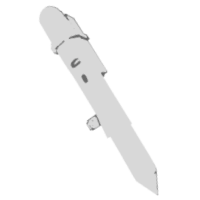
\includegraphics[width=0.25\textwidth]{imagenes/LogoSmartPen.png} 
 \vspace{0.5cm}

% Title

{\Huge\bfseries Dispositivo para detección de escritura mediante Deep Learning en
un sistema empotrado\\
}
\noindent\rule[-1ex]{\textwidth}{3pt}\\[3.5ex]
{\large\bfseries SmartPen\\[4cm]}
\end{minipage}

\vspace{2.5cm}
\noindent\hspace*{\centeroffset}\begin{minipage}{\textwidth}
\centering

\textbf{Autor}\\ {Antonio Priego Raya}\\[2.5ex]
\textbf{Directores}\\
{Juan José Escobar Pérez\\
Jesús González Peñalver}\\[2cm]
%
\includegraphics[width=0.15\textwidth]{imagenes/tstc.png}\\[0.1cm]
%\textsc{Departamento de Teoría de la Señal, Telemática y Comunicaciones}\\
%\textsc{---}\\
%Granada, mes de 201
\end{minipage}
%\addtolength{\textwidth}{\centeroffset}
\vspace{\stretch{2}}

 
\end{titlepage}






\cleardoublepage
\thispagestyle{empty}

\begin{center}
{\large\bfseries Detección de escritura mediante Deep Learning en
un sistema empotrado\\
}
\textsc{---}\\
{\small\bfseries Deep Learning en sistemas empotrados: TinyML.}\\
\end{center}
\begin{center}
Antonio Priego Raya\\
\end{center}

%\vspace{0.7cm}
\noindent{\textbf{Palabras clave}: TinyML, Machine learning, Deep learning,
Sistemas empotrados, Reconocimiento letras, Redes neuronales convolucionales,
...}\\

\vspace{0.7cm}
\noindent{\textbf{Resumen}}\\

\begin{comment}
Creación de un dispositivo autónomo con forma de lápiz en el que integrar un
sistema empotrado, concretamente haré uso de la Arduino Nano Sense 33 BLE.
El propósito de este dispositivo será la detección de letras en tiempo
real, registrando el movimiento del dispositivo para resolver la detección
de estas.\\
Para el procesamiento y clasificación de los movimientos se empleará
deep learning, con un modelo de red neuronal convolucional. Con la
particularidad de ejecutar el procesamiento del modelo en el propio
dispositivo, para dotarlo de autonomía.\\
Por tanto se desarrollarán todos los pasos propios del trabajo con
redes neuronales: diseño del modelo, recolección de datos, entrenamiento
del modelo, etc.\\
Complementario al dispositivo, también se creará un interfaz donde acceder
a las funciones del dispositivo.
\end{comment}
\cleardoublepage


\thispagestyle{empty}


\begin{center}
{\large\bfseries Project Title: Project Subtitle}\\
\end{center}
\begin{center}
First name, Family name (student)\\
\end{center}

%\vspace{0.7cm}
\noindent{\textbf{Keywords}: Keyword1, Keyword2, Keyword3, ....}\\

\vspace{0.7cm}
\noindent{\textbf{Abstract}}\\

Write here the abstract in English.

\chapter*{}
\thispagestyle{empty}

\noindent\rule[-1ex]{\textwidth}{2pt}\\[4.5ex]

Yo, \textbf{Antonio Priego Raya}, alumno de la titulación \textit{Grado en Ingeniería Informática}
de la \textbf{Escuela Técnica Superior
de Ingenierías Informática y de Telecomunicación de la Universidad de Granada}, con DNI 31033948W, autorizo la
ubicación de la siguiente copia de mi Trabajo Fin de Grado en la biblioteca del centro para que pueda ser
consultada por las personas que lo deseen.

\vspace{6cm}

\noindent Fdo: Antonio Priego Raya

\vspace{2cm}

\begin{flushright}
Granada a DÍA de Junio de 2022
\end{flushright}


\chapter*{}
\thispagestyle{empty}

\noindent\rule[-1ex]{\textwidth}{2pt}\\[4.5ex]

D. \textbf{Jesús González Peñalver}, Catedrático del departamento de Arquitectura y Tecnología de Computadores de la Universidad de Granada.

\vspace{0.5cm}

D. \textbf{Juan José Escobar Pérez}, Profesor Sustituto Interino del departamento de Arquitectura y Tecnología de Computadores de la Universidad de Granada.

\vspace{0.5cm}

\textbf{Informan:}

\vspace{0.5cm}

Que el presente trabajo, titulado \textit{\textbf{Dispositivo para detección de escritura mediante Deep Learning en
un sistema empotrado}},
ha sido realizado bajo su supervisión por \textbf{Antonio Priego Raya}, y autorizamos la defensa de dicho trabajo ante el tribunal
que corresponda.

\vspace{0.5cm}

Y para que conste, expiden y firman el presente informe en Granada a X de mes Julio de 2022.

\vspace{1cm}

\textbf{Los directores:}

\vspace{5cm}

\noindent \textbf{Jesús González Peñalver \ \ \ \ \ \ \ \ \ \ \ Juan José Escobar Pérez}

\chapter*{Agradecimientos}
\thispagestyle{empty}

       \vspace{1cm}


Poner aquí agradecimientos...



	
	% Índice de contenidos
	\newpage
	\tableofcontents

	% Índice de imágenes y tablas
	\newpage
	\listoffigures

	% Introducción 
	\chapter{Introducción y Motivación}
Como consecuencia del desarrollo de la informática, y la expansión y
filtración del uso de equipos informáticos en la población general,
cada vez la escritura tradicional cae más en desuso. Y es que una
vez se supera la etapa académica, pocas personas siguen utilizando
en su cotidianidad la escritura manual. Incluso para la educación
hay un creciente movimiento de adaptación tecnológica que releva
cada vez más al lápiz y papel.\newline
No es el objetivo pecar de romanticismo y mirar a través de la lente
de la nostalgia, sino avanzar, eso sí, intentando conservar en el proceso
de innovación, las técnicas que nos han traído hasta aquí.

Por lo que el motivo de este trabajo siempre ha sido tratar de,
creando nueva tecnología, favorecer el uso de la escritura.
Ya que el avance y el progreso es no solo imparable sino necesario,
la única forma de preservación de la grafía manual es establecer
alternativas modernas que complementen a los dispositivos ya
constituidos y que empleamos en el día a día.

Gracias al avance tecnológico de décadas, hoy podemos contar con
herramientas informáticas de gran capacidad como lo son todos
los mecanismos de Inteligencia Artificial. Concretamente el Deep
Learning y las redes neuronales son conceptos en gran expansión
durante los últimos años.
{\color{migris} El \textit{Deep Learning} es un campo que está cambiando
la informática como la concebíamos, revelándose como una alternativa
sobresaliente para problemas que trabajan con grandes volúmenes de
información, que presentan una elevada complejidad o simplemente
que cumplen mejor de lo que habituaban a hacerlo con técnicas
previas. Respondiendo oportunamente al contexto temporal vigente
donde el \textit{Big Data}, \textit{Data Science}, automatización
de tareas cotidianas, detonación de herramientas y dispositivos
inteligentes, humanización de robots y robotización de personas;
perfilan y caracterizan la fase en la que nos encontramos.
Hecho que nos lleva al interés por un terreno tan intrincado
como útil y repleto de potencial. Un potencial evidenciado por
las tantas aplicaciones con sobrecogedores resultados que hace pocos
años casaban más con la ciencia ficción que con algo alcanzable, y que
emplean esta herramienta y que serán citadas a lo largo de este trabajo.
}

Por sus demostradas altas capacidades para
la clasificación en el procesamiento de imagen, por el hito
que supuso integrar redes neuronales en sistemas tan reducidos,
porque hay algo sugestivo en el hecho de rescatar lo tradicional
mediante las técnicas más incipientes,
pero por encima de todo, por lo estimulante que resulta trabajar con
estos mecanismos y que es algo que siempre ha rondado entre mis pensamientos;
este trabajo consistirá
en trasladar a la realidad una alternativa moderna a la escritura
manual, haciendo uso de Deep Learning en un sistema empotrado
para mantener autonomía.

{\color{migris}Los usos pueden ser los que se deseen y se alcancen a imaginar;
con pocos añadidos podría convertirse en una herramienta para
introducir a personas de avanzada edad al manejo de ordenadores, reduciendo
la barrera de entrada al tener una forma de interactuar que ya les es familiar;
en un instrumento para hacer más ameno y dinámico el proceso de aprender
a escribir para niños y niñas; en un cuaderno virtual en el que anotar cuanto queramos sin necesidad de
transportar el medio en el que se escribe; incorporando una punta
con grafito o tinta, podríamos transcribir digitalmente lo que escribimos
en cada momento de manera física, es decir, una copia digital, un registro
de lo que hemos escrito; etc.}

\begin{comment}
Pero por qué no unir ambas experiencias para obtener la sensación de
escritura tradicional y la pretensión pragmática de utilizar nuevas
tecnologías.\\

Es lo que se plantea en este proyecto, un dispositivo que, haciendo
uso de las técnicas más modernas de inteligencia artificial, ayude a
la preservación de la escritura manual; facilitando la inclusión de
la misma en el uso ordinario de los dispositivos electrónicos.\\

Asimismo, en algunos casos sería una forma de incentivar e introducir
a personas poco habituadas al uso de la tecnología, ya que el hecho
de enfrentarse a un nuevo instrumento, puede suponer una barrera
psicológica al empezar para personas de avanzada edad.\newline
Otra posibilidad es enfocarlo como herramienta didáctica, para
que los niños aprendan a escribir de una forma divertida y atractiva.\\ 

Por tanto, el objetivo de este proyecto es desarrollar no solo
un dispositivo autónomo de captación de escritura manual, sino
un entorno completo con la finalidad de diluir la barrera entre
lo tradicional y lo moderno.
\end{comment}

	% Descripción del problema y hasta donde se llega
	%\chapter{Descripción del problema}



	% Análisis del problema
	% 1. Análisis de requisitos
	% 2. Análisis de las soluciones
	% 3. Solucion propuesta
	% 4. Análisis de seguridad
	%\chapter{Análisis del problema}
 


	% Estado del arte
	\chapter{Antecedentes y estado actual}
\section{Redes neuronales}
Pese a que es ahora, en los últimos años cuando, debido a la explosión
del fenomeno de la \textit{inteligencia artificial}, comienza a ser
más popular todo lo relacionado con la dotación de inteligencia a
los dispositivos electrónicos; todo comenzó hace muchas décadas\textsuperscript{\cite{na8}}.
Ya en 1943, \textit{Warren McCulloch} (neurofisiologo) y
\textit{Walter Pitts} (matemático),
escribieron un artículo\textsuperscript{\cite{McCulloch}} acerca de las neuronas e incluso en el mismo,
fueron capaces de diseñar una red neuronal simple usando exclusivamente
circuitos eléctricos y fundamentado en algoritmos de \textit{Lógica de umbral}
(\textit{Threshold logic}).


Más tarde, en la década de 1950, en los laboratorios de \textit{IBM} de
la mano de \textit{Nathanial Rochester}, ocurrió el primer
intento de simulación de red neuronal; intento que desembocó en fracaso.
Sin embargo fue muy estimulante para el campo de la \textit{IA}
y motivó el planteamiento de lo que denominaron "máquinas pensantes".
También hubo otros acercamientos como la sugerencia del insigne
\textit{John Von Neumann} de utilizar relés telegráficos o
tubos de vacío para simular el funcionamiento simplificado de
las neuronas.


No obstante, no sería hasta 1958 que el neurobiólogo
\textit{Frank Rosenblatt} comenzaría a trabajar en el \textit{Perceptron}\textsuperscript{\cite{Rosenblatt}},
para muchos el nacimiento de la red neuronal artificial. Como todo precursor,
era simple y limitado; hoy se catalogaría de monocapa, algo que evidentemente,
ya no se usa en redes neuronales contemporaneas.
Como puede observarse en la Figura \ref{perceptron} sirviéndose de múltiples entradas binarias, era capaz de producir una
única salida, basada ya entonces en la utilización de \textit{pesos}
(número que cuantifica la relevacia de la entrada respecto de la salida),
conservada hasta día de hoy, aunque cabe destacar que entonces, los pesos
eran directamente atribuidos por el científico al cargo.
La salida binaria de esta neurona \textit{Perceptron},
sería como consecuencia de la superioridad o la inferioridad de la
suma de la multiplicación de los pesos respecto de un umbral; es por esto
que es sabida su influencia del trabajo de \textit{Warren McCulloch} y
\textit{Walter Pitts} anteriormente mencionado. Por tanto se podía destinar
a funciones lógicas binarias simples (OR/AND).


El siguiente paso natural era aumentar el número neuronas y capas,
llegando en 1965 el \textit{Multilayer Perceptron}
\textit{Perceptron}\textsuperscript{\cite{mlperceptron}}. Como consecuencia
de esta mejora y aumento de la complejidad, nacieron los conceptos de
capas de entrada, ocultas y de salida, tal y como se puede observar en la
Figura \ref{MLPerceptron}. De igual forma y dado que el
reparto de pesos todavía no se había automatizado, los valores con los
que se trabajaban, seguían siendo binarios.

\begin{figure}[h]
    \centering
    \subfloat[Perceptron\label{perceptron}]{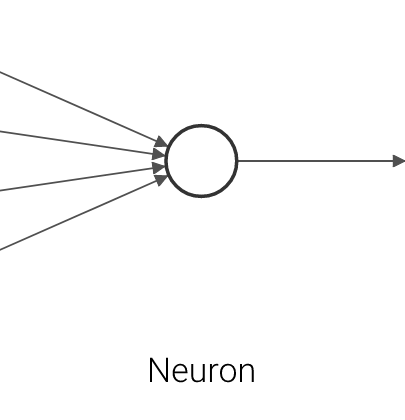
\includegraphics[width=0.25\textwidth]{capturas/esquemaPerceptron.png}}
    \hfill
    \subfloat[Multilayer Perceptron\label{MLPerceptron}]{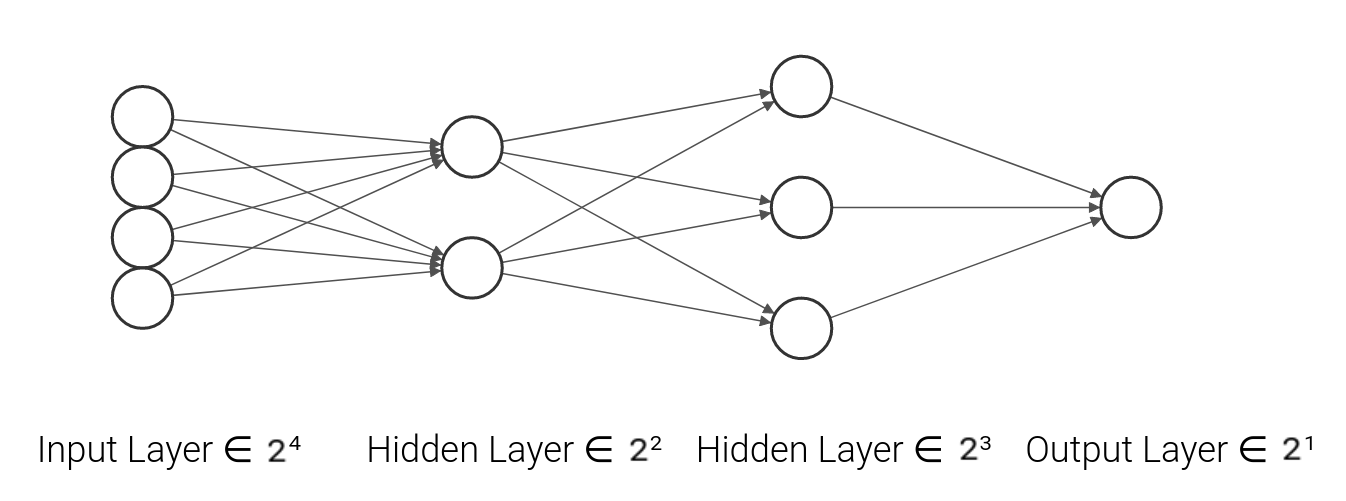
\includegraphics[width=0.75\textwidth]{capturas/esquemaMLPerceptron.png}}
    \caption{\textit{Perceptron} frente a \textit{Multilayer Perceptron}}
  \end{figure}


Y este fue precisamente el siguiente escalón a rebasar, superado ya en
la década de 1980, gracias a las \textit{Neuronas Sigmoides}
\textit{Perceptron}\textsuperscript{\cite{sancho}}, afines al
\textit{Perceptron} pero con la capacidad de trabajar con números reales.
La función de salida ahora sería una sigmoide, a la que deben su nombre y
convirtiéndose en la primera función de activación.

A partir de aquí y durante toda la década, comenzaron a aparecer todo tipo
de novedades que continúan vigentes: redes \textit{feedforward}, el algoritmo
\textit{backpropagation} o la \textit{Red Neuronal Convolucional}
(\textit{Convolutional Neural Network}, CNN)\textsuperscript{\cite{geo}}.
Las \textit{CNN} son especialmente convenientes para procesamiento de
imagen y vídeo, en general información espacial, aunque también se han
usado para tareas de procesamiento
de lenguaje natural. Esto es debido a que la información se divide en subcampos que sirven como
entrada a capas de procesamiento convolucional (ver Figura \ref{cnn}), encargadas de apreciar
las distintas carcterísticas que servirán para la clasificación de la
información de entrada.

\begin{figure}[h]
    \centering
    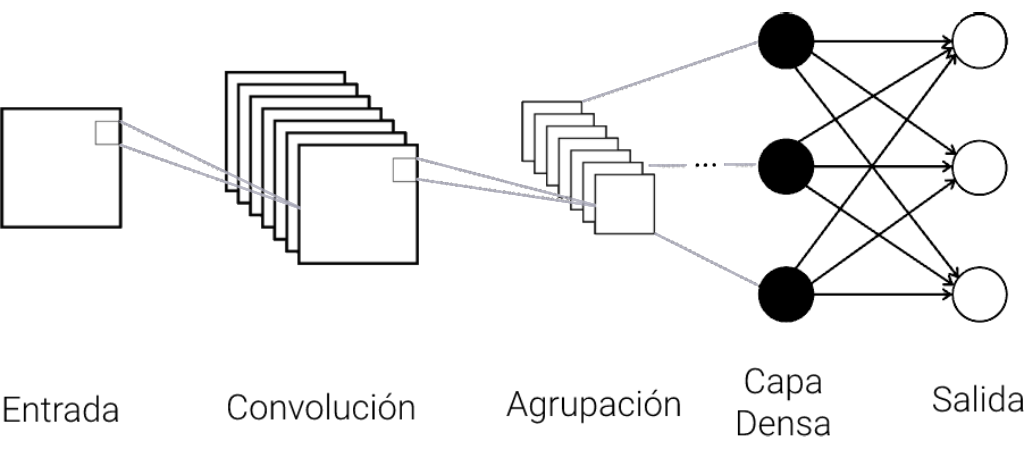
\includegraphics[width=0.69\textwidth]{capturas/CNN.png}\\[-0,20cm]
    \caption{Estructura simplificada de \textit{Red Neuronal Convolucional}\label{cnn}}
\end{figure}

Es llamativo ver cómo las \textit{CNN}, redes que mantienen su vigencia
pese a que su origen se remonta a poco antes de los 90. Pero la realidad es
que, si bien no lo parece, el campo de las redes neuronales lleva con nosotros
mucho tiempo y las \textit{CNN} no son el único ejemplo manifiesto.
Las \textit{Recurrent Neural Networks}, originadas en 1989, continúan en
uso para procesamiento de datos secuenciales como lo es por ejemplo el texto.

Fue en 2006 cuando \textit{Geoffrey Hinton et al} publicaron un famoso
paper\textsuperscript{\cite{hinton}} presentando una red neuronal profunda,
que entrenada, era capaz de reconocer dígitos. Acuñando como \textit{Deep Learning},
a la técnica del \textit{Machine Learning} (ya que se basa en el aprendizaje
automático), que usa como mecanismo de procesamiento redes neuronales profundas.
Se superaba entonces la barrera del entrenamiento de redes neuronales profundas,
barrera que había llevado a la comunidad a congelar el avance de esta técnica,
y que ahora elevaba al \textit{Deep Learning}
un nivel por encima del resto de técnicas del \textit{Machine Learning}.

El siguiente hito llegaría a mediados de los 2000 al poder trabajar
con redes neuronales profundas (\textit{Deep Learning}), gracias a la
introducción de pre-entrenamientos no supervisados para la asignación
de pesos previos al usual entrenamiento del modelo. Este avance fue
posible debido al desarrollo de la computación con GPUs.


El último acontecimiento o adición reseñable es el de las
\textit{Generative Adversarial Networks} (2014)
\textsuperscript{\cite{genAd}}, sujeto al empleo de dos
redes neuronales complementarias: una se denomina \textit{Generative network}
en calidad de modelo generador de muestras y otra \textit{Discriminative network}
que evalúa las muestras generadas por la anterior y por el dataset de entrenamiento,
es decir, recibe como entrada, la salida de la red anterior y del conjunto
de datos de entrenamiento. El proposito de esta simbiosis es que la red
generativa consiga reproducir muestras tan válidas como las de entrenamiento,
a partir del juicio de la red discriminativa.


De entonces hasta ahora, más que innovación, se han dado muchos avances
en términos de implementación, es habitual que cada cierto tiempo salga
una nueva aplicación revolucionaria o con mucho potencial que está basada
en redes neuronales. Y también es muy frecuente que gigantes tecnológicos
como por ejemplo \textit{Google} o \textit{Facebook} compren otros
proyectos basados en redes neuronales o directamente las empresas
que los llevan a cabo. Siendo una de las más destacables la compra de
\textit{DeepMind} por parte de \textit{Google} o la alianza entre
\textit{OpenIA} y \textit{Microsoft}.


Algunos ejemplos de estos proyectos son:
el tan sonado algoritmo de \textit{AlphaGo}\textsuperscript{\cite{alphago}}
de la empresa \textit{DeepMind},
capaz de vencer al campeón mundial del juego tablero \textit{Go}; el
proyecto \textit{DeepFace} de \textit{Facebook} para identificar y automatizar
el etiquetado de los usuarios en las imágenes; el \textit{AlphaFold2}
\textsuperscript{\cite{alphafold}} de
\textit{DeepMind}, capaz de predecir la estructura de las proteínas y que
ha sido revolucionario para la resolución del problema del plegamiento de
proteínas, lo que antes eran investigaciones del orden de 1 o 2 años, ahora
es computable en pocas horas; \textit{GPT-3}
\textsuperscript{\cite{openai}} de \textit{OpenIA},
un modelo de lenguaje cuya definición podría responder a \textit{chatbot},
es capaz de completar texto, responder preguntas o cualquier tarea que
implique interacción con texto; \textit{Copilot}\textsuperscript{\cite{ghcopilot}}
de \textit{OpenIA}
y \textit{Github, Microsoft}, un sistema construido sobre los cimientos de
\textit{GPT-3} capaz de sugerir código autogenerado
y comentarios analizando bien las directrices de un comentario o bien
directamente interpretando lo que el programador busca; \textit{Nerf}\textsuperscript{\cite{nerfs}}
de \textit{Nvidia}, capaz de generar composiciones 3D a partir de
imágenes fíjas; o por finalizar esta interminable lista de apasionantes
ejemplos, el reciente \textit{DALL.E}\textsuperscript{\cite{openai}} de \textit{OpenAI}, modelo generador
de imágenes a partir de una entrada de texto descriptora.

No se puede quedar sin mencionar las que han sido las dos últimas grandes
agitaciones del mundo de las redes neuronales y que están detrás de la
mayoría de los ejemplos anteriores: el \textit{Natural Language Processing}
y los \textit{Transformers}, aunque en realidad, van de la mano.
Van de la mano porque el \textit{Natural Language Processing}\textsuperscript{\cite{nlp}}
ya es
en sí mismo una revolución para el mundo de las redes neuronales, ya que
el procesamiento de lenguaje, dado que las redes interpretan información
numérica, siempre ha sido un desafío para el campo del \textit{Machine Learning};
y no ha sido hasta su llegada, que gracias a lo que propone (vectorización de
\textit{tokens}, que son los bloques de datos que se interpretan, ya sean
palabras o generalmente en la práctica, subpalabras), que las redes
no han empezado a operar de una forma realmente veraz con el lenguaje.
Sin embargo no solo ha sido una revolución en sí mismo, sino que ha
propiciado el nacimiento de otra como lo son los \textit{Transformers}\textsuperscript{\cite{transformers}},
que parten del progreso conseguido en las redes recurrentes o para ser más
precisos, de sus \textit{Mecanismos de Atención}\textsuperscript{\cite{aiayn}},
ya que es lo único que
mantienen respecto a los modelos recurrentes, es más, se alejan íntegramente
pasando a un procesamiento simultáneo y sustituyendo la ordenación recurrente
por la vectorización. Aunque pese a renunciar a la recurrencia, y es ahí donde
reside su potencial, continúan funcionando con información secuencial.

Esta mejora en la implementación y aparición de tantas aplicaciones
puede inferirse que se debe al aumento de la capacidad de cómputo de
las GPUs, la llegada de los \textit{Transformers},
la entrada de los mayores gigantes tecnológicos, pero sin
duda a la aparición de herramientas de alto nivel e infraestructuras
para el trabajo con redes neuronales como lo son \textit{Azure},
\textit{Aporia}, \textit{TensorFlow}, \textit{Keras}, \textit{SciKit-Learn},
etc.

\section{Microcontroladores}
Los microcontroladores son sistemas de dimensiones reducidas y bajo consumo,
destinados en su inicio al control de electrodomésticos, pero que a lo largo
del tiempo y sobre todo propiciado por la aparición del
\textit{Internet of things} (\textit{IoT}), y los avances en \textit{IA} han
supuesto un cambio en cómo se diseñan e implementan los nuevos dispositivos
electrónicos.

El primer microcontrolador fue desarrollado por \textit{Gary Boone} y
\textit{Michael Cochran} en 1971 y fue bautizado como
\textit{TSM 1000}\textsuperscript{\cite{mccon}}, albergando una arquitectura
\textit{Harvard} en un mismo circuito contando con el propio microprocesador,
memoria ROM, menos de 256 bytes de memoria RAM y el propio reloj del sistema.

Como respuesta, \textit{Intel} comercializó en 1977 su propio sistema para
aplicaciones de control, el \textit{Intel 8048}\textsuperscript{\cite{mcs48}},
que obtuvo gran popularidad y supuso un pequeño cambio en el paradigma de
ventas de \textit{Intel}.

Las memorias que montaban eran \textit{EPROM} en el caso de los microcontroladores
reprogramables y \textit{PROM} en el caso de los de bajo  presupuesto. Sin embargo esto
cambió con la llegada en 1993 de la \textit{EEPROM}, utilizada por primera vez
en el \textit{PIC16x64}\textsuperscript{\cite{mccon}} de \textit{Microchip} y que conllevó un gran avance
gracias a la agilización del proceso de creación de prototipos y su programación.

Poco después \textit{Atmel} implementaría por primera vez memoria \textit{flash}
en un microcontrolador y se usaría en el \textit{Intel 8051}, que trajo
ciertos cambios respecto a su predecesor, como pasar a arquitectura
\textit{Von Neumann} o la inclusión de
\textit{Universal Asynchronous Receiver-Transmitter}
(\textit{UART}) para el manejo de puertos y dispositivos serie. Además contaba
con múltiples compiladores de \textit{C} para su programación, alternativos
al lenguaje \textit{ensamblador}.

Gracias a la inclusión de estas dos últimas memorias en el diseño estandarizado de
los microcontroladores, el precio comenzó a ser cada vez más accesible.
También se inició la incorporación de periféricos complementarios para dotar
a los microcontroladores de más funcionalidad. Periféricos tales como generadores
\textit{PWM}, conversores analógicos A/D y D/A, relojes de tiempo real, etc.

Estos complementos lucen ahora arcaicos en comparación con los que se integran
en microcontroladores actuales: transceptores 802.15.4, bluetooh, wifi, cámaras,
micrófonos, y sensores de todo tipo como de presión, movimiento, orientación, color,
brillo, proximidad, humedad, etc. Todos estos acompañados de complejos microprocesadores
de 32 bits, cada vez más semejantes a las \textit{CPU}s de equipos de mayores
dimensiones. El progreso de los microprocesadores reducidos, ha sido propiciado
por el vasto crecimiento del mercado móvil en los últimos años. Y resultando
\textit{ARM}, al igual que para los smartphones, una excelente baza para la
complejidad que demandan los microcontroladores actuales.

Por un lado, su contenida complejidad frente a equipos de escritorio, hace que
económicamente su implementación sea muy viable, aunque esto mismo provoca
ciertos inconvenientes a la hora de su empleabilidad para \textit{IA}, mencionados
en la siguiente sección.


\section{Integración de redes neuronales en microcontroladores\label{integRNenμC}}
Algunos microcontroladores modernos dan soporte a herramientas para la \textit{IA},
como lo es la integración de redes neuronales;
sin embargo, el desarrollo de estas sigue siendo dependiente de la asistencia de un
PC. De igual forma este soporte a herramientas para la \textit{IA} es aun así
sorprendente viendo los resultados que se pueden obtener de su implementación y
siendo este proyecto muestra de ello.
Aunque en algunas ocasiones son necesarios ciertos arreglos dadas las carencias
de estos dispositivos, como en ciertos casos, la falta de \textit{FPU}s
(\textit{Floating-Point Unit}), suponiendo un obstáculo debido a que las redes
neuronales realizan su procesamiento en coma flotante.

Se precisa de equipos con mayores prestaciones para la
creación y entrenamiento de las redes neuronales que integrarán los microcontroladores,
ya que es un proceso complejo y costoso;
por suerte no es así para la ejecución, lo que los convierte en grandes candidatos
gracias al \textit{CloudML}, \textit{EdgeML} o \textit{TinyML}.

El \textit{CloudML}\textsuperscript{\cite{CloudMl}} es la técnica por la que, alojando redes neuronales profundas
en la nube, podemos integrar el uso de las mismas en \textit{TPU}s (Unidades de procesamiento
tensorial) y \textit{FPGA}s, entre otras. Esta alternativa presenta la capacidad
de emancipar el propio procesamiento de los algoritmos de \textit{Macine Learning}
fuera del propio dispositivo en el que se integra su implementación. Por otro lado,
supone contar con infraestructuras que den soporte a ello y el uso de herramientas
y entornos de pago, como entre otros el \textit{Google Cloud ML Engine}.

\textit{EdgeML}\textsuperscript{\cite{EdgeMl}} es una librería escrita en \textit{Python} propulsada por
\textit{GitHub, Microsoft} que mediante \textit{TensorFlow} (o alternativamente en
fase experimental \textit{Pytorch}), provee de distintas funciones enfocadas al
entrenamiento, evaluación y despliegue de algoritmos de
\textit{Machine Learning} para sistemas embebidos empleados para labores simples.
Por lo que es una elección perfecta para aquellos proyectos en los que se quiera
trabajar con \textit{Machine Learning} y utilizar herramientas de apoyo
\textit{open source}. Aunque cabe mencionar que, al tratarse de una herramienta
para \textit{Machine Learning} en general, las opciones dirigidas a
\textit{Deep Learning} no abundan.

\textit{Micro-Learn}\textsuperscript{\cite{microlearn}} es una librería para
\textit{python} que convierte modelos de \textit{machine learning} entrenados
con \textit{Scikit-Learn},
a código que virtualiza la ejecución del modelo en cualquier microcontrolador
en tiempo real.
Es relevante destacar que no existen demasiados proyectos, aunque a cambio
ofrece, en principio, soporte para cualquier microcontrolador \textit{arduino}.

También existen infinidad de destacables alternativas para \textit{FPGA}s como
\textit{Vitis-AI} o \textit{VTA}, entre otras, aunque no presentan soporte a
microcontroladores, por lo que quedan fuera de nuestro espectro de posibilidades.

Y finalmente, \textit{TinyML}\textsuperscript{\cite{tinyMl}} se define como el
campo que comprende a las tecnologías y aplicaciones relacionadas con el
\textit{Machine Learning} y que se fundamenta en la implementación de algoritmos
y software capaces de realizar análisis de datos de sensores en un hardware
muy limitado y de bajo consumo energético. Encontrando en esta alternativa,
numerosos proyectos que consultar, gran actividad de su comunidad y cuantiosa
documentación en forma de libros y publicaciones de usuarios.

\begin{comment}
En el campo del \textit{Deep Learning} integrado en sistemas empotrados, hay múltiples proyectos que
poder estudiar y observar previos a comenzar nuestro trabajo.\\\\
Disponemos, en el caso preciso de Arduino, aunque como sabemos no es el único fabricante de
este tipo de dispositivos; de una plataforma donde se exponen numerosos ejemplos de entusiastas
de Arduino que publican de forma abierta su código\cite{project-hub}. Y entre todos ellos, podemos encontrar
varios planteamientos haciendo uso de \textit{Machine Learning} como herramienta de procesamiento procesamiento.
\newline Estos proyectos suelen haberse diseñado para la placa con la que trabajaremos, ya que es no
hay plétora de dispositivos que posean capacidad de trabajar con TensorFlow.\\
La mayoría de los proyectos que podemos encontrar, son más demostraciones técnias y pequeñas
introducciones al trabajo con \textit{TensorFlow}, que proyectos con alguna finalidad. Pero aun así, me
han sido de enorme utilidad para entablar contacto con el entorno y dinámica de trabajo.\\
Hay uno de estos trabajos, o más que trabajos, desarrolladores, que ha sido un pilar para este
proyecto; se trata de \textit{Pete Warden}, probablemente la persona más ilustre en \textit{TensorFlow+Arduino}.
\textit{Pete Warden} es entre otros, el creador de uno de los libros que ha sido determinante para
documentarme y comenzar con TinyML: "\textit{TinyML: Machine Learning with TensorFlow Lite on
Arduino and Ultra-Low-Power Microcontrollers}"\cite{TinyML-PW}.\\
El \textit{magic\_wand}\cite{github-magicwand} de Arduino fue para mí la toma de contacto precedente a comenzar a realizar mi propio
código. Sin embargo fue la versión de \textit{Pete Warden}\cite{petewardenmw} la que ha servido como cimiento al desarrollo
del software que cargaré en la placa y en el que he terminado de comprender las dinámicas de trabajo
para TinyML.\\

Respecto al diseño y entrenamiento del modelo, no hay demasiados referentes.
Pero cabe destacar lo muy conveniente que es el libro "\textit{Hands-on Machine Learning
with Scikit-Learn, Keras, and TensorFlow}"\cite{Aurelien}. No solo estimable para TinyML, sino
para comprender muchos de los conceptos generales y bases teóricas y matemáticas
de \textit{TensorFlow}. Incluso como introducción a la práctica para crear tus primeros modelos,
ya que como se infiere del título, también se tratan herramientas de alto nivel que facilitan
la implementación de los modelos como lo son \textit{Scikit} o \textit{Keras}. Esta última
será esencial para nuestro planteamiento de modelo.
\end{comment}

	% Análisis de requisitos
	\input{capitulos/03_Especificación_del_sistema.tex}

	% Diseño del sistema completo
	\input{capitulos/04_Diseño_del_sistema.tex}

	% Skectch cargado en la placa
	\chapter{Microcontrolador}
\section{Planificación}
En la planificación se recogerá la elección de equipo y herramientas de desarrollo
previas al diseño.
\subsection{Elección del microcontrolador}
Como ya se especificó en la sección \textit{(\ref{reqHW})Requisitos hardware}
necesitamos ciertas características inmutables. Para poder quedarnos con un
microcontrolador, antes debemos hacer el ejercicio de búsqueda de algunos
candidatos y analizar sus características. La búsqueda se ha sustentado
en encontrar dispositivos compatibles con \textit{TensorFlow Lite}.
\begin{table}[h]
    \color{mitexto}
    \begin{tabular}{|l|c|c|c|ccc|}
        \hline
        \rowcolor[HTML]{6C737E} 
        \multicolumn{1}{|c|}{\cellcolor[HTML]{6C737E}{\color[HTML]{EFEFEF} \rotatebox{284}{\textbf{Microcontrolador~}}}} & \cellcolor[HTML]{6C737E}{\color[HTML]{EFEFEF} \rotatebox{284}{\textbf{Precio~}}} & {\color[HTML]{EFEFEF} \rotatebox{284}{\textbf{Documentación~}}} & {\color[HTML]{EFEFEF} \rotatebox{284}{\textbf{Dimensiones~}}} & {\color[HTML]{EFEFEF} \rotatebox{284}{\textbf{Sensores~}}}       & {\color[HTML]{EFEFEF} \rotatebox{284}{\textbf{Disponibilidad~}}} & {\color[HTML]{EFEFEF} \rotatebox{284}{\textbf{Soporte para DL~}}} \\ \hline
        {\cellcolor[HTML]{CDDADE}SparkFun Edge}                                                        & {\cellcolor[HTML]{CDDADE}{\color[HTML]{4CDE4C} \cmark}}            & {\cellcolor[HTML]{CDDADE}{\color[HTML]{4CDE4C} \cmark}}                 & {\cellcolor[HTML]{CDDADE}{\color[HTML]{9B9B9B} -}}                        & \multicolumn{1}{c|}{{\cellcolor[HTML]{CDDADE}{\color[HTML]{4CDE4C} \cmark}}} & \multicolumn{1}{c|}{{\cellcolor[HTML]{CDDADE}{\color[HTML]{9B9B9B} -}}}      & {\cellcolor[HTML]{CDDADE}{\color[HTML]{4CDE4C} \cmark}}                       \\
        {\cellcolor[HTML]{E8ECF1}Arduino Nano Sense 33 BLE}                                            & {\cellcolor[HTML]{E8ECF1}{\color[HTML]{4CDE4C} \cmark}}            & {\cellcolor[HTML]{E8ECF1}{\color[HTML]{4CDE4C} \cmark}}                 & {\cellcolor[HTML]{E8ECF1}{\color[HTML]{4CDE4C} \cmark}}                   & \multicolumn{1}{c|}{{\cellcolor[HTML]{E8ECF1}{\color[HTML]{4CDE4C} \cmark}}} & \multicolumn{1}{c|}{{\cellcolor[HTML]{E8ECF1}{\color[HTML]{9B9B9B} -}}}      & {\cellcolor[HTML]{E8ECF1}{\color[HTML]{4CDE4C} \cmark}}                       \\
        {\cellcolor[HTML]{CDDADE}STM32F746G}                                                           & {\cellcolor[HTML]{CDDADE}{\color[HTML]{FD6864} \xmark}}            & {\cellcolor[HTML]{CDDADE}{\color[HTML]{9B9B9B} -}}                      & {\cellcolor[HTML]{CDDADE}{\color[HTML]{FD6864} \xmark}}                   & \multicolumn{1}{c|}{{\cellcolor[HTML]{CDDADE}{\color[HTML]{4CDE4C} \cmark}}} & \multicolumn{1}{c|}{{\cellcolor[HTML]{CDDADE}{\color[HTML]{4CDE4C} \cmark}}} & {\cellcolor[HTML]{CDDADE}{\color[HTML]{4CDE4C} \cmark}}                       \\
        {\cellcolor[HTML]{E8ECF1}Adafruit EdgeBadge}                                                   & {\cellcolor[HTML]{E8ECF1}{\color[HTML]{4CDE4C} \cmark}}            & {\cellcolor[HTML]{E8ECF1}{\color[HTML]{4CDE4C} \cmark}}                 & {\cellcolor[HTML]{E8ECF1}{\color[HTML]{FD6864} \xmark}}                   & \multicolumn{1}{c|}{{\cellcolor[HTML]{E8ECF1}{\color[HTML]{4CDE4C} \cmark}}} & \multicolumn{1}{c|}{{\cellcolor[HTML]{E8ECF1}{\color[HTML]{9B9B9B} -}}}      & {\cellcolor[HTML]{E8ECF1}{\color[HTML]{4CDE4C} \cmark}}                       \\
        {\cellcolor[HTML]{CDDADE}STM32}                                                                & {\cellcolor[HTML]{CDDADE}{\color[HTML]{4CDE4C} \cmark}}            & {\cellcolor[HTML]{CDDADE}{\color[HTML]{9B9B9B} -}}                      & {\cellcolor[HTML]{CDDADE}{\color[HTML]{4CDE4C} \cmark}}                   & \multicolumn{1}{c|}{{\cellcolor[HTML]{CDDADE}{\color[HTML]{FD6864} \xmark}}} & \multicolumn{1}{c|}{{\cellcolor[HTML]{CDDADE}{\color[HTML]{4CDE4C} \cmark}}} & {\cellcolor[HTML]{CDDADE}{\color[HTML]{4CDE4C} \cmark}}                       \\
        {\cellcolor[HTML]{E8ECF1}ESP32}                                                                & {\cellcolor[HTML]{E8ECF1}{\color[HTML]{4CDE4C} \cmark}}            & {\cellcolor[HTML]{E8ECF1}{\color[HTML]{9B9B9B} -}}                      & {\cellcolor[HTML]{E8ECF1}{\color[HTML]{4CDE4C} \cmark}}                   & \multicolumn{1}{c|}{{\cellcolor[HTML]{E8ECF1}{\color[HTML]{FD6864} \xmark}}} & \multicolumn{1}{c|}{{\cellcolor[HTML]{E8ECF1}{\color[HTML]{4CDE4C} \cmark}}} & {\cellcolor[HTML]{E8ECF1}{\color[HTML]{4CDE4C} \cmark}}                       \\ \hline
    \end{tabular}
    \caption{Tabla de requisitos para elección de microcontrolador}
\end{table}

La \textit{ESP32} al igual que la \textit{STM32} pueden descartarse debido a que
carecen de sensores relacionados
con el movimiento, se les podrían integrar periféricamente, pero sería algo
más molesta su inserción en una carcasa. Y dado que tenemos alternativas que
cuentan con estos sensores, podemos permitirnos descartarlas.

Por otro lado la \textit{Adafruit EdgeBadge} es una placa muy llamativa,
potente y llena de posibilidades, pero cuenta con unas dimensiones superiores
a lo que se busca.

Respecto a la \textit{STM32F746G} el inconveniente es la bajísima disponibilidad
y los plazos de envío desorbitados. Por tanto tampoco podemos contar con ella.

Por lo que la disyuntiva se plantea entre la \textit{Arduino Nano Sense 33 BLE}
y la \textit{SparkFun Edge}.
En este caso la decisión no está motivada por características técnicas, que
además son muy parecidas en ambos dispositivos, sino que una de ellas ofrece
algo fundamental cuando se trabaja por primera vez en un campo y más aún
cuando se cuenta con limitación de tiempo.
El motivo taxativo es la documentación que provee Arduino, así como el apoyo
de su activa comunidad y el gran volumen de proyectos que podemos consultar y
que hacen uso de esta misma placa. Sumado a que este microcontrolador es
prácticamente el más extendido para \textit{Machine Learning}, por tanto
no solo encontraremos multitud de proyectos en los que apoyarnos, sino que
muchos de ellos o la práctica mayoría estarán enfocados al \textit{Machine
Learning}. Incluso se ha convertido en el abanderado de los proyectos basados
en TinyML, el mayor valor añadido con el que puede contar un dispositivo
que se empleará partiendo de pocos conocimientos y con restricción temporal.
Cabe destacar también, que dada la complicada situación respecto al mercado
de la electrónica al momento del desarrollo de este proyecto, la escasez de
silicio, retrasos en la producción por la
pandemia, huelgas de transporte, etc; la prontitud de entrega del propio
microcontrolador, ya era en sí mismo el factor más determinante. Por lo cual
me vi obligado a provisionarme de ambas y comenzar a trabajar con el
microcontrolador que antes llegara. Por suerte pude hacerme primero con
la \textit{Arduino Nano Sense 33 BLE}, que era la prevista para el proyecto por lo expuesto.


De su propia nomenclatura podemos extraer todos los elementos precisados para
este proyecto:
\begin{itemize}
    \itemsep0em 
    \item Arduino: Garantiza que encontraremos documentación, y asistencia
    y proyectos de otros usuarios.
    \item Nano: Posee unas dimensiones convenientes para poder incorporarlo
    en un encapsulado adecuado para la escritura.
    \item Sense: Cuenta con diversos sensores, concretamente con una \textit{IMU}
    (\textit{Inertial Measurement Unit})
    que provee de \textit{giroscopio} y \textit{acelerómetro}.
    \item BLE: \textit{Bluetooth Low Energy}, un \textit{Bluetooth} de bajo
    consumo que proporcionará autonomía y libertad de movimiento.
\end{itemize}

\subsection{Elección del entorno de desarrollo}
El entorno de desarrollo escogido será el propio \textit{Arduino IDE}, debido
a que nos facilita mucho el trabajo en ciertas tareas como el acceso al puerto
serie para labores de depuración, la instalación de librerías para Arduino y
sus dispositivos, o la carga
del firmware en la placa con un solo click. Adicionalmente, se hará uso de
\textit{Visual Studio Code} en los periodos de programación sin interacción
con el microcontrolador, dado que es un entorno más cómodo para gestionar
varios archivos simultáneamente y programar durante sesiones algo más largas.

\subsection{Elección del \textit{framework} para \textit{Deep Learning}\label{fwDL}}
A la hora de trabajar con \textit{Deep Learning} y \textit{redes neuronales},
es importante apoyarse en herramientas de alto nivel, ya que si desarrollaramos
la red neuronal a bajo nivel, necesitaríamos de un nivel de documentación que
llevaría mucho más tiempo del que tenemos. Y no solo eso, sino que no podríamos integrar el
modelo en el microcontrolador. Por tanto, necesitamos de un marco de trabajo,
un \textit{framework}, que nos facilite el trabajo, y nos brinde la infraestructura
y herramientas esenciales para poder desarrollar nuestro modelo basado en
\textit{Deep Learning}.

Ya vimos en la sección \ref{integRNenμC} (\textit{Integración de redes neuronales en microcon-
troladores}) las alternativas que se nos presentan a la hora de integrar
redes neuronales en microcontroladores; de todas ellas y debido a la actividad
de su comunidad y la tendencia a exponer sus proyectos,
se optará por \textit{TinyML}, el cual está complementado a la excelencia con
\textit{TensorFlow Lite}. Por ello y por otras múltiples razones
como que es de código abierto, gratuito, forma una gran sinergia al agregar
algunas otras herramientas de alto nivel (como por ejemplo, \textit{Keras} o
\textit{Scikit Learn}), etc; se ha optado por \textit{TensorFlow Lite}.
Pero al igual que en las elecciones anteriores, lo que más decanta la balanza
es siempre la expansión desde su inicio y la cuota de utilización frente a sus
alternativas. Ya que esto se
traduce en, generalmente, mayor documentación, mayor interacción de la comunidad,
más proyectos que poder consultar y más experiencias de otros usuarios que pueden
ser de interés.


\section{Diseño}
En esta sección se planteará estructuralmente y a nivel de funcionamiento,
el firmware del controlador.
\subsection{Estructura del firmware del controlador}
El firmware se distribuirá en diferentes secciones, la principal,
\textit{deep\_pen.ino} (extensión propia de \textit{Arduino}, empleada en
el archivo principal de sus proyectos) incluirá todo lo relativo a la
configuración previa de las características del microcontrolador y las
habituales funciones \textit{setup()} y \textit{loop()}.

En \textit{deep\_pen\_model\_data} encontraremos exclusivamente el modelo
de la red neuronal entrenado y listo para funcionar en formato binario,
dada la carencia de sistema de archivos.

\textit{labels} será la sección que ocupe la gestión de las etiquetas del
modelo; definición y traducción etiqueta a letra.

El apartado \textit{rasterize\_stroke} rasterizará el movimiento recogido,
transformándolo en las imágenes que sirven como entrada para el modelo.

Por último, \textit{stroke\_collector} estará reservado a la recolección
del movimiento y la configuración del servicio \textit{Bluetooth}(\textit{BLE})
vinculado a la recolección de muestras para el modelo.

\subsection{Servicio \textit{Bluetooth}\label{servBLE}}
Pese a que se implementarán dos servicios, uno de ellos es parte del \textit{Data collector},
sección extraida del proyecto de \textit{Pete Warden}\textsuperscript{\cite{petewardenmw}}
y por tanto no la desarrollaré más allá de una breve explicación en su apéndice.
Se describirá, por tanto, solamente el servicio implementado de cero:
\textit{letterSenderService}.

Previo a la descripción del diseño, debemos entender cómo funciona esta versión
bluetooth de bajo consumo.

\begin{teoria}{Estructura del \textit{BLE}(\textit{Bluetooth Low Energy})\textsuperscript{\cite{BLEAndroid, BLEguide, BLEOreilly}}}
    \color{mitexto}
    El funcionamiento de este bluetooth de bajo consumo es notoriamente
    disidente de la versión general, tanto que tenemos que hablar de una
    estructura propia y que será clave para poder hacer uso de esta
    herramienta.
    Esta estructura jerárquica está definida por \textit{\textit{Atributos}}
    {\footnotesize(Attributes)}.
    Cada uno de los elementos a continuación enumerados son
    \textit{\textit{Atributos}}, todos ellos identificados por un
    \textit{\textit{UUID}}{\footnotesize(Universally Unique Identifer)}:
    \begin{enumerate}
        \itemsep0em 
        \item \textit{\textit{Servicios}} {\footnotesize(Services)}\\
        {\small Agrupaciones de características. Un servicio suele
        componerse de características vinculadas al ámbito del servicio.
        Generalmente cada servicio corresponde a una prestación del
        dispositivo}
        \item \textit{\textit{Características}} {\footnotesize(Characteristics)}\\
        {\small Cada característica contiene un tipo(\textit{\textit{UUID}})
        de característica, sus propias propiedades y sus
        propios permisos. Y continuando con
        la disposición jerárquica, cada característica está formada
        por ninguno, uno o múltiples descriptores.\\
        Representan estados del dispositivo, datos de la configuración
        del mismo o simplemente un dato correspondiente a alguna
        función del servicio.}
        \item \textit{\textit{Descriptores}} {\footnotesize(Descriptors)}
        {\small La unidad mínima de la estructura. Es la que contiene
        la información transmitida por cada comportamiento de una
        característica y sus metadatos asociados.}
    \end{enumerate}
\end{teoria}

El servicio (\textit{letterSenderService}) está compuesto por dos características:
rx (\textit{rxChar}) y tx (\textit{txChar}). Tomaremos estas características
como canales de comunicación unidireccionales. Han sido denominados teniendo
en cuenta la placa como
sistema de referencia; \textit{rx} será la característica receptora de datos y 
\textit{tx} la característica transmisora.

Utilizaremos el canal \textit{tx} para transmitir la letra y el canal \textit{rx}
a modo de gestor de flujo; para la comunicación con el programa de usuario. Cuando
el interfaz de usuario reciba la letra y la almacene, escribirá en el canal
\textit{rx} la correspondiente señal para que el canal \textit{tx} se borre
y pueda dar paso a una nueva letra.

\begin{figure}[h]
    \centering
    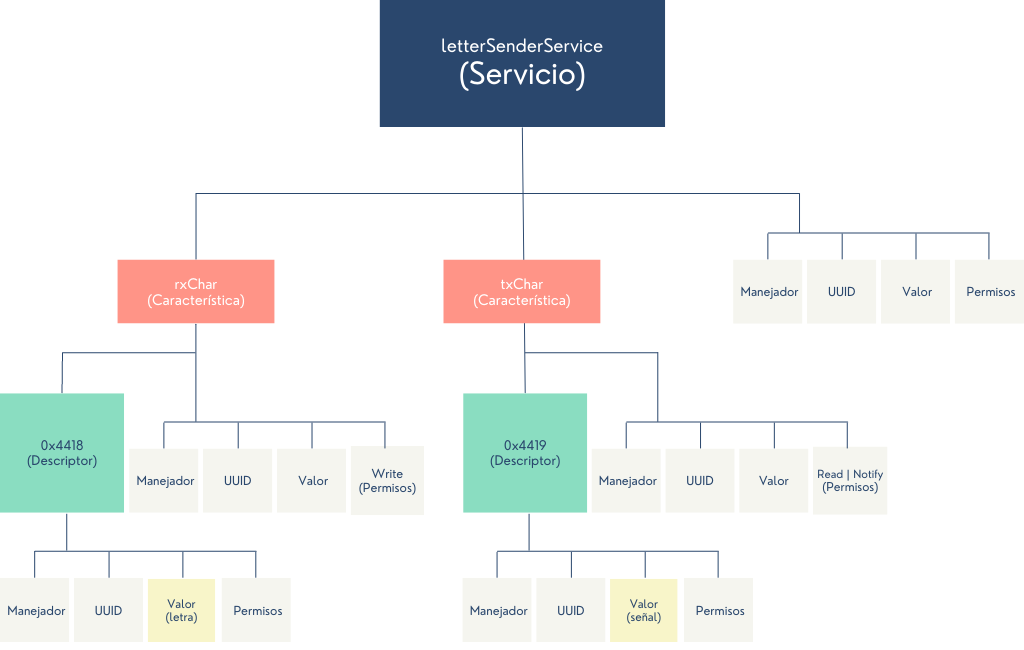
\includegraphics[width=1\textwidth]{capturas/BleLetterSenderService.png}\\[-0,40cm]
    \caption{Esquema de la estructura planteada para el servicio \textit{BLE}}
\end{figure}

\section{Implementación}
Previo a la implementación del código, se deben instalar ciertas librerías
(proceso sencillo gracias a la decisión de utilizar el \textit{Arduino IDE}
pero que puede consultarse en el apéndice \ref{libArduino})
para el trabajo con algunas características de la \textit{Arduino Nano Sense 33 BLE}
como lo son la librería \textit{Arduino\_LSM9DS1}, para el uso de la IMU y su
acelerómetro, magnetómetro y giroscopio; y la librería \textit{ArduinoBLE},
para el uso del \textit{Bluetooth} de bajo consumo. Por otro lado, también
es necesario instalar la librería \textit{Arduino\_TensorFlowLite}, para
trabajar con el modelo de la red neuronal en el firmware del microcontrolador.

Además, en ocasiones, es necesario dar permisos al puerto del microcontrolador
como reza el \textit{apéndice \ref{pserie}}
\subsection{Definición de parámetros de \textit{Bluetooth}}
En el primer bloque del firmware, encontramos definición de los parametros
que más tarde se utilizarán para configurar el \textit{BLE}
(Bluetooth Low Energy)\textsuperscript{\cite{ladvien}}\label{paramBT}.

La configuración de permisos de las características son consecuentes con
su cometido. La característica de lectura, tendrá permisos de escritura
para que la \textit{central} pueda escribir los valores que la placa leerá.
Análogamente la característica de escritura tendrá permisos de lectura y
notificación.

\begin{teoria}{Roles de las partes en conexiones \textit{bluetooth}\textsuperscript{\cite{BLEOreilly}}}
    \color{mitexto}
    Al darse una conexión bluetooth, existen ciertas implicaciones inherentes
    a la propia conexión. Y es que siempre habrá una de las partes que
    se lucra de los servicios de la(s) otra(s).\\
    Pues bien, los dispositivos que se gestionan o se benefician de los
    servicios de otros, se conocen como \textit{central} y los que proveen,
    son los \textit{periféricos}.
\end{teoria}
El resultado de la configuración del servicio \textit{BLE} obedece completamente
al diseño planteado.

Finalmente se deben definir una serie de manejadores para gestionar los
distintos eventos relacionados con el servicio \textit{BLE}. Estos manejadores
se activarán como consecuencia de suceso y se encargarán de gestionar
la respuesta a dicho suceso; concretamente respuestas a conexiones,
desconexiones o recibo de señales por el canal de lectura \textit{rx}.


\subsection{Función de configuración del firmware}
En esta sección (denominada función '\textit{setup()}' en el diseño de \textit{Arduino}),
como de constumbre, se deberá llevar a cabo el ajuste propio para la ejecución
de nuestro código\textsuperscript{\cite{andriyadimw}\cite{petewardenmw}}.

Es reseñable mencionar que el microcontrolador con el que estamos trabajando solo
posee la \textit{memoria flash} y \textit{SRAM} características de
los dispositivos de estas prestaciones. Sin embargo tenemos que almacenar
alguna información imprescindible como la red neuronal o la reserva de algunas
secciones de memoria. Para ver la solución implementada con un mayor detalle técnico,
consultar el apéndice \ref{memFlash}.
Más adelante se hará uso de la misma técnica para resolver el problema
de la integración de la red neuronal en el microcontrolador, entre otros.

\subsubsection{Configuración \textit{Bluetooth} y de sensores}
En esta primera etapa de configuración, se definirá el comportamiento de algunas
características de la placa; en primer lugar, el de la  \textit{IMU}
(\textit{Inertial Measurement Unit}), la unidad con la que trabajamos para
obtener los datos del movimiento sirviéndose de un \textit{giroscopio} y un
\textit{acelerómetro}, y por otro lado, la configuración del ya descrito,
definido y diseñado \textit{BLE} (\textit{Bluetooth Low Energy}) con
los parámetros que se definieron en la sección \ref{paramBT}.
\begin{teoria}{Por qué es necesario configurar la \textit{IMU}\textsuperscript{\cite{imuteoria}}}
    La \textit{IMU} es una parte fundamental de este proyecto, ya que es
    el dispositivo contenido en la placa que gestiona las mediciones de
    aceleración y velocidad del movimiento y que consta para ello de
    acelerómetro y giroscopio. Con la captura de estos datos, podrá rasterizarse
    una imagen que contenga el trazo descrito y con la que podremos alimentar
    la red neuronal.
\end{teoria}

\begin{problemas}{Librería Arduino\_LSM9DS1}
    \color{mitexto}
    Uno de los problemas con esta parte del código, fue que
    la librería \textit{Arduino\_LSM9DS1} necesaria para poder trabajar con
    la \textit{IMU}, tiene varias versiones.
    Al haber leído para algunos de los proyectos TFLite de
    arduino, que era recomendable utilizar su primera versión, fue la elegida.
    Sin embargo esta primera versión, no posee una de las funciones
    necesarias para trabajar con la \textit{IMU} en nuestro caso,
    que es el llenado
    contínuo de la FIFO de lectura de medidas recogidas, que por defecto
    funciona en \textit{oneShotMode}, es decir, llenado a ráfagas.
    Es necesario poder disponer de la función para trabajar en tiempo
    real con la predicción de letras y también es imprescindible para la
    recolección de muestras, como se verá más adelante.
    
    Por lo que la solución es o bien añadir manualmente la función en la
    librería, o bien actualizarla a la versión \textit{1.1.0}. Yo me he
    decantado por actualizar la librería, ya que es algo más limpio que
    editar una librería que no has programado tú mismo.
\end{problemas}

Por lo que solo resta fijar los parámetros creados para \textit{BLE},
vincular sus señales con manejadores de los eventos y hacer lo propio
con la \textit{IMU}.

Cabe destacar que adicional a la configuración \textit{BLE} descrita, también
se incorpora otro servicio con la característica \textit{strokeCharacteristic},
menos interesante de explicar, ya que utilizaré el método de recolección de
muestras de \textit{Pete Warden} para uno de los ejemplos
\textit{TFLite de Arduino}: \textit{magic\_wand}\textsuperscript{\cite{petewardenmw}}.

\subsubsection{Configuración para la red neuronal}
Parte de máxima trascendencia, ya que, es imprescindible configurar de
manera adecuada los parámetros del modelo para que el reconocimiento
se de manera óptima.\\
Una vez obtenemos el modelo definido en \textit{deep\_pen\_model\_data.cpp},
proceso que se explicará en la sección \ref{RNenμC}.

Se deben establecer las micro-operaciones que se darán en el modelo
para tener definido el repertorio en tiempo de ejecución que utilizará
nuestro interprete\textsuperscript{\cite{intro-tensor-micro}}.
Existe una alternativa que añade todas las micro-operaciones de forma genérica,
a costa de un mayor uso de memoria. Para mayor profundización de la
implementación, consultar el apéndice \ref{firmwMO}.

\begin{problemas}{Al cargar el firmware\, la placa deja de ser detectada}
    En las primeras cargas del firmware experimentando con el modelo, la placa
    dejaba de ser detectada. Lo primero que pensé es que el bootloader se había
    bloqueado. Sin embargo al restaurar la placa manualmente ({\small Pulsación
    del botón reset justo al conectar la placa}), el 'L' led de la placa,
    comenzó a parpadear; indicativo de que la placa se había restaurado.
    Por tanto solo cabía que el programa cargado era erróneo.
    Dado que tanto la compilación como la ejecución no informaban de errores,
    fue complicado dar con que este error se debía a una mala configuración
    de las microoperaciones definidas.\\Ya que al hacer cambios en el diseño
    del modelo, es imperativo añadir las microoperaciones ampliadas.
    Un error de principiante que llevó mucho tiempo arreglar.
\end{problemas}

Para finalizar la configuración de \textit{TensorFlow Lite} definimos el interprete del modelo, que hará
uso del repertorio de micro-operaciones especificadas.\newline
Y por último, inicializamos los led pins como salida, para poder hacer uso
del led como indicativo de estado.

\subsection{Función cíclica del firmware\textsuperscript{\cite{andriyadimw,petewardenmw}}}
En esta función (denominada 'loop()' en el diseño \textit{Arduino}),
será donde se establezca el código que se ejecutará persistentemente
mientras la placa esté alimentada.

En primer lugar, se tratará la lógica para los leds es simple:
\begin{figure}[h]
    \centering
    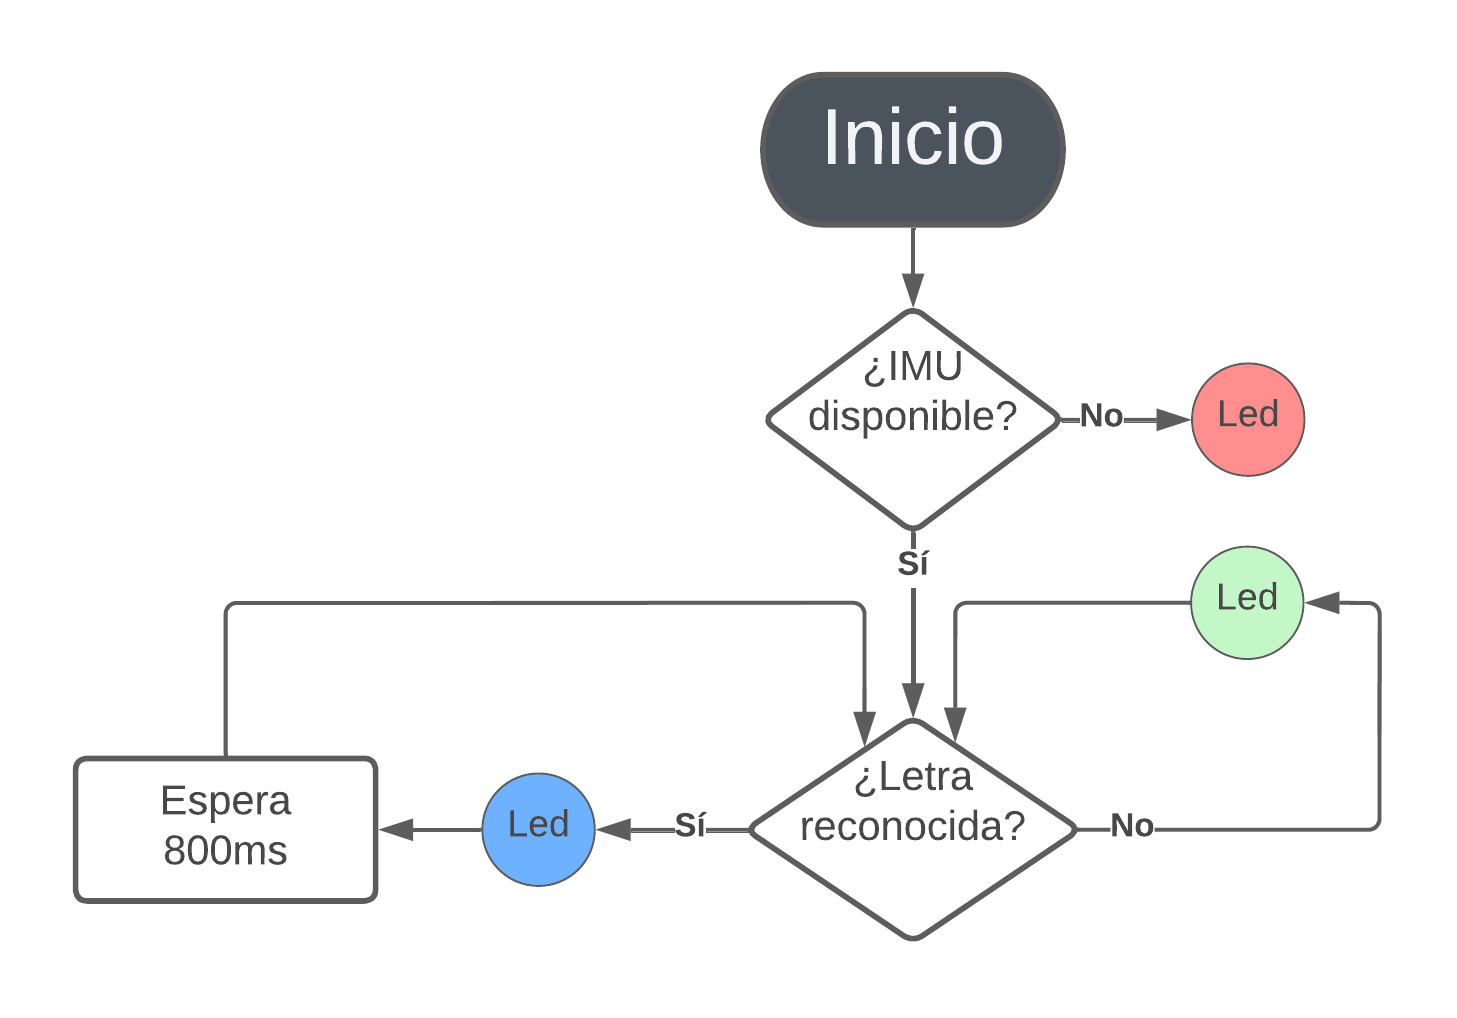
\includegraphics[width=0.82\textwidth]{capturas/DiagramaFlujoLeds.png}\\[-0,20cm]
    \caption{Diagrama de flujo de leds}
\end{figure}\\
En estado idle el led
encendido será el verde y en estado de detección de letra, será azul (quedará en este estado
durante 800ms, tiempo durante el que no se detectará nada, para que el usuario pueda
reposicionar su postura para volver a escribir otra letra); en caso de que la \textit{IMU}
no esté disponible, se encenderá el led rojo.

Para notificar una vez la conexión a un dispositivo, pese a que
la ejecución es cíclica, se implementa una sencilla solución descrita en el
apéndice \ref{BTcon}.

En cuanto al registro de movimiento, se han utilizado algunas de las funciones
del trabajo de \textit{Pete Warden} y su \textit{magic\_wand}\textsuperscript{\cite{petewardenmw}}
a modo de librería para mi propio proyecto y así aligerar el desarrollo de
la recolección de trazos y su rasterización.

Durante este proceso, se hará uso del giroscopio para determinar los cambios del trazo y el acelerometro
para pequeños ajustes sobre los resultados obtenidos con el giroscopio, por ejemplo
cálculos de gravedad y parámetros de velocidad del cambio de trayectoria del trazo.
Gracias a contar con las funciones antes citadas, tomar los valores de los sensores
es tan fácil como llamar a la función \textit{ReadAccelerometerAndGyroscope}.
Con los valores leídos, se hace un pequeño arreglo de estimación de desvío del giroscopio
y se envían los valores leídos como característica del servicio para \textit{Data Collector},
donde se recogeran las muestras para entrenar la red neuronal.
Y con el trazo completamente construido y corregido, se rasteriza el movimiento para
obtener la imagen que pasará por el modelo.

Con todo lo anterior definido, todo está listo para dar comienzo con el procesamiento
en la red neuronal. Para llamar a su ejecución,
se invoca el interprete, que arrojará los resultados en un puntero anteriormente definido.
Este puntero de salida, contiene los datos asociados al tensor, es decir, el producto
de que el trazo rasterizado haya pasado por la red neuronal. En nuestro caso, lo que
se obtiene de la red neuronal, es una valoración de ajuste de afinidad del trazo rasterizado
a lo que el modelo ha sido entrenado para reconocer como letras (nuestros \textit{labels}).\
Sintetizando, lo que se obtiene como salida de la red neuronal, es una valoración
de semejanza a cada letra, codificada como un índice.

Por tanto, lo que resta es trivial, solo tenemos que obtener el \textit{label} con mayor valoración.
Y como consecuencia, la letra que el modelo ha estimado más posible respecto a su entrenamiento.

Obtenida la letra, es enviada al puerto serie, para cuando se trabaje con conexión física;
y se introduce en la característica de transferencia(\textit{tx}) para cuando se trabaje
con el servicio \textit{Bluetooth} (\textit{BLE}).

Como comprobación concluyente, se verifica si la característica de lectura (\textit{rx}) ha sido
escrita por el programa de usuario, suponiendo esto una señal de que ya ha sido leída la letra
actual en \textit{tx} y como consecuencia, haciendo que se restaure su valor a uno por defecto;
ya que de no hacerlo, la letra permanecería inmutable en la característica y el programa
de usuario leería las mismas letras reiteradamente hasta escribir otras.
Esto se debe a que el las \textit{características} en \textit{BLE} funcionan con valores
constantes hasta que se modifique el estado actual.

\begin{figure}[h]
    \centering
    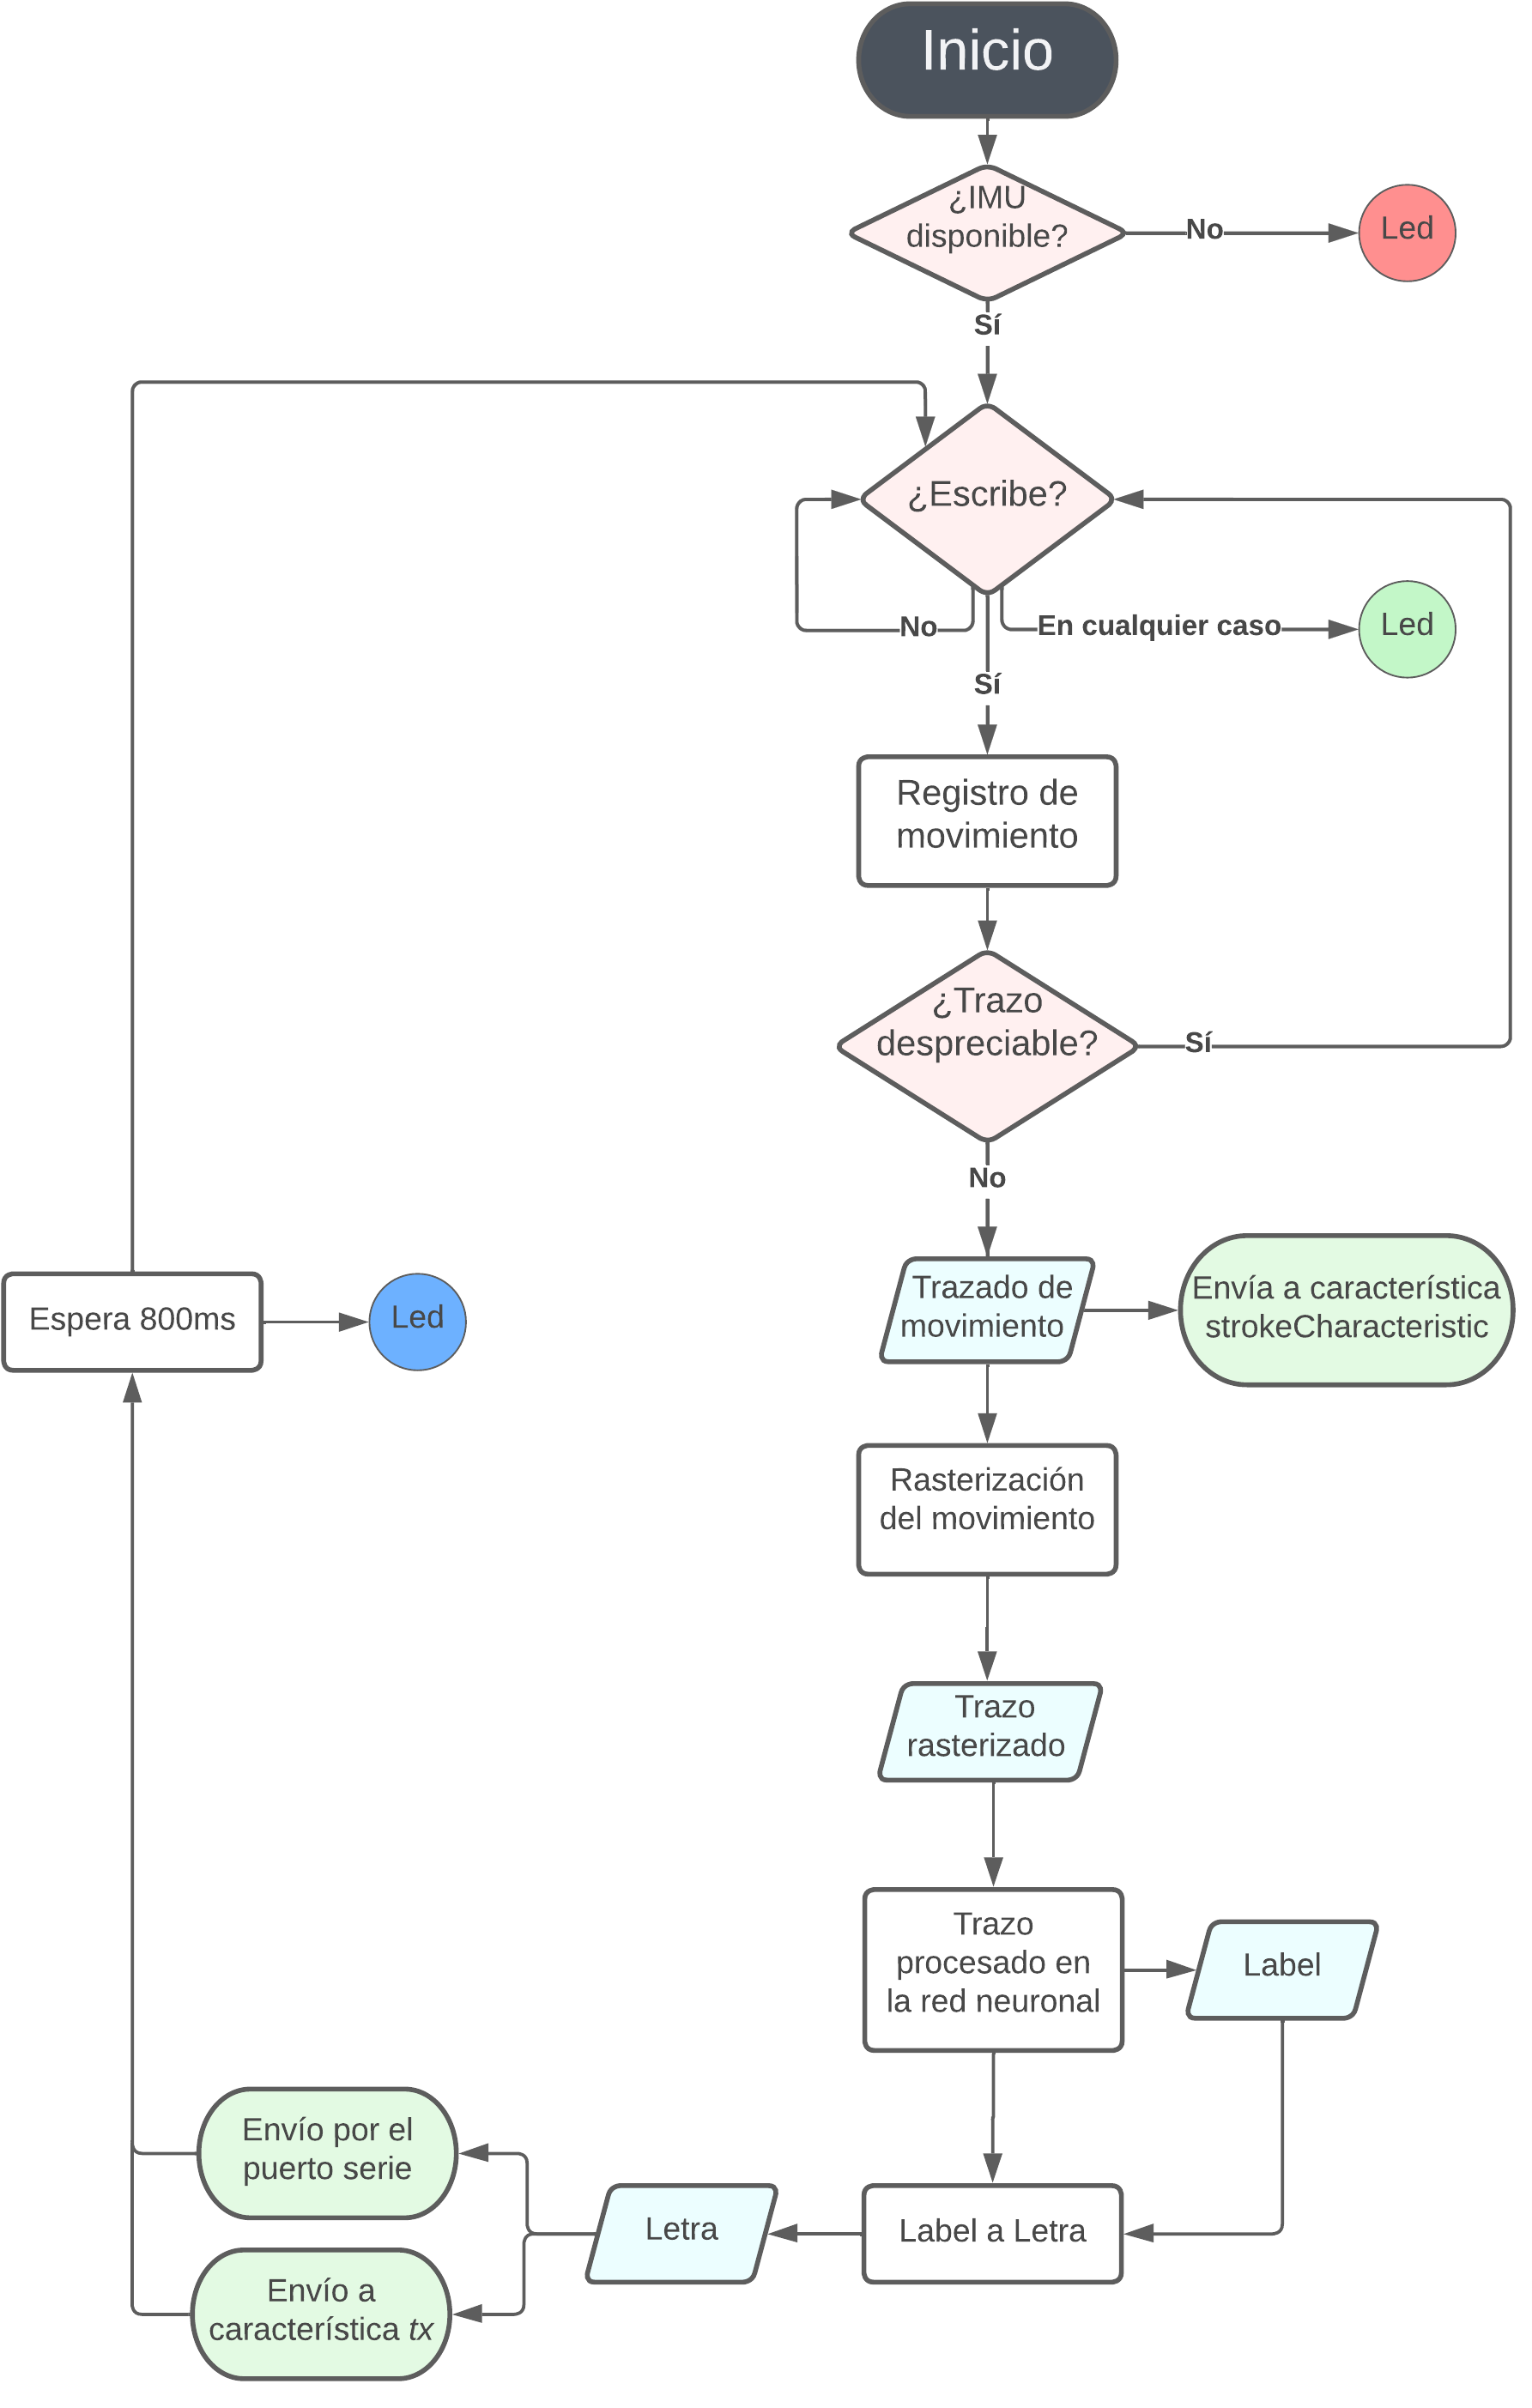
\includegraphics[width=0.8\textwidth]{capturas/DiagramaFlujoFirmware.png}\\[-0,48cm]
    \caption{Diagrama de flujo simplificado del firmware del microcontrolador}
\end{figure}

	% Diseño y entrenamiento de la red neuronal
	\chapter{Red Neuronal}

\section{Planificación}
\subsection{Elección de framework y librerías}
En esta sección se defenderá la elección de las herramientas utilizadas
para el desarrollo de la red neuronal, resultando una ampliación de la
\textit{sección \ref{fwDL}}, donde se ha tratado más la materia en términos
del modelo apartándonos de su integración en el microcontrolador.

\textit{TensorFlow Lite} se utilizará para la creación del modelo optimizado
para microcontroladores, pero esto no perturba en absoluto el desarrollo
ordinario en \textit{TensorFlow}. Es decir, se trabajará de igual forma
que si la red neuronal se utilizara en un equipo convencional, con la
única salvedad de la conversión del modelo ya generado a una versión optimizada
para microcontroladores; así es la dinámica de trabajo con \textit{TinyML}.

Como complemento a \textit{TensorFlow} y para facilitar el desarrollo de la
red neuronal, se empleará \textit{Keras}, una \textit{API} de alto nivel
que, desde hace unos años, pertenece a \textit{TensorFlow}; sirviendo para
actuar como interfaz a nivel de capa para \textit{TensorFlow}, o expuesto de
otra forma, facilita el desarrollo al simplificar el trabajo con las capas
del modelo. Además también se utilizará para el estudio de los resultados
del entrenamiento.

Como entorno de desarrollo, se utilizará \textit{Google Colab}, se podrían
emplear alternativas que se ejecutan localmente como \textit{PyCharm},
\textit{Jupyter} o \textit{Eclipse}; sin embargo con \textit{Google Colab}
podemos aprovechar la capacidad de cómputo de sus \textit{GPU}s, lo cual agiliza
mucho los tiempos de \textit{entrenamiento} y \textit{validación}. Si bien,
el tiempo de uso del que se dispone de estas \textit{GPU}s, es limitado, aunque
siempre podemos continuar haciendo uso de las \textit{CPU}s. Además, al tratarse
de una alternativa en la nube, la etapa de configuración es mínima: apenas
instalando las librerías de las que vamos a hacer uso, ya tenemos desplegado
el entorno de trabajo.


\subsection{Diseño de la red neuronal}
El diseño de un modelo es determinante para que se desenvuelva apropiadamente
a la hora de realizar su función. Por más que se dote al modelo durante el
entrenamiento de un gran volumen de datos, será vano si el diseño no está enfocado
a la labor que tiene que desempeñar. Por lo tanto, para el diseño de este modelo,
se han estudiado otros muchos de clasificación de formas y procesamiento de imagen; la
mayoría hacían uso del célebre \textit{MNIST}: una base de datos que cuenta con
60.000 imágenes de entrenamiento y 10.000 de testeo, es un gran dataset de imágenes
de dígitos. Aunque en general se han consultado todo tipo de modelos para el
procesamiento de imágenes y clasificación, destacando el referente de este proyecto
\textit{Magic Wand}\textsuperscript{\cite{petewardenmw}} de \textit{Pete Warden}.
Para examinar con mayor profundidad la experimentación respecto al diseño del modelo,
observese el \textit{apéndice \ref{expRN}}.

El modelo que mejor funciona y más se utiliza en trabajos simples de procesamiento
de imagen para clasificación, es el de \textit{redes neuronales convolucionales}
(\textit{CNN}); definidas en una estructura muy marcada como ya se describió
en la Figura \ref{cnn}.
\begin{teoria}{Redes neuronales convolucionales}
Estas \textit{redes neuronales convolucionales}
no son más que un tipo de red neuronal que, reduciendo a un nivel muy básico,
utiliza un tipo de capa que realiza una operación matemática llamada convolución.

Lo cual nos lleva al siguiente paso, la definición de convolución: operador
matemático que haciendo uso de dos funciones $f$ y $g$, genera una nueva
a partir de estas, que representa la magnitud de su superposición.
Concretamente en 2 dimensiones, podemos entenderlo, tal y como ilustra la
Figura \ref{conv2d} como el producto del \textit{kernel} o \textit{filtro}
y una subventana de la matriz, generalmente una imagen; al repetir este producto
para todas las subventanas, obtenemos una nueva matriz resultado de la convolución.

Encontrar los valores del \textit{kernel} y por tanto la magnitud resultante
del análisis de la imagen de entrada, será la principal labor de la capa de
convolución.

Al resultado de la convolución, se le denomina \textit{mapa de características},
y su función es evidenciar dónde se encuentra la característica buscada por el
\textit{kernel}. Estos \textit{mapas de características} pueden reflejar
cambios de contraste, texturas, superficies planas, etc.

Pues bien, la red neuronal realizará esta operación secuencialmente, es decir,
el resultado de una capa, alimentará a la siguiente. Lo cual provoca que,
unido a un proceso de \textit{agrupación}, cada vez la información relevante
se condense y refine más y más, permitiendo extraer patrones cada vez más
complejos.
\end{teoria}\newpage

\begin{figure}[h]
    \centering
    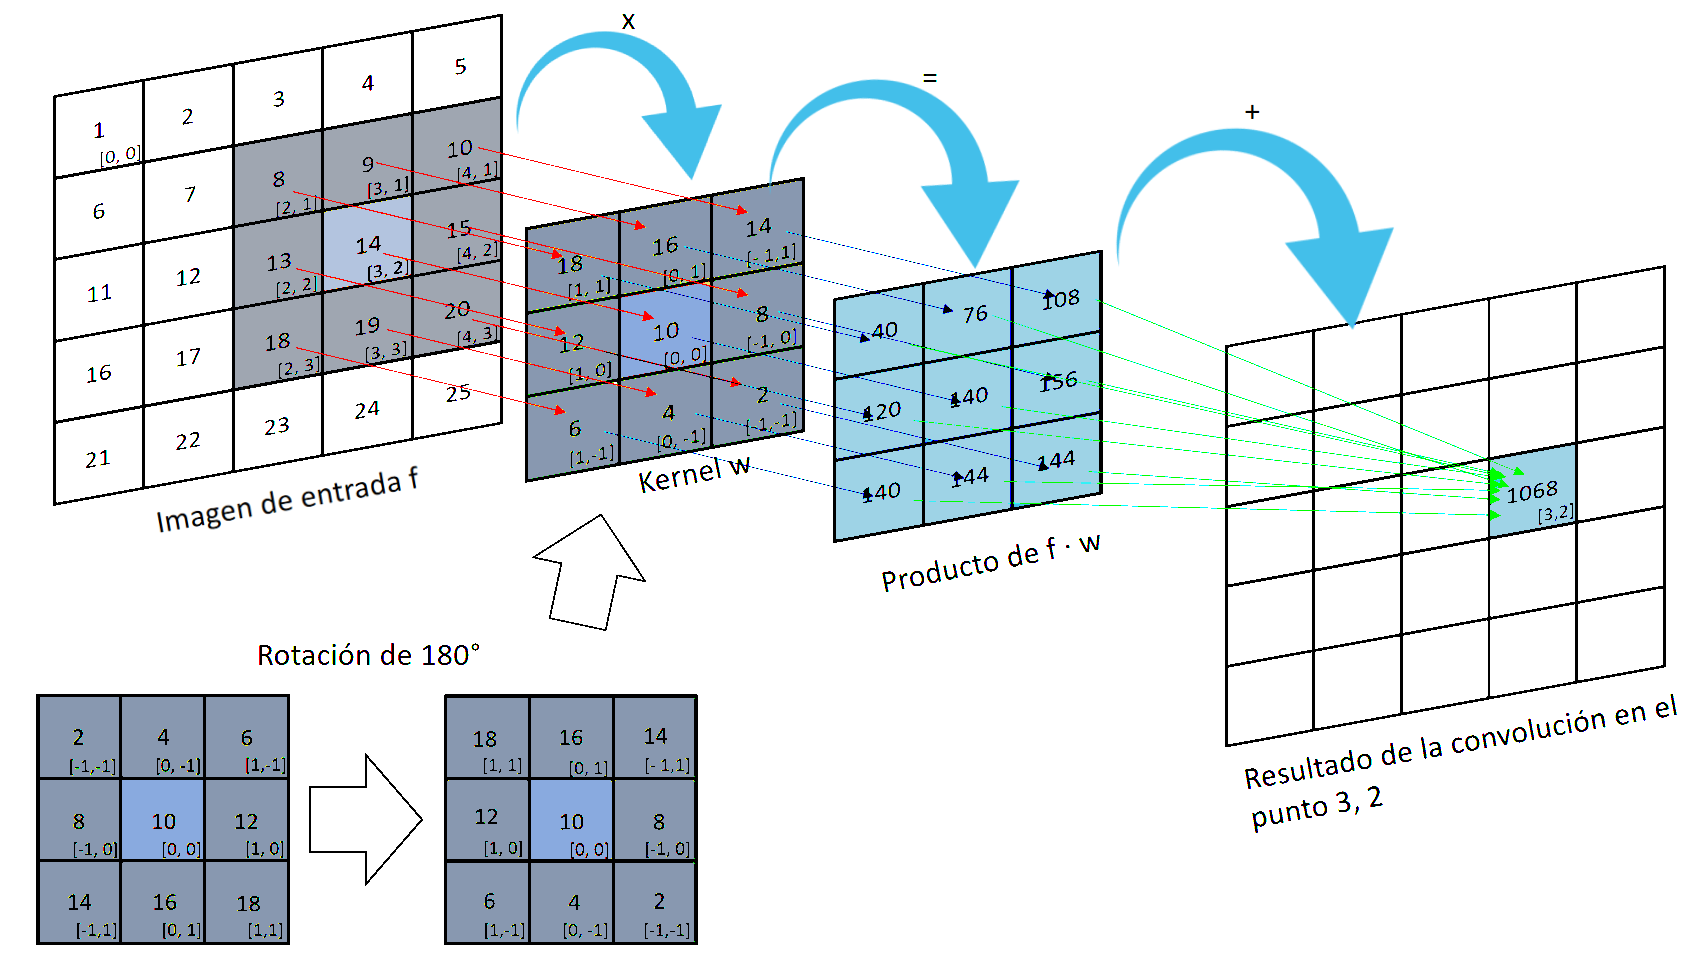
\includegraphics[width=1\textwidth]{capturas/conv2D.png}\\[-0,40cm]
    \caption{Esquema de convolución 2D\label{conv2d}
    {\scriptsize (\url{https://bryanmed.github.io/conv2d/})}}
\end{figure}

Conociendo la teoría de la \textit{red neuronal convolucional}, 
ya es posible comentar el diseño concreto implementado.
El modelo cuenta con una estructura de
\textit{Sequential} de \textit{Keras};
gracias a esta utilidad, es posible añadir capas al modelo de forma cómoda, además
de permitir el acceso a algunas funciones para el entrenamiento.
Se describirá la estructura en términos generales, para encontrar una descripción
a nivel de implementación real con \textit{Keras}, véase el \textit{apéndice
\ref{capasKeras}}

El modelo utilizado va a contar con tres bloques de procesamiento tras la entrada,
formados por una capa de \textit{convolución}, otra de \textit{normalización}, \textit{activación} y \textit{fropout}.
Estos bloques deben su composición a que el aporte de cada una de las capas,
complementa al procesamiento convolucional, en el caso de nuestro modelo, que
trabaja con imágenes tan pequeñas, son prácticamente irremplazables.
Comenzando por la inherente capa de \textit{convolución}, donde se dará el
procesamiento anteriormente ilustrado. Tras esta, se normaliza la salida mediante una capa
para este propósito, lo cual garantiza una mayor estabilidad y eficiencia
en el proceso de aprendizaje. Se define como función de activación, \textit{relu}; no
por otra cosa que porque es la más utilizada, la que mejor funciona para prácticamente
todas las labores sin tener que profundizar en el estudio del mismo y por su bajo
coste computacional; destacable debido a la naturaleza del dispositivo en el que
se ejecutará la red neuronal. Y por último la capa de \textit{Dropout} para mitigar
el overfitting, un problema que se ha podido experimentar debido a que es una red
neuronal de reducida complejidad.

En cada uno de los tres bloques, lo único que varía es el número de filtros de
la capa de convolución, duplicándose respecto al anterior.

Comentada la estructuración de estos bloques y su fundamento, ya es posible
desarrollar el modelo completo.
Al inicio, preliminar a los tres bloques citados, hay una capa de \textit{reescalado},
que va a servir meramente para normalizar los valores los píxeles de las imágenes
a una escala [0,1].
Tras esta, se encuentran los tres bloques descritos y posterior a estos,
una capa de \textit{agrupación} por simple
coherencia estructural debido a que reduce la dimensionalidad pero conserva la mayor
parte de información relevante (utilizada en la práctica totalidad de \textit{CNN}s).
Otra capa \textit{dropout} por el mismo motivo que en los
bloques y finalmente una capa densa \textit{softmax} con la que obtendremos una distribución
de probabilidad y así adquirir un output clasificatorio del mismo tamaño que número de letras
reconoce la red neuronal. Toda esta arquitectura se ilustra, simplificada, en la Figura \ref{esqRN}.

\begin{figure}[h]
    \centering
    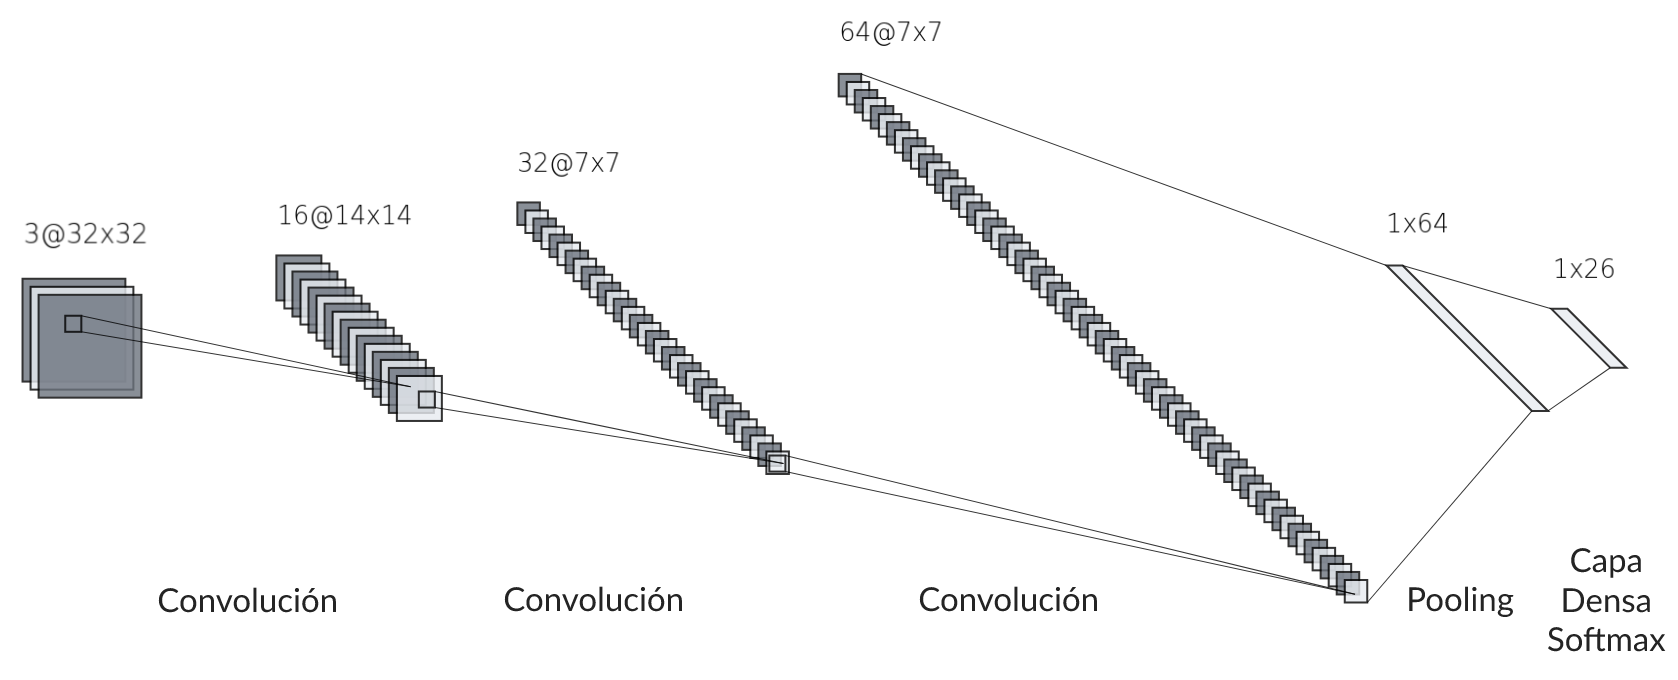
\includegraphics[width=1\textwidth]{capturas/esquemaRN.png}\\[-0,40cm]
    \caption{Esquema de la red neuronal diseñada \label{esqRN}}
\end{figure}

\section{Implementación}
\subsection{Preparativos}
Previo al diseño, se han de instalar ciertas dependencias y definir
algunos parámetros asistentes para el código. La mayoría de dependencias
son para trabajar con estructuras de datos en python, interfaces con el OS, o
librerías para \textit{TensorFlow} y \textit{Keras}.
También se ha hecho uso de algunas funciones del trabajo de
\textit{Pete Warden}\textsuperscript{\cite{petewardenmw}}.

Otra dependencia imprescindible es \textit{xxd}.
\begin{teoria}{Uso de \textit{xxd}\textsuperscript{\cite{tf-xxd}}}
    \color{mitexto}
    Es esencial contar con \textit{xxd}, esto se debe a que la mayoría de
    microcontroladores no tienen soporte para sistema de archivos nativo.
    Con \textit{xxd} obtenemos el modelo en formato matriz de chars directamente
    compatible con \textbf{C/C++} e integrable en cualquier microcontrolador.\newline
    Es recomendable establecer esta matriz como constante por cuestiones de
    eficiencia en el acceso a memoria.
\end{teoria}
\newpage

También necesitaremos el dataset para el entrenamiento, validación y testeo
del modelo. Se ha decidido que en pos de la experimentación y de un mejor desempeño
de la red neuronal al entrenarla con muestras generadas de la misma forma que se generarán
las que se procesen cuando se haga uso de esta en el microcontrolador; que se generarán
las muestras que utilizaremos como dataset, es decir, se va a generar un dataset propio.
Este datase se irá
actualizando a medida que se toman más muestras y que se podrá descargar
desde el \textit{Google Drive} institucional. Se acompaña la descarga de una comprobación
de existencia del fichero descargado para concluir esta sección.

Con el dataset descargado, se almacenan los trazos en un array, en el que
cada elemento del array será un trazo; de momento de todos los labels.

Los trazos en este momento están cargados como conjunto de coordenadas que
conforman, unas seguidas de otras, un recorrido; presumiblemente una letra.
Pero como ya es sabido, nuestro modelo necesita como entrada imágenes; por lo que
el siguiente paso es rasterizar los trazos para producir una imagen.

Al igual que en el firmware del microcontrolador, se hará uso de la función de rasterización creada
por \textit{Pete Warden}\textsuperscript{\cite{petewardenmw}}. Definidas las funciones de
rasterización, es posible rasterizar todos los trazos del dataset y destinarlos a las distintas
fases del desarrollo del modelo como se verá en las siguientes secciones.

{\color{red}Hablar de bloque 'PREPARE DATASETS'}

\subsection{Entrenamiento}
El entrenamiento del modelo será el segundo puntal que, junto con el diseño del
propio modelo, dotará de estabilidad a nuestra red neuronal; siendo ambas dos
determinantes para que esta responda de forma óptima a la tarea para la que a
la que ha sido dispuesta.
Por lo que la configuración del entrenamiento debe ser lo mejor posible, ajustando
\textit{epochs} (iteraciones en el proceso de entrenamiento), \textit{learning\_rate}
(escalabilidad del aprendizaje), \textit{optimizadores}, etc.
Para ver el ajuste experimental de estos valores, véase el \textit{apéndice \ref{expRN}}.

Las imágenes de los datasets ocuparán 32x32 píxeles. Este es otro parámentro que puede
ser estudiado, no obstante, estas dimensiones han sido las que han arrojado mejores
resultados de forma homogénea. Como de costumbre, para más información a este respecto,
consultar el \textit{apéndice \ref{expTrainRN}}.

Se utilizará el mismo conjunto de datos aleatoriamente distribuido para cada
uno de los tres dataset. Cada dataset contará con un porcentaje del conjunto de datos
total. Estos porcentajes han sido estudiados y a priori no suponen extrema relevancia
más allá de que el de entrenamiento debe ser ampliamente mayor. Ha sido fijado un
10\% para test, otro 10\% para validación y el restante 80\% para entrenamiento.
\newpage
\begin{teoria}{Uso del dataset en \textit{Deep Learing}(1)\textsuperscript{\cite{Andreas}}}
    \color{mitexto}
    Los tres datasets que se usan para \textit{Deep Learing} son:
    \begin{itemize}
        \itemsep0em
        \item \textbf{Validation}\\
        {\small En \textit{Deep Learning} se usan datos de validación para corroborar
        durante el entrenamiento, que el ajuste se está dando de forma óptima.\newline
        Dilatando un poco más esta sencilla explicación, el \textit{validation dataset}
        es un conjunto de datos imperativamente distinto del \textit{training dataset},
        que sirve para estimar la eficacia de la red en tiempo de entrenamiento.\newline
        En general se suele usar la validación para hacer estudios del ajuste del modelo,
        para evitar sobreajustes (\textit{overfitting}) y subajustes (\textit{underfitting}).}
        \begin{teoria}{\textit{Overfitting} y \textit{Underfitting}\label{ovYun}}
            \color{mitexto}
            \begin{itemize}
                \item \textbf{\textit{Overfitting}}\\
                {\small Es un fenómeno que se da cuando el modelo reconoce peculiaridades
                demasiado específicas como distintivo para la evaluación. Estas
                peculiaridades no serían los rasgos o características que constituyen
                a los elementos que estudiados y por lo tanto se produce un
                sobreajuste; un ajuste por encima de lo óptimo.} 
                \item \textbf{\textit{Underfitting}}\\
                {\small Término análogo y opuesto al anterior, el ajuste se
                presentaría laxo y falto de rigurosidad; ajuste por debajo de
                lo óptimo.} 
            \end{itemize}\end{teoria}
        \item \textbf{Training}\\
        {\small Este dataset es el más simple de entender por mera inmediación
        semántica. Es el conjunto de datos que se utiliza en tiempo de entrenamiento
        para balancear los pesos de las capas. En cada iteración de entrenamiento,
        se calcula la pérdida con los datos de entrenamiento introducidos y
        se da el ajuste de pesos en base a la pérdida. Esto supone que, cada vez la
        pérdida sea menor y generalmente la eficacia, o en términos más comunes a este
        ámbito, la \textit{precisión} (\textit{accuracy}), sea mayor.}
        \item \textbf{Test}\\
        {\small El conjunto de datos que se utilizará posterior al entrenamiento, para
        validar la efectividad del entrenamiento.
        Es el dataset con el que se pone a prueba el modelo entrenado.}
    \end{itemize}
\end{teoria}
\newpage

\subsection{Testeo}
El testeo del modelo es útil para garantizar que funciona correctamente, sin
embargo podemos obtener valores muy buenos sin resultar en un funcionamiento
adecuado, debido al ya mencionado \textit{overfitting} (\textit{Teoría \ref{ovYun}}).
Por tanto solo debemos tomarlo como una herramienta más, siempre evaluando
adecuadamente los resultados.

La fase de testeo consiste en simular lo que será una ejecución habitual,
pero conociendo los inputs de la red neuronal, que serán del dataset
de testeo. Obteniendo imágenes de cada letra (\textit{label}), se evalúa
la clasificación de la red neuronal de la misma, junto con la precisión
de estimación; si la clasficación coincide y además lo hace con valores de
precisión próximos a 1, significará, en principio, un buen desempeño de la red
neuronal para
esta letra. El objetivo es conseguir esto para todas las letras.

Es importante separar los dataset de testeo de los de entrenamiento
y validación, ya que si se emplearan los mismos, el modelo ha sido entrenado
con este mismo input, por tanto siempre se obtendrían buenos resultados
y el testeo perdería validez.

Para un mayor acercamiento a la experimentación con el testeo de los modelos
probados, visite el \textit{apéndice \ref{expTrainRN}}

\subsection{Transformación a modelo cuantizado}
El hecho de cuantizar el modelo basado en \textit{Deep Learning} cuando se
plantea su integración en microcontroladores y equipos de bajo rendimiento,
suele ser imperativo.

\begin{teoria}{Cuantización}
    \color{mitexto}
    Cuantizar es desvirtuar la naturaleza continua de un conjunto de valores continuos,
    restringiéndolos a un conjunto de valores discretos.
\end{teoria}

En general esta práctica viene propiciada debido a que
la mayoría de microcontroladores no cuentan con \textit{FPU}
(\textit{Floating Point Unit}). Sin embargo no es este el caso, ya que en este
proyecto se escogió un microcontrolador que sí dispone de esta unidad. Aun
así se ha tenido que recurrir a la cuantización del modelo, como consecuencia
de su limitación de memoria, ya que el hecho de cuantizar el modelo, supone
reducir su precisión y por tanto reducir la memoria que este requiere.

Sin entrar en muchos detalles, ya que es parte de la siguiente sección,
el modelo generado estándar queda muy lejos de poder integrarse en el
microcontrolador, gracias a la conversión a un modelo \textit{TensorFlow Lite},
se reduce el tamaño, pero sigue sin ser suficiente, por tanto es conveniente
cuantizar el modelo \textit{TensorFlow Lite} para obtener su
versión más compacta posible.


\subsection{Comparación de modelos generados}
Los modelos generados para la red neuronal, se muestran en la Tabla \ref{tabModelos}.
\begin{table}[h]
    \color{mitexto}
    \begin{tabular}{llll}
    \rowcolor[HTML]{6C737E} 
    {\color[HTML]{EFEFEF} \textbf{Modelo}}     & {\color[HTML]{EFEFEF} \textbf{Tamaño}} & \cellcolor[HTML]{6C737E}{\color[HTML]{EFEFEF} \textbf{Reducción TF}} & \cellcolor[HTML]{6C737E}{\color[HTML]{EFEFEF} \textbf{Reducción TFLite}} \\
    \rowcolor[HTML]{CDDADE} 
    TensorFlow                                 & 756009 Bytes~~                           & \cellcolor[HTML]{CDDADE}0\%                                          & \cellcolor[HTML]{CDDADE}-                                                \\
    \rowcolor[HTML]{E8ECF1} 
    TensorFlow Lite                            & 140300 Bytes~~                           & \cellcolor[HTML]{E8ECF1}81'4\%                                       & \cellcolor[HTML]{E8ECF1}0\%                                              \\
    \rowcolor[HTML]{CDDADE} 
    \cellcolor[HTML]{CDDADE}TF Lite cuantizado & 41136 Bytes~~                            & 94'5\%                                                               & 70'6\%                                                                  
    \end{tabular}
    \caption{Tabla de comparación de modelos generados\label{tabModelos}}
\end{table}

Los resultados son impresionantes en sí mismos, pero lo son aún más cuando ponemos
en contexto los valores de precisión que se alcanzan para cada uno de ellos en
la clasificación; variando en el peor de los casos del orden de 0,1\% de
\textit{TensorFlow} a \textit{TensorFlow Lite} y del orden de 0,2\% de
\textit{TensorFlow} a \textit{TensorFlow Lite} cuantizado.
Por lo que la compactación del modelo no tiene un impacto notorio
durante su ejecución.

\subsection{Integración en el microcontrolador\label{RNenμC}}
Esta sección sirve ahora a modo de recopilación de las anteriores,
ya que el procedimiento prácticamente ha sido expuesto.

La cuantización del modelo para optimizar el uso de memoria es el primer
paso; una vez el modelo cuenta con un tamaño apto para el microcontrolador,
lo que resta es solucionar el problema de la carencia de sistema de archivos
necesario para el manejo de la red neuronal construida con \textit{TensorFlow}.
Para lo cual se hace uso de \textit{xxd}, herramienta que automatiza el proceso
de conversión del modelo a una estructura de datos (\textit{vector} de
\textit{chars}), agregable al firmware del microcontrolador.

Cuando pasamos el modelo por \textit{xxd} y obtenemos el código en \textit{C},
es suficiente con añadirlo al código del \textit{firmware} y este ya es funcional
en el microcontrolador. Con el que se trabajará gracias a las librerías de
\textit{TensorFlow Lite}.

\section{Generación de muestras para el dataset\label{dataColl}}
Por suerte se podremos contar con una herramienta creada por
\textit{Pete Warden}\textsuperscript{\cite{petewardenmw}} para tomar
muestras de trazados con el microcontrolador que estamos empleando.
Se ha modificado superficialmente y se han hecho algunos cambios
estéticos (\href{https://github.com/AntonioPriego/SmartPen/blob/main/DataCollector/SmartPen_DataCollector.html}{DataCollector.html}). 
Este proceso supone, para el sujeto que genera las muestras, un tiempo de
adaptación al movimiento que se debe ejecutar para que se recoja un buen trazado,
añadido al hecho de que las muestras que no sean óptimas, deben eliminarse;
lo convierten en un proceso cargante y lento para quien está creando las muestras
y para quien tiene que supervisarlas.

A lo largo de la toma de muestras se han detectado ciertos fallos que
se han resuelto y son consultables en los Apéndices \ref{PWchrome},
\ref{borrarMuestras} y \ref{borraIndices}.

	% Diseño interfaz de usuario 
	\chapter{Interfaz de usuario}
\section{Motivación\label{justifUI}}
Antes de comenzar con la planificación, debe ponerse en valor la conveniencia
de esta interfaz de usuario. El principal motivo es que lo que se busca
con este proyecto es crear un producto real, y como tal, no podemos valernos
de un simple lector de puerto serie para el dispositivo, como podría ser
el integrado en el \textit{Arduino IDE}. Además, esta interfaz no solo está
creada con la funcionalidad de este proyecto en mente de servir de mediador
con el usuario para la lectura de las letras escritas con el \textit{SmartPen},
sino que busca ser el nexo de unión de todas las funcionalidades que se
implementen para este. Durante el propio desarrollo de esta interfaz, se
ha reflexionado sobre ciertas funcionalidades, como la de un modo pizarra
donde reflejar el trazado íntegro que se realice, y que se ha propuesto
finalmente como una meta secundaria.

\section{Planificación}
En esta sección se recogerán los motivos por los que se necesita de esta interfaz
de usuario, la elección de herramientas para su desarrollo y el bocetado de la distribución
de sus elementos.

\subsection{Elección de framework para interfaz gráfica}
Las alternativas con las que vamos a partir, tras una fase de documentación sobre
frameworks para desarrollo de interfaces gráficas, preferiblemente multiplataforma,
y sumarlas a las que ya conocía; se recogen en la Tabla \ref{tabUI}, junto a la valoración
de algunas características importantes.
\begin{table}[h]
    \color{mitexto}
    \begin{tabular}{|l|c|c|c|c|c|c|}
    \hline
    \rowcolor[HTML]{6C737E} 
    \cellcolor[HTML]{6C737E}{\color[HTML]{EFEFEF} \rotatebox{291}{\textbf{Alternativas}}} & \cellcolor[HTML]{6C737E}{\color[HTML]{EFEFEF} \rotatebox{291}{\textbf{Documentación}}} & {\color[HTML]{EFEFEF} \rotatebox{291}{\textbf{Usada anteriormente}}} & {\color[HTML]{EFEFEF} \rotatebox{291}{\textbf{Comunidad}}} & {\color[HTML]{EFEFEF} \rotatebox{291}{\textbf{Soporte para BLE}}} & {\color[HTML]{EFEFEF} \rotatebox{291}{\textbf{Lectura P.Serie nativa~}}} & {\color[HTML]{EFEFEF} \rotatebox{291}{\textbf{Multiplataforma}}} \\ \hline
    \rowcolor[HTML]{C3D6DC} 
    Flutter                                                              & {\color[HTML]{4CDE4C} \cmark}                                               & {\color[HTML]{4CDE4C} \cmark}                                                     & {\color[HTML]{4CDE4C} \cmark}                                           & {\color[HTML]{4CDE4C} \cmark}                                                  & {\color[HTML]{4CDE4C} \cmark}                                                        & {\color[HTML]{4CDE4C} \cmark}                                                 \\
    \rowcolor[HTML]{E8ECF1} 
    GTK+                                                                 & {\color[HTML]{4CDE4C} \cmark}                                               & {\color[HTML]{9B9B9B} -}                                                                         & {\color[HTML]{4CDE4C} \cmark}                                           & {\color[HTML]{FD6864} \xmark}                                                  & {\color[HTML]{FD6864} \xmark}                                         & {\color[HTML]{4CDE4C} \cmark}                                                 \\
    \rowcolor[HTML]{C3D6DC} 
    QT                                                                   & {\color[HTML]{4CDE4C} \cmark}                                               & {\color[HTML]{4CDE4C} \cmark}                                                     & {\color[HTML]{4CDE4C} \cmark}                                           & {\color[HTML]{4CDE4C} \cmark}                                                  & {\color[HTML]{4CDE4C} \cmark}                                                        & {\color[HTML]{4CDE4C} \cmark}                                                 \\
    \rowcolor[HTML]{E8ECF1} 
    PyQT                                                                 & {\color[HTML]{4CDE4C} \cmark}                                               & {\color[HTML]{FD6864} \xmark}                                                     & {\color[HTML]{4CDE4C} \cmark}                                           & {\color[HTML]{4CDE4C} \cmark}                                                  & {\color[HTML]{4CDE4C} \cmark}                                                        & {\color[HTML]{4CDE4C} \cmark}                                                 \\
    \rowcolor[HTML]{C3D6DC} 
    Electron                                                             & {\color[HTML]{4CDE4C} \cmark}                                               & {\color[HTML]{FD6864} \xmark}                                                     & {\color[HTML]{4CDE4C} \cmark}                                           & {\color[HTML]{FD6864} \xmark}                                                  & {\color[HTML]{4CDE4C} \cmark}                                                        & {\color[HTML]{4CDE4C} \cmark}                                                 \\ \hline
    \end{tabular}
    \caption{Tabla de elección de \textit{frameworks} para desarrollo de \textit{UI}s\label{tabUI}}
\end{table}

\textit{Electron} y \textit{GTK} quedan descartados porque, si bien existen
procedimientos para poder gestionar \textit{Bluetooth Low Energy} con estos, no tienen
soporte nativo ni librerías para ello, por tanto, teniendo la posibilidad
de hacer uso de otros frameworks que faciliten esta tarea, es factible
descartar estas opciones.

Ante \textit{QT (C++)} y \textit{PyQT}, debido a que se ha trabajado anteriormente
con \textit{QT (C++)} y el tiempo de desarrollo disponible es un factor
limitante, es razonable excluir \textit{PyQT}.

Solo quedarían \textit{QT} y \textit{Flutter}, se ha escogido ante estas dos
posibilidades \textit{QT}
por dos razones. La primera razón es que \textit{Flutter} está más dirigido
a interfaces móviles. Y la segunda razón es que pese a haber trabajado con
ambas, a título personal, me encuentro más habituado a \textit{QT}.

Por lo que el framework seleccionado para realizar la interfaz de usuario,
será \textit{QT} ya que ofrece soporte para las tecnologías que en principio
van a utilizarse y porque es una herramienta con la que ya se ha trabajado
y esto resulta en un menor tiempo de documentación, causa de peso
por el tiempo tan ajustado.

\subsection{Diseño de la interfaz\label{diseUI}}
Para el bocetado de la interfaz previo a la implementación, se hará uso
de \textit{QT Design Studio}, herramienta de \textit{QT} para diseñar
interfaces.
En el bocetado de la interfaz se fijarán los elementos que la formarán
y su disposición procediendo razonadamente.
Para entender visualmente lo que se va a describir, puede examinar el \textit{apéndice
\ref{ifazUsu}}.


Como se ha razonado en la
Sección \ref{justifUI} anterior, queremos que este programa sea el
\textit{hub} de funcionalidades para el \textit{SmartPen}, por lo que
se hará uso de una barra lateral para acceder a estas. Queremos que
el protagonismo se encuentre en la funcionalidad, por lo que esta
barra lateral será desplegable, para reducir el tamaño que esta ocupe
en la interfaz. Alojará las funcionalidades y, dada la naturaleza académica
del proyecto, una sección sobre el desarrollador, para más información sobre
el trabajo.

Cada sección de la interfaz, se
mostrará en la pantalla central, quedando las barras superior y lateral,
constantemente a la vista ya que la barra lateral sirve para acceder
a otras secciones de la interfaz y la barra superior muestra información
vital.

Es necesario un indicador de conexión y un botón de conexión inalámbrica,
que se ubicarán a la derecha en la barra superior para evitar sobrecargar
la zona izquierda de la interfaz.

En los primeros bocetos se evidenciaba un vacío en la parte central de
la barra superior y también se echaba en falta saber qué pantalla se estaba
mostrando en cada momento, por lo que uniendo ambas carencias, se
solventó disponiendo un indicador de pantalla en dicha región. 

\section{Implementación\label{implemUI}}
En cuanto a la implementación software, al margen de aplicar el diseño
descrito en la Sección \ref{diseUI} anterior, los retos planteados
son principalmente dos.
El primero de ellos: la gestión simultánea de la lógica de la interfaz, la lectura
del puerto serie y la lectura de \textit{características} del servicio
\textit{Bluetooth Low Energy} (definido en la Sección \ref{servBLE}).
El segundo: la implementación de lectura, especialmente la lectura haciendo
uso del servicio \textit{Bluetooth}.

Para afrontarlos, se hará uso de tecnologías que nos proporciona el propio
\textit{framework}. Para gestionar simultáneamente varios procesos, es
posible hacer uso de \textit{hilos} (o \textit{threads}) gracias a los
\textit{QThread}s de \textit{QT}, que proveen de una clase para gestionar
\textit{hilos} independientemente del sistema. Por lo que crearemos un
hilo concurrente a la ejecución de la lógica de la interfaz, que se hará
cargo de los procedimientos de lectura, tanto \textit{Bluetooth} como del
puerto serie; la clase
\href{https://github.com/AntonioPriego/SmartPen/blob/main/SmartPenUI/readerthread.cpp}{\textit{ReaderThread}}.

Por otro lado, para resolver el problema de la lectura de la placa,
tanto la lectura por cable como la inalámbrica, se emplearán
librerías que asisten para estas tareas. Ya se planteó como requisito
que el \textit{framework} de creación de la interfaz, contara con
soporte para las comunicaciones \textit{Bluetooth} y
\textit{puerto serie}. Estas librerías son \textit{QLowEnergy*} y
\textit{QBluetooth*}, y \textit{QSerialPort*} y son parte de las dependencias
que hay que añadir al proyecto.

El resultado de todo lo implementado será lo que refleja la Figura \ref{diagFlujoQT}.

\section{Traspaso del diseño a \textit{QT creator}\label{trasaQT}}
Siguiendo el esquema de diseño de la Sección \ref{diseUI} (\textit{Diseño de la interfaz})
y gracias a la herramienta \textit{Design} de \textit{QT creator},
el traspaso es trivial; crear la estructura, añadir botones, widgets
y demás elementos de la interfaz. Con estos dispuestos, ya es posible
comenzar a trabajar con la lógica detrás estos y su configuración.

Para ver el resultado obtenido, consulte el apéndice \ref{ifazUsu}.

\begin{figure}[h]
    \centering
    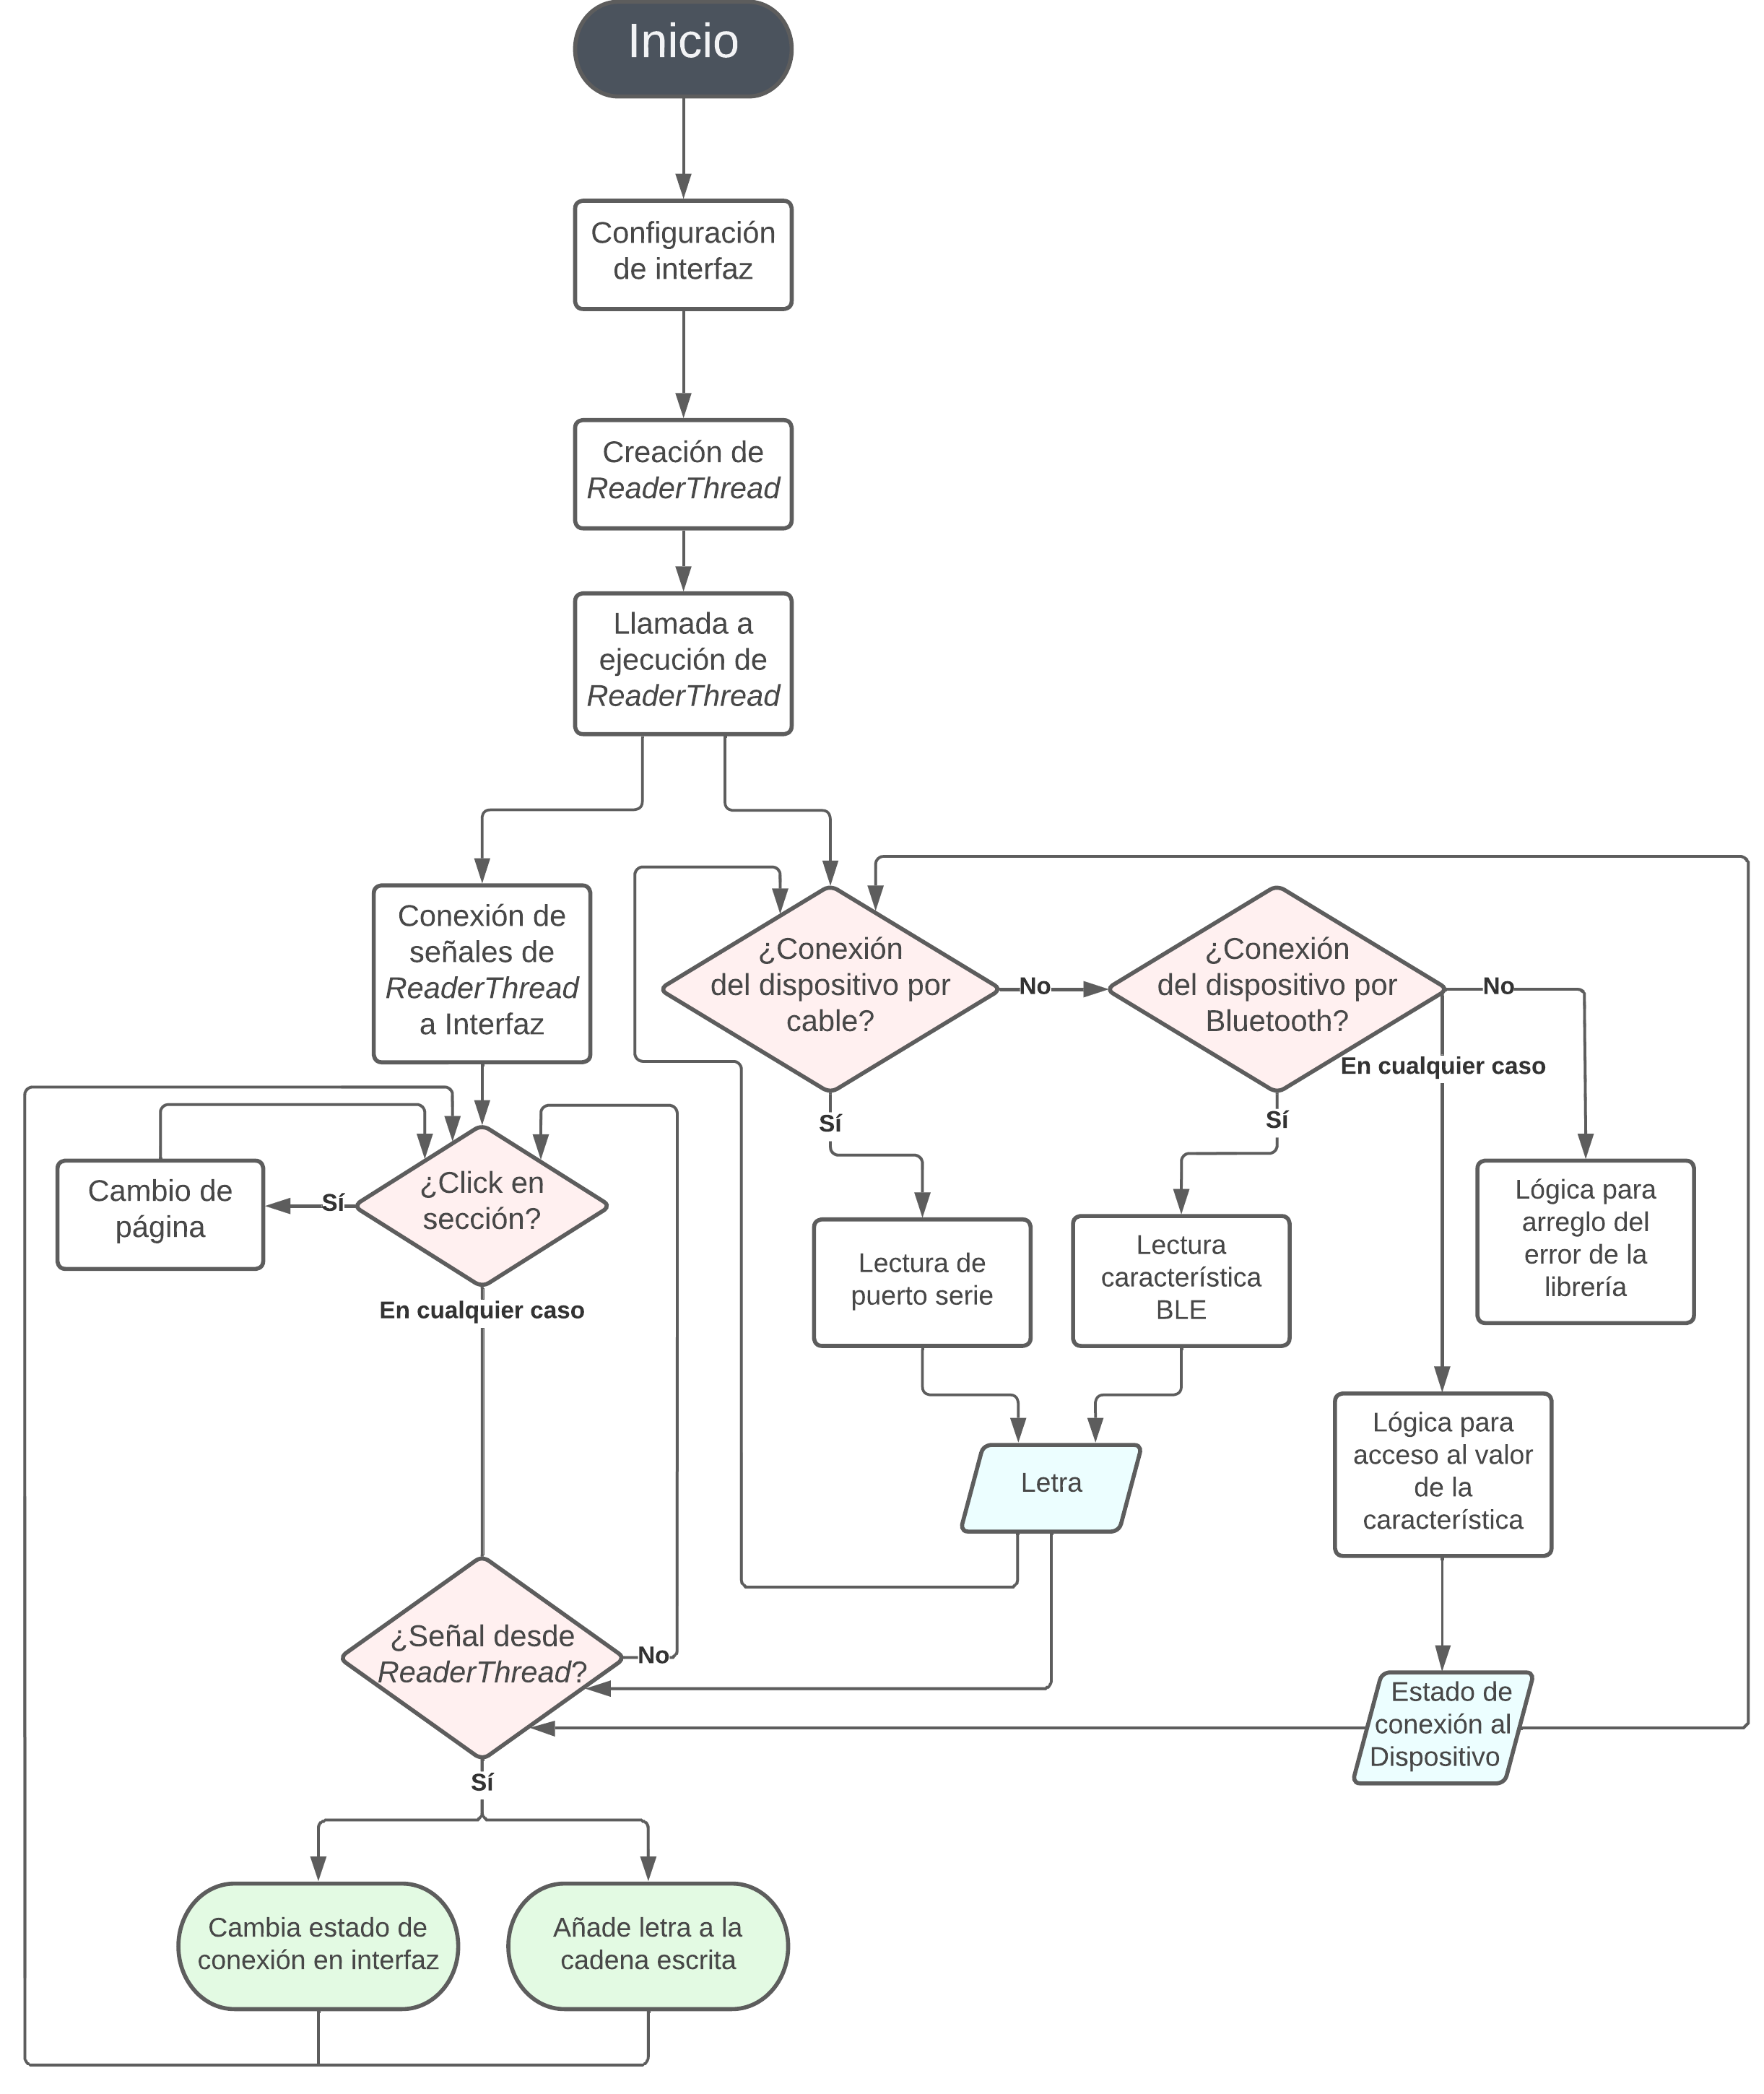
\includegraphics[width=1\textwidth]{capturas/DiagramaFlujoUI.png}\\[-0,20cm]
    \caption{Diagrama de flujo simplificado del \textit{UI}\label{diagFlujoQT}}
\end{figure}

\section{Configuración de la interfaz}
La configuración de la interfaz consistirá en inicializar los parámetros
con los que parten los elementos creados en la Sección \ref{trasaQT} anterior
y definir su comportamiento durante la ejecución.

Para el acceso a cada sección, se plantea un widget que varía su
contenido en función del índice seleccionado.
De esta forma se guarda el resto de la interfaz inmutable.
La configuración quedará de tal forma que al pulsar cada botón de sección,
cambiará título, sección seleccionada, y contenido de este widget.

Esta sección se basa de forma general, en fijación la trivial de parámetros
de estilo y establecer el comportamiento de los elementos dispuestos en pantalla.

\section{Gestión de lectura del microcontrolador}
El thread anteriormente citado en la Sección \ref{implemUI},
\href{https://github.com/AntonioPriego/SmartPen/blob/main/SmartPenUI/readerthread.cpp}{\textit{ReaderThread}}
será el encargado de esta labor, aunando en una única señal, las lecturas
de \textit{Bluetooth} y \textit{puerto serie}, y definiéndose de esta forma
como una interfaz de lectura para el programa. Esta interfaz de comunicación
entre 
\href{https://github.com/AntonioPriego/SmartPen/blob/main/SmartPenUI/readerthread.cpp}{\textit{ReaderThread}}
e interfaz se llevará a cabo mediante \textit{señales} y
\textit{slots}\textsuperscript{\cite{signalsQT}}
de \textit{QT}. Y será así porque es una forma de comunicación que permite
la interacción entre entidades concurrentes de una manera cómoda e intuitiva.


\subsection{Lectura de la característica \textit{Bluetooth Low Energy}}
Para esta sección será determinante una buena documentación, ya que la
implementación es un poco complicada cuando nunca se ha trabajado antes
con esta tecnología. Gracias a contar con ello como requisito para
la elección del \textit{framework} de creación de la \textit{UI},
podemos contar con documentación al respecto\textsuperscript{\cite{ejBLE}}.
Aunque es reseñable que bien por complejidad de la arquitectura \textit{BLE}
o bien porque la documentación es sucinta en exceso, el proceso de aprendizaje
para estas librerías, puede llegar a ser más lento de lo que cabría esperar.

Se creará una clase auxiliar
(\href{https://github.com/AntonioPriego/SmartPen/blob/main/SmartPenUI/device.cpp}{\textit{Device}})
que lidie con la gestión \textit{bluetooth} del programa: búsqueda de
dispositivos, conexión al \textit{SmartPen}, notificación de estados de conexión,
obtención de servicios, características, descriptores y valores,
y evidentemente lectura de las letras. La comunicación entre 
\href{https://github.com/AntonioPriego/SmartPen/blob/main/SmartPenUI/device.cpp}{\textit{Device}}
y el
\href{https://github.com/AntonioPriego/SmartPen/blob/main/SmartPenUI/readerthread.cpp}{\textit{ReaderThread}}
se llevará a cabo, al igual que entre
\href{https://github.com/AntonioPriego/SmartPen/blob/main/SmartPenUI/readerthread.cpp}{\textit{ReaderThread}}
e interfaz, mediante \textit{señales} y \textit{slots}\textsuperscript{\cite{signalsQT}}.

\begin{problemas}{Error de permisos para \textit{qt.bluetooth}}
    \color{mitexto}
    En ocasiones se experimentan crashes durante la ejecución,
    unido a un error derivado del uso de \textit{bluetooth} en los \textit{logs},
    lo que me llevó
    a investigar este problema para resolverlo. Llegando
    a que se debía a un error de permisos con el protocolo
    que gestiona el \textit{bluetooth} en \textit{Linux} (\textit{BlueZ}),
    y que más adelante seguirá causando problemas, pero en este caso, pudo
    resolverse como indica el Apéndice \ref{permBTQT}.
\end{problemas}

\begin{problemas}{Errores de desconexiones \textit{Bluetooth Low Energy}\label{errDescBT}}
    \color{mitexto}
    Posiblemente el error que más tiempo ha ocupado y que lamentablemente
    como desarrollador, solo se puede mitigar. Y es que es un problema
    aparentemente popular entre los desarrolladores que implementan 
    mecanismo \textit{bluetooth LE} para \textit{linux}, ya que se experimentan
    desconexiones del dispositivo sin aparente causa, ya que no son debidas
    a la implementación del desarrollador, sino de la librería que gestiona
    las comunicaciones \textit{bluetooth} en \textit{QT} haciendo uso de los
    protocolos provistos por \textit{linux}.

    Resulta especialmente problemático, no por el hecho de la desconexión,
    que también, sino porque se pierden valores durante esta; provocando
    sensación de que el dispositivo no funciona como debe. La pérdida de
    valores, tras mucha investigación y el aporte de la comunidad, tiene
    solución editando la propia librería que causa el problema;
    desarrollado en el apéndice \ref{errlibQTBT}.
    
    Desafortunadamente,
    el problema de las desconexiones persiste y aparenta deberse a
    \textit{BlueZ}, el \textit{stack} de \textit{bluetooth} de \textit{linux},
    que provee de los protocolos y capas necesarias para trabajar con este.
    Y por tanto, su solución queda fuera de mi margen de actuación, o al
    menos en un tiempo tan limitado. Sin embargo sí que he implementado un
    un ajuste para que de cara al usuario, solo suponga un pequeño retardo,
    en ocasiones, de la letra escrita y que se basa en el número de iteraciones
    en el proceso de conexión sin que se notifique señal por parte del
    dispositivo periférico; de forma que sí se notifique una desconexión
    persistente real, pero no las desconexiones provocadas por la falla
    descrita.
\end{problemas}

Pese a los problemas que se han encontrado, y que no podían sospecharse
hasta adentrarse en la implementación, el resultado es satisfactorio
y la experiencia de usuario es prácticamente la misma que si no
existieran estos problemas.


\subsection{Lectura del \textit{puerto serie}}
La implementación para la lectura del \textit{puerto serie} es mucho más sencilla
que la de \textit{bluetooth}. Como la gestión es mucho más simple
y apenas es necesario trabajar con una sola clase que media con el
\textit{puerto serie}, se implementará en una simple función de lectura
en el propio
\href{https://github.com/AntonioPriego/SmartPen/blob/main/SmartPenUI/readerthread.cpp}{\textit{ReaderThread}},
la cual se ejecutará en caso de que
se detecte conexión en el puerto serie y que será, el caso predeterminado
cuando exista posibilidad simultánea de conexión por cable e inalámbrica.

Véase el Apéndice \ref{psQT} para acceder a detalles de la implementación
para la lectura del puerto serie.

	% Entrenamiento
	%\begin{mimargen}{-0.65cm}{-1cm}
\chapter{Entrenamiento}

Para comenzar con Arduino+TensorFlow, instalaré la bibliotecas
necesarias para usar TensorFlow y la \textit{Nano 33 Sense}:
\begin{enumerate}
    \item \textbf{Arduino\_TensorFlowLite}: Permite construir aplicaciones con
    aplicaciones para AI/ML.
    \item \textbf{Arduino\_LSM9DS1}: Provee de las herramientas para acceder al
    acelerómetro, magnetometro y giroscopop del \textit{Nano 33 BLE Sense}.
\end{enumerate}

\cite{github-magicwand}Además, hay que realizar una serie de cambios en la biblioteca
\small\textbf{LSM9DS1.cpp}.\normalsize\\
Añadir justo antes de que la función \small\textbf{LSM9DS1Class::begin()}\normalsize
~retorne:
\begin{lstlisting}
    // Enable FIFO (see docs https://www.st.com/resource/en/datasheet/DM00103319.pdf)
    writeRegister(LSM9DS1_ADDRESS, 0x23, 0x02);
    // Set continuous mode
    writeRegister(LSM9DS1_ADDRESS, 0x2E, 0xC0);
\end{lstlisting}

También debemos editar \small\textbf{LSM9DS1Class::accelerationAvailable()}
\normalsize:
\begin{lstlisting}
    int LSM9DS1Class::accelerationAvailable()
    {
        /********************************** OLD *********************************
        if (readRegister(LSM9DS1_ADDRESS, LSM9DS1_STATUS_REG) & 0x01) { 
            return 1; 
        }
        *********************************** OLD *********************************/
    
        // Read FIFO_SRC. If any of the rightmost 8 bits have a value, there is data
        if (readRegister(LSM9DS1_ADDRESS, 0x2F) & 63) {
            return 1;
        }
        
        return 0;
    }
\end{lstlisting}

Si queremos acceder al puerto serie de la placa o usar el IDE de Arduino, debemos
conceder permisos al dispositivo:
\begin{lstlisting}[language=bash]
    ~$ ls -l /dev/ttyACM*                     # En mi caso
    ~$ sudo usermod -a -G dialout <usuario>
\end{lstlisting}~\\


Cuando ya tenemos la biblioteca para los sensores y el acceso al puerto garantizado,
podemos pasar a probar el programa.
Si funciona con el entrenamiento por defecto, continuamos finalmente con nuestro
entrenamiento.\\
Realizaremos el entrenamiento recogiendo muestras para cada caracter a
reconocer. Una vez tenemos suficientes muestras para todos los caracteres, podemos
realizar el entrenamiento del modelo, que realizaremos en \textit{Google Colab}.
El script de entrenamiento es el siguiente: [\textbf{METER ENLACE}].

~\\
Toma de muestras, para el software que utilizaremos para tomar los datos
para crear el dataset con el que entrenar el modelo, necesitaremos instalar las
siguientes bibliotecas:\\
\cite{apds9960} Arduino\_APDS9960: para disponer de librerías para algunos sensores adicionales.\\
\cite{cmsisdsp} Arduino\_CMSIS\-DSP: para disponer de arm\_math.h.\\
\cite{lps22hb} Arduino\_LPS22HB: herramientas para disponer del sensor de presión.\\
\cite{hts221} Arduino\_HTS221: herramientas para el sensor de temperatura y humedad.

\end{mimargen}

	% Notas
	%\input{capitulos/apendice.tex}

	% Notas
	%\begin{mimargen}{-1cm}{-1cm}

\chapter{Intento Harvard}

Comienzo ejecutando tal cual el código del repo
\url{https://github.com/petewarden/magic_wand}.

Importante tener la biblioteca de tensorflow actualizada(en este
caso la provista por pete warden).

Visto cómo toma pete los datos, pruebo a hacerlo.
Cargar el programa de recolección de datos en la placa(creo que funciona el magic\_wand,
PROBAR).
Acceder a la web de recolección. Recolectar.
Para acceder a la web, hay que hacerlo con chrome y con la flag
'Experimental Web Platform features' activa en 'chrome://flags/'


Hay un error con el DataCollector, además de que asigna mal los índices(index)
al borrar muestras, no guarda todas las muestras que tomas, da la sensación de que
hay un límite.
Para contar el número de muestras que hay en el JSON, uso la siguiente línea bash:
\begin{lstlisting}[language=bash]
~$ grep -o index <nombre_archivo>.json | wc -l
\end{lstlisting}



\textbf{CAMBIAR ORIENTACIÓN DE LA PLACA} \\
Como no hay referencias de la orientación original de los sensores en ningún
datasheet, con el propio sketch que hice originalmente para tomar las muestras,
comprobé la posición con la que funciona, la comparé con la posición que quiero
tener y gracias a eso pude hacer el siguiente cambio.\\
Lo mejor que he conseguido cambiando en la biblioteca de los sensores,
en LSM9DS1.cpp en todas los sensores:
\begin{lstlisting}[language=c++]
//          Original         //     Orientacion cambiada
x = data[0] * 4.0 / 32768.0; // z = -data[0] * 4.0 / 32768.0;
y = data[1] * 4.0 / 32768.0; // y =  data[1] * 4.0 / 32768.0;
z = data[2] * 4.0 / 32768.0; // x =  data[2] * 4.0 / 32768.0;
\end{lstlisting}

\newpage
Creo que habría que cambiar algo de deep\_pen.ino(a partir de línea 408)
\begin{lstlisting}[language=c++]
    const float gy = current_gravity[1];
    const float gz = current_gravity[2];
    float gmag = sqrtf((gy * gy) + (gz * gz));
    if (gmag < 0.0001f) {
      gmag = 0.0001f;
    }
    // ...
\end{lstlisting}


\textbf{LA OBTENCIÓN DE DATOS TIENE UN FALLO AL BORRAR MUESTRAS} \\
Este fallo aparentemente se produce al borrar instancias por debajo de
la última. En ocasiones, se produce un pequeño error en las comprobaciones
de índices de muestras, por lo que se borran varias muestras y estas terminan
con índices desordenados.\\
Para paliar este problema, he creado un pequeño script que toma el número de
muestras y ordena los índices de las mismas.\\

\textbf{MODELO}\\
Se trata de un modelo de aprendizaje supervisado, es decir, que está basado en
etiquetas(\textit{labels}) estas etiquetas representarán las distintas soluciones
a las que hará frente el modelo; en nuestro caso, letras.
La forma que emplearemos para representar dichas letras como input para el modelo,
serán imágenes. Aunque para tomar dichas imágenes, hacemos uso del giroscopio
y el acelerómetro de la placa.\\


\textbf{LEER DEL PUERTO SERIE EN QT}
Hay que añadir al *.pro del proyecto QT:
\begin{lstlisting}[language=make]
  QT += serialport
\end{lstlisting}
Y tras esto, añadir la biblioteca con normalidad y acceder al puerto
con el nombre, en nuestro caso, "ttyACM0".\\\\

\textbf{FALLO RECONOCIMIENTO DE IMÁGENES QT}\\
Al importar imágenes en QT tras haber exportado el programa a Win y Linux para
probar que todo fuera correctamente, las imágenes dejaron de mostrarse.\\
Esto se debe a que cambió la ruta del proyecto al directorio en el que se
exportó. Por tanto las rutas especificadas para las imágenes, dejaron de ser
válidas. Para corregir este problema, basta con cambiar el 'Build directory' del
proyecto(Desde 'Projects' en el panel de la derecha del QT creator).\\

\textbf{HEBRAS QT}\\
Para la lectura del puerto serie desde el programa, necesitamos imporat

\textbf{VISOR WEB QT}\\
Para hacer empotrar html en qt, importamos las bibliotecas de QWeb. Para ello,
necesitamos aantes instlar todo el QtWebKit siguiendo las instrucciones:
\url{https://github.com/OpenBoard-org/OpenBoard/wiki/Build-OpenBoard-on-Ubuntu-20.04}

\textbf{VINCULAR PUERTO SERIE A PLACA}\\
Para ello, haré uso de las reglas de udev del sistema linux.
Lo primero es conocer la información de nuestra placa:
\begin{lstlisting}[language=make]
  ~$ lsusb
[...]
Bus 003 Device 004: ID 2341:805a Arduino SA Nano 33 BLE
[...]
\end{lstlisting}
De aquí podemos extraer el fabricante(o idVendor) y el producto de este fabricante
(o idProduct). Necesitaremos ambos.

Ahora necesitamos el serial del puerto al que vincularemos la placa:
\begin{lstlisting}[language=make]
  ~$ udevadm info -a -n /dev/ttyACM0 | grep serial
ATTRS{serial}=="185F25FD3EF48040"
\end{lstlisting}
Con esto, ya podemos crear la regla para vincular univocamente el puerto a la placa
y evitar así problemas con la detección en el UI.\\
En /etc/udev/rules.d/99-ftdi.rules (en mi caso, varía dependiendo del sistema),
crearemos la regla \\SUBSYSTEM=="tty", ATTRS{idVendor}=="2341", ATTRS{idProduct}=="805a",
ATTRS{serial}=="185F25FD3EF48040", SYMLINK+="ttySLAB0"\\por los datos obtenidos.\\

\textbf{CAMBIOS MODELO}\\
Cambiar el tamaño del kernel de las capas Conv2D de 3 a 4, resulta muy efectivo,
a costa, evidentemente, de aumentar el tamaño que ocupa el modelo.\\
Al pasar de 4 a 5, el modelo arroja unos datos de efectividad teóricos extremadamente
buenos, alcanzando cifras de precisión mucho más altas con menos epochs.
En general, podemos extrapolar que, a mayor tamaño del kernel, mejor precisión pero
mayor tamaño del modelo. En nuestro caso no llega a ser un problema, ya que, aunque
estamos usando un dispositivo de memoria limitada, no llega a ocuparse toda la memoria
del mismo, al menos por ahora.\\

\textbf{PRUEBAS BLUETOOTH}\\
He tenido que instalar qtconnectivity5-dev para probar el QT project que estoy probando.\\

\textbf{POR QUÉ ESTA PLACA?}\\
Aduino Nano Sense 33 BLE\\
Por qué arduino: Documentación, respaldo comunidad, IDE facilita trabajo, etc.\\
Por qué Nano: Queremos integrarla en un 'lápiz', debe ser un dispositivo pequeño.\\
Por qué Sense: Necesitamos los sensores para el reconocimiento de movimiento.\\
BLE: Por pura utilidad, es mucho más cómodo utilizar el lápiz de forma inalámbrica.
Además no tiene mucho sentido integrar el procesamiento en un dispositivo pequeño
si va a depender de un ordenador.\\

\textbf{DESCONEXIÓN DEL PROGRAMA A BT AL ESCRIBIR PLACA EN RX}\\
Para el control de flujo de la comunicación bluetooth(asegurarse de que recibimos
bien y solo una vez cada letra), implemento un sistema de señales.
Cuando recibimos una letra desde la placa(mediante canal tx), el programa la almacena y
envía una señal de que ha recibido la letra(mediante canal rx) y cuando la placa
recibe esta señal, borra del canal tx la letra para que no vuelva a leerse desde el
programa.
El problema descrito, viene, creo, al escribir en rx la señal de recibo. Por algún
motivo, el programa se desconecta de la placa.\\


\textbf{MÉTODO DE ENVÍO DE BUFFER DE LETRAS PARA CONEXIÓN BT CUANDO HAYA UNA CADENA
PREVIA A CONEXIÓN}\\

~\\~\\~\\Documentación Bluetooth LE:
https://doc.qt.io/qt-6/qtbluetooth-le-overview.html

~\\~\\~\\Visualizar red neuronal :
http://alexlenail.me/NN-SVG/index.html

~\\~\\~\\Documentación sobre Keras:
https://keras.io/api/

\end{mimargen}

	% Desarrollo bajo sprints: 
	% 	1. Permitir registros y login de usuarios
	% 	2. Desarrollo del sistema de incidencias
	% 	3. Desarrollo del sistema de denuncias administrativas y accidentes
	% 	4. Desarrollo del sistema de croquis
	%   5. Instalación de la aplicación de manera automática
	%\chapter{Implementación}

La implementación del software se ha dividido en hitos. Estos, han sido definidos en Github
y cada uno de ellos contiene un grupo de \textit{issues} que se corresponden con las distintas
mejoras que se han ido incorporando al software a lo largo de su desarrollo.\\



	% Encapsulado
	\chapter{Encapsulado\label{encapsulado}}
Para esta parte, dada la menor relevancia al poner en contexto todo el proyecto, se
contará con poco tiempo. Esto supondrá decisiones tomadas con esta limitación,
\section{Herramientas utilizadas}
Para la creación de los modelos 3D del encapsulado, se han utilizado principalmente
dos herramientas distintas para modelar y una para imprimir.

Para el modelado se utilizará \textit{Blender}, un software de modelado muy potente
y lleno de posibilidades, aunque considerablemente complejo al empezar y que utilicé
para no limitar el modelo a algo simple. Fuera de lo
planificado, también se ha utilizado \textit{SketchUp}.

Para la impresión, de la que yo no me encargaré, se hará uso del \textit{slicer}
(software para impresión 3D) \textit{Ultimaker Cura}.

\section{Implementación}
Por la limitación de tiempo descrita al comienzo de este capítulo \ref{encapsulado},
no se dispone de tiempo para una fase de diseño previa a implementar el modelo.
El modelo se ha construirá con las especificaciones más básicas en mente.

El encapsulado debe contener de forma firme el microcontrolador para que no se mueva,
ya que se espera que el usario lo mueva con determinación para trazar una letra. Por
otro lado, también será necesario incorporar una batería para alimentarm sin conexión
directa al ordenador, el dispositivo. Con estas dos únicas limitaciones y con una forma
semejante a la de un bolígrafo, se construirá el modelo.

El modelo estará dividido en partes por motivos de la logística de la impresión, tanto
por comodidad para tratar con la persona que lo imprimirá, como por cuestiones de que los
modelos deben guardar ciertas limitaciones estructurales para poder imprimirse. Por ejemplo,
en lugar de imprimir el
\href{https://github.com/AntonioPriego/SmartPen/tree/main/SmartPenModel/Components/cilindroBajo}{cilindroBajo}
ya con la 
\href{https://github.com/AntonioPriego/SmartPen/tree/main/SmartPenModel/Components/punta}{punta},
para aunar toda la parte inferior del encapsulado, se imprimen por separado ya que se necesita de
una base estable para la impresión que no se lograría con los dos elementos unidos.

\begin{problemas}{Modelo incompatible con la impresión}
    \color{mitexto}
    Durante la impresión la impresión surgieron varios problemas, la mayoría menores,
    sin embargo hubo uno se resistió aunque no entrañaba realmente ninguna complejidad.
    Este era que una de las partes del encapsulado, el
    \href{https://github.com/AntonioPriego/SmartPen/tree/main/SmartPenModel/Components/cilindroBajo}{cilindroBajo},
    la parte en contendrá el microcontrolador, mostraba en el \textit{slicer} (software
    para la impresión), un error de formato en la base. Este error finalmente se debía
    a un grosor por debajo del mínimo. Problema ocasionado por haber construido
    a partir del escalado vertical de otro componente
    (\href{https://github.com/AntonioPriego/SmartPen/tree/main/SmartPenModel/Components/cilindroAlto}{cilindroAlto});
    al escalar verticalmente, el grosor de la pared del modelo, se conserva, sin embargo
    no ocurre lo mismo para la base, disminuyendo su grosor y provocando este problema.
    La solución fue simplemente redefinir el grosor de la base.
\end{problemas}

Con todos los componentes impresos, surge un problema con la batería con la que contaba
para incorporar en el encapsulado

\begin{problemas}{Alimentación intermitente de la batería}
    \color{mitexto}
    La alimentación resultaba deficiente, por lo tanto solo pude hacerme con
    otra batería y adaptar el encapsulado a este nuevo componente.
    Para poder crear el modelo complementario para adaptar la batería, hice uso
    de \textit{SketchUp}, un software muchísimo más simple que \textit{Blender};
    esta sencillez ha sido determinante porque el tiempo era muy restrictivo en ese momento.
    Resultando en el componente
    \href{https://github.com/AntonioPriego/SmartPen/tree/main/SmartPenModel/Components/slotBateria}{slotBatería},
    para poder incluir una pila de 9V recargable. La alimentación con esta pila, al ser de más
    de 5V, deberá ser vía pines de la placa, que admiten hasta 21V.
\end{problemas}

Con esta nueva batería, se logra una autonomía de más de dos días en el primer ciclo
de carga. Según el fabricante, los primeros ciclos de carga suelen ser los que menor
energía suministran, por lo que podría incluso mejorar la duración.

En los Apéndices \ref{modelos} y \ref{encapsulado} pueden encontrarse ilustrados,
respectivamente, los modelos creados y el resultado final del encapsulado con
todo el hardware integrado.

	% Validación
	\chapter{Validación}

\section{Ajuste al presupuesto}
Respecto a como se estimó en la sección \ref{presupuesto} (\textit{Presupuesto}),
se ha ajustado satisfactoriamente el coste del dispositivo, resultando todos los costes
los reflejados en la Tabla \ref{tabPresFin}.
\begin{table}[h]
    \begin{tabular}{ll}
    \hline
    \rowcolor[HTML]{6665CD} 
    \multicolumn{1}{|l|}{\cellcolor[HTML]{6665CD}{\color[HTML]{EFEFEF} \textbf{Descripción}}} & \multicolumn{1}{l|}{\cellcolor[HTML]{6665CD}{\color[HTML]{EFEFEF} \textbf{Precio}}} \\ \hline
    \multicolumn{1}{|l|}{Arduino Nano Sense 33 BLE ~~~~~~~~~~~~~~~~~~~~~~~~~~~~~~~~~~~~~}& \multicolumn{1}{r|}{35'80\$$\sim$33'82€}                                            \\
    \multicolumn{1}{|l|}{Pila 9V Recargable}                                                  & \multicolumn{1}{r|}{10'99€}                                                         \\
    \multicolumn{1}{|l|}{Adaptador pila 9V}                                                           & \multicolumn{1}{r|}{3€}                                                             \\
    \multicolumn{1}{|l|}{Impresión}                                                           & \multicolumn{1}{r|}{1€}                                                             \\
    \multicolumn{1}{|l|}{Interruptor}                                                           & \multicolumn{1}{r|}{0'05€}                                                             \\
    \multicolumn{1}{|l|}{Adaptador microUSB a USB}                                                           & \multicolumn{1}{r|}{1€}                                                             \\
    \multicolumn{1}{|l|}{Cable MicroUSB Datos}                                                & \multicolumn{1}{r|}{6€}                                                             \\ \hline
    \multicolumn{1}{r}{\textbf{TOTAL:}}                                                       & \textbf{55,86€}                                                                    
    \end{tabular}
    \caption{Costes de producción del \textit{SmartPen}\label{tabPresFin}}
\end{table}

Respecto a las horas de trabajo, también se ha respetado la estimación de
la planificación, ya que he tratado de ceñirme a estas durante todo el desarrollo del
proyecto.

\section{Comprobación de objetivos cumplidos}
Los requisitos para el proyecto y sus derivadas especificaciones, han sido
satisfactoriamente cumplidas.

El presupuesto se ha ajustado a lo estimado tanto en su aspecto de trabajo
como en el de ajuste para los fondos empleados en el \textit{hardware}.

El microcontrolador efectivamente, como se propuso, hace uso de un modelo
basado en \textit{Deep Learning} y además lo hace de manera eficaz. Para
alimentar al modelo de procesamiento se hace uso de los sensores que ofrece
el microcontrolador, el cual cuenta con dimensiones muy reducidas para
poder acoplarse en un encapsulado embellecedor que dará cabida también
a una batería que lo alimentará para, como se especifica, dotarlo de autonomía.
Autonomía necesaria ya que el dispositivo funciona tanto por cable
como de forma inalámbrica, tal y como se demandaba.

Todo el desarrollo es transparente y de código abierto, por lo que
está acondicionado para que otros desarrolladores y usuarios hagan uso del progreso logrado
en este despliegue del producto y aporten funcionalidades al producto
si así lo consideran.

Todo el \textit{software} utilizado cumple con las especificaciones, porque de otra forma,
no podría haberse llevado a cabo el proyecto.
La interfaz de usuario cumple con la funcionalidad mínima propuesta;
el \textit{framework} para el diseño, entrenamiento, validación y testeo
de la \textit{red neuronal} es el mejor que podría haberse empleado;
el \textit{firmware} del microcontrolador ejecuta exactamente lo que
se ideó al comienzo del proyecto; y respecto al \textit{software} para 
el modelado del encapsulado, se han trabajado con varias alternativas
en función de lo que se requería en cada momento.

En general el producto no solo realiza su cometido, sino que lo hace
de forma satisfactoria.
{\color{red} Añadir 'como muestra tal' si da tiempo a demo}

	% Trabajos futuros
	\chapter{Trabajos futuros y mejoras}
Si bien el dispositivo realiza lo que se postulaba al comienzo
como requerimientos. Sin embargo quedan muchas mejoras y ampliaciones
posibles, en su mayoría por carencia de tiempo.

Una de las que más me incordian, es el no haber podido añadir
la funcionalidad de 'modo pizarra', ya que si bien no estaba planteado
como requisito, era algo que pretendía hacer desde el planteamiento del
trabajo, ya que me resulta especialmente útil como complemento a una
herramienta que pretende ser un híbrido entre lápiz y teclado.
De hecho la solución era integrar el módulo de exposición del trazado
de la herramienta de recolección de datos
(\href{https://github.com/AntonioPriego/SmartPen/blob/main/DataCollector/SmartPen_DataCollector.html}{\textit{SmartPen\_DataCollector}})
en el propio interfaz de usuario, haciendo uso de las herramientas de \textit{QT}
para visualización web. Sin embargo al emplear la web \textit{bluetooth}
para la recolección del trazo generado por el microcontrolador, dificultaba
mucho la implementación y viendo que se alargaría más de lo esperado,
se tomó la decisión de postergarlo.

Otro añadido que habría dado más autonomía al dispositivo, es el uso
de un buffer de memoria en el microcontrolador para almacenar
las letras que se escribieran previas a la conexión con la interfaz
de usuario. Y que es en realidad una funcionalidad muy fácil de implementar
ya que solo habría que crear el propio buffer en el microcontrolador
y cambiar la lógica de la comunicación interfaz-microcontrolador de una
letra a varias letras consecutivamente enviadas.

Esta sin embargo sería una mejora mucho más compleja y que llevaría
un proceso de documentación a bajo nivel, un tanto distendido.
El problema de desconexiones descrito en Problemas \ref{errDescBT}.
La solución sería encontrar el problema que desemboca en la desconexión
y que parte de la librería mencionada y el stack de protocolos \textit{bluetooth}
de \textit{linux}.

Lo cual nos lleva a otra posible mejora y es la implementación de la interfaz
para \textit{Windows} o \textit{macOS}. Me gustaría poder haberla realizado, pero el tiempo
no alcanza para más y dado que trabajo habitualmente en \textit{linux},
era más inteligente comenzar implementando la interfaz solo para este sistema.
En principio la solución pasaría por, simplemente, añadir la configuración de
puertos correspondientes para cada sistema.

Una mejora que significaría un rango mucho mayor de detección para el \textit{SmartPen}
y algo más de precisión, sería aumentar el número de muestras con el que
entrenar el modelo. Pero como se expuso en la Sección \ref{dataColl}, es un proceso
que lleva muchísimo tiempo. Aunque sencilla, esta mejora supone emplear tiempo
del que no se dispone.

En realidad hay un sinfín de posibles mejoras y nuevas funcionalidades,
pero por esto mismo y dado que es un proyecto interesante y lleno de
posibilidades, se ha planteado su desarrollo abierto y libre a aportaciones de
la comunidad.

	% Conclusiones
	\chapter{Conclusiones}
Las conclusiones tras el desarrollo del proyecto y ver los resultados, son que
es algo de lo que estaría orgulloso si lo hubiese visto al comienzo del mismo.
Sin embargo no puedo evitar sentir que, por todo lo que tenía en mente
haber implementado, podría haber sido incluso mejor. Aunque ya pude suponer
desde el principio que el tiempo del que disponía no era suficiente para llenar
de funcionalidades el proyecto, por eso planteé lo que queda descrito en esta
memoria de la forma que lo hice y he cumplido con ello de forma satisfactoria.

Por otro lado, el haber trabajado con \textit{Deep Learning}, \textit{redes neuronales},
\textit{capas}, \textit{entrenamientos} y otros tantos conceptos que me resultaban tan llamativos
e interesantes, y haberlo podido unir al campo del \textit{hardware} que tanto
me apasiona, mediante la integración del procesamiento en un microcontrolador,
es otra de las razones por las que me complace haberme decidido por este proyecto.

Ha sido un trabajo complicado desde su propio planteamiento, los complejos mecanismos
que se emplean, el no haberlos utilizado nunca antes y por los problemas
que han ido surgiendo durante el desarrollo, fruto de la implementación.
Pero el resultado y el aprendizaje surgido del esfuerzo para poder completarlo,
han hecho que valga la pena.

Finalmente, es necesario concluir que este no es el final de este proyecto,
planeo continuar con su desarrollo como pasatiempo y me llenaría de orgullo
que otras personas interesadas en estos campos, participaran también
agregando sus aportaciones como se plantea al hacer todo el proyecto
público y abierto.
\newline\newline
\url{https://github.com/AntonioPriego/SmartPen}

	\newpage
	\nocite{*}
	%{\raggedright
	\bibliography{bibliografia}
	\bibliographystyle{plain}

	% Apéndice
	\appendixpageoff % Eliminar la página introductoria a apéndices

\begin{appendices}
\chapter{Microcontrolador}
\section{Resolver problemas de memoria\label{memFlash}}
A lo largo del desarrollo del firmware, será necesaria la gestión de
áreas de memoria reservadas para ciertas funcionalidades, por ejemplo
en el bloque de configuración del firmware, \textit{setup()}; será
necesario reservar un área en memoria para las labores de E/S y memoria
intermedia de las acciones con tensor.

Para ello se contará con la propia \textit{flash}
del dispositivo a modo de región de almacenamiento. Creando arrays en la
propia memoria \textit{flash} que harán las veces de mecanismo de
almacenamiento como se expone en el siguiente fragmento de código:\\

\begin{lstlisting}[firstnumber=62,title=Fragmento de \textit{deep\_pen.ino}]
    /************************ SETUP FUNCTION ************************/
    // Setting the area of memory reserved to tensor input-output actions.
    constexpr int TensorAreaSize = 30 * 1024;
    uint8_t tensor_arena[TensorAreaSize];
\end{lstlisting}


\section{Instalación de librerías en \textit{Arduino IDE}\label{libArduino}}
La instalación de librerias es muy sencilla haciendo uso del
\textit{Arduino IDE}. En el menú: \textit{Tools}->\textit{Manage
Libraries...} y se abrirá una ventana donde podemos gestionar las
librerías instaladas, instalar otras versiones e instalar nuevas
librerías.


\section{Notificación de conexión \textit{Bluetooth} del firmware
del microcontrolador\label{BTcon}}
Para solucionar el problema de la notificación de conexión \textit{Bluetooth}
se crea una pequeña estructura para consultar el estado de conexión de la iteración
anterior (\textit{last\_connection}). De esta forma es posible mantener consistencia
en la conexión pese a estar dentro de un bucle.


\section{Definición de micro-operaciones en el firmware del
microcontrolador\label{firmwMO}}
Las micro-operaciones que se definirán en el firmware que
se emplearán en la red neuronal son:
\begin{itemize}
    \itemsep0em 
    \item Conv2: Para el procesamiento de la capa homónima.
    \item Mean: Para promedios como el que se necesita en la capa \textit{GlobalAveragePooling2D}
    \item FullyConnected: Para las capas densas, entre otros.
    \item SoftMax: Como función de activación.
\end{itemize}

Como alternativa más cómoda, pero a costa de un mayor uso de memoria,
del cual no podemos abusar dada la naturaleza de nuestro dispositivo;
es plausible usar \textit{tflite::AllOpsResolver}, que cargará todas las
operaciones disponibles para \textit{TFLite}.


\section{Cambiar la orientación de la placa}
Para poder hacer uso del \textit{SmartPen} en una posición de escritura natural,
vertica, hay que hacer una serie de cambios.
Los mejores resultados se han conseguido cambiando en la biblioteca de los sensores,
en LSM9DS1.cpp en todas los sensores:
\begin{lstlisting}[firstnumber=121,language=c++,title=Fragmento
    de \textit{LSM9DS1.cpp} de la librería homónima]
//          Original         //     Orientacion cambiada
x = data[0] * 4.0 / 32768.0; // z = -data[0] * 4.0 / 32768.0;
y = data[1] * 4.0 / 32768.0; // y =  data[1] * 4.0 / 32768.0;
z = data[2] * 4.0 / 32768.0; // x =  data[2] * 4.0 / 32768.0;
\end{lstlisting}

Aunque continúan sin obtenerse trazados correctos del movimiento.


\chapter{Red neuronal}
\section{Ajuste para poder utilizar el recolector de muestras de
\textit{Pete Warden}\textsuperscript{\cite{petewardenmw}}\label{PWchrome}}
Es necesario hacer uso del recolector de muestras, utilizar \textit{Google Chrome}
y activar la flag para desarrolladores '\textit{Experimental Web Platform features}'
activa en '\textit{chrome://flags/}'.


\section{Asignación incorrecta de índices en el recolector de muestras\label{borraIndices}}
Como se ha citado en el \textit{apéndice \ref{borrarMuestras}} anterior,
al borrar muestras se borran más trazos de los debidos y eso genera
una redistribución de los índices de cada muestra, resultando incorrectos.

Para resolverlo, se ha creado un script que reasigna los índices con
la distribución adecuada: 
\href{https://github.com/AntonioPriego/SmartPen/blob/main/Utils/sort_dataset.py}{sort\_dataset.py}


\section{El recolector de muestras elimina varias muestras al borrar una\label{borrarMuestras}}
Este fallo aparentemente se produce al borrar instancias por debajo de
la última. En ocasiones, se produce un pequeño error en las comprobaciones
de índices de muestras, por lo que se borran varias muestras y estas terminan
con índices desordenados.

Para paliar este problema y comprobar si había el número de trazos esperado,
se hacía uso de un comando en bash cada vez que se generara un \textit{JSON}:

\begin{lstlisting}[language=bash]
    ~$ grep -o index <nombre_archivo>.json | wc -l
\end{lstlisting}


\section{Descripción de capas \textit{Keras} empleadas para la implementación
de la red neuronal\label{capasKeras}}

Las capas utilizadas durante la implementación del modelo,
son las siguientes\textsuperscript{\cite{keras}}:
\begin{itemize}
    \itemsep0em 
    \item Rescaling: Como resultado de esta capa,
    se consigue reescalar o normalizar
    los valores de los inputs, en nuestro caso las imágenes. Con esto definimos
    una escala uniforme y es un procedimiento típico en procesamiento de imagen:
    \textit{image normalization}, donde se normalizará el valor de los píxeles
    de las imágenes a una escala [0,1].
    \item Conv2D: Capa para procesamiento convolucional,
    es la capa que realmente
    procesará dentro del modelo. Se crea un kernel que convoluciona con la entrada
    de la capa. Se define la capa en base ciertos parámetros que determinarán su
    funcionamiento y complejidad, siendo en nuestro caso los parámetros:
    \begin{itemize}
        \itemsep0em 
        \item filters: el número de filtros de salida de la convolución.
        \item kernel\_size: el tamaño de ventana de convolución, cuando se
        especifica un solo número, se interpreta una ventana cuadrada de ese
        tamaño.
        \item strides: define el tamaño de los tramos de salto de la ventana
        de convolución.
        \item input\_shape: establecer el tamaño de la entrada. En nuestro caso
        imágenes de 32x32.
    \end{itemize}
    \item BatchNormalization: Normaliza sus entradas por lotes.
    Aplica transformaciones
    que conservan la media de la salida cercana a 0 y la desviación estándar a 1.
    \item Activation: aplica una función de activación a una salida. Las funciones de
    activación son las que arbitran la activación de las neuronas de la red neuronal
    y por ello, repercute en su salida. Existen diversas
    funciones de activación, como lo son \textit{rectified linear unit(relu)},
    \textit{sigmoid}, \textit{softmax}(función de distribución de probabilidad), etc.
    \item Dropout: Capa que introduce cierta entropía, de forma que se descarta
    la contribución de ciertas neuronas de forma estadística. Se suelen implementar
    para soslayar el \textit{overfitting}.
    \item GlobalAveragePooling2D: Esta capa tomará un
    tensor de dimensión $x*y*z$ y
    calculando el valor medio de los valores $x$ e $y$, producirá una salida basada en
    $z$ elementos.
    \item Dense: Es una capa común de red neuronal,
    solo que está \textit{densamente}
    conectada, es decir, cada neurona de esta capa está conectada a todas las neuronas
    de la capa anterior. Se usa, como es nuestro caso, en redes clasificatorias.
\end{itemize}

\begin{figure}[]
    \centering
    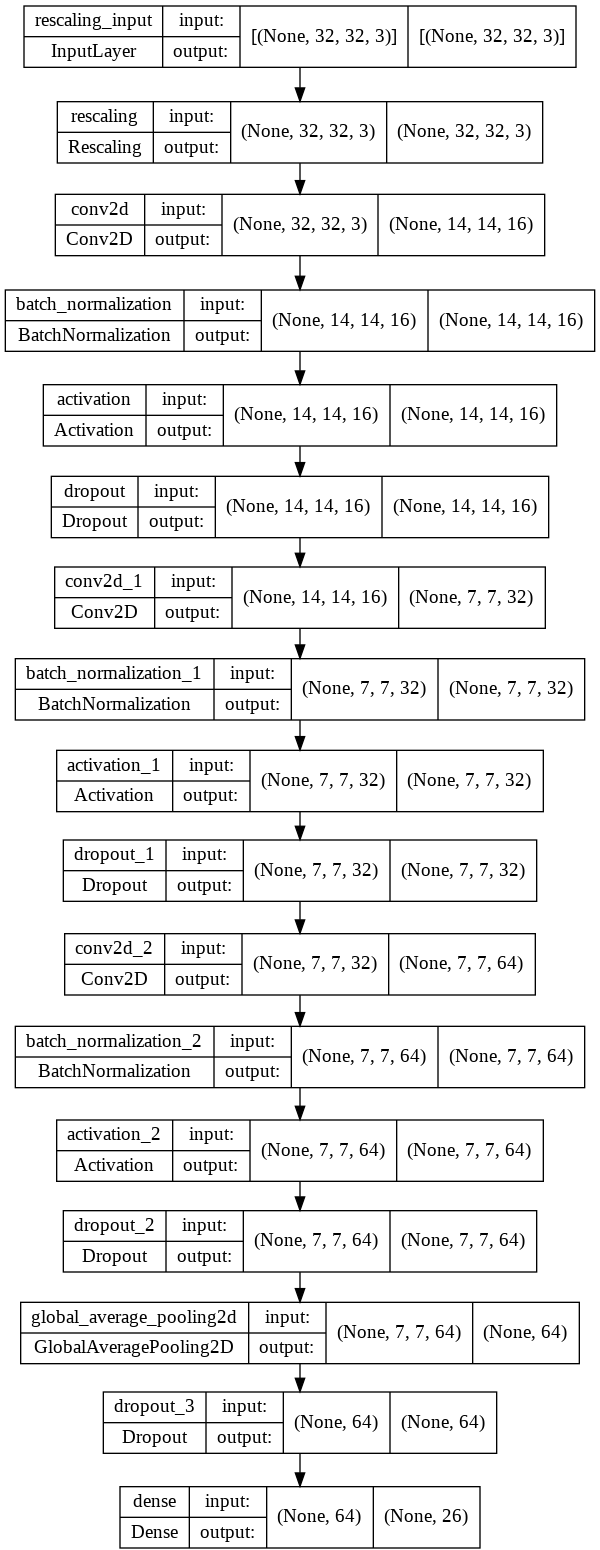
\includegraphics[width=0.7\textwidth]{capturas/estructuraRNTF.png}\\[-0,35cm]
    \caption{Estructura del modelo generado en \textit{TensorFlow}\label{estRN}}
\end{figure}

La anterior \textit{figura \ref{estRN}} es consecuencia del siguiente código:
\begin{lstlisting}[language=python, title=Fragmento de \textit{Train.ipynb}]
    ############## MAKING THE MODEL ###############

    def make_model(input_shape, num_classes):
      model = models.Sequential()
    
      # Rescaling
      model.add( layers.Rescaling(1.0 / 255) )
      # Block 1
      model.add( layers.Conv2D(16, 5, strides=2, input_shape=input_shape) )
      model.add( layers.BatchNormalization() )
      model.add( layers.Activation("relu") )
      model.add( layers.Dropout(0.5) )
      # Block 2
      model.add( layers.Conv2D(32, 5, strides=2, padding="same") )
      model.add( layers.BatchNormalization() )
      model.add( layers.Activation("relu") )
      model.add( layers.Dropout(0.5) )
      # Block 3
      model.add( layers.Conv2D(64, 3, strides=1, padding="same") )
      model.add( layers.BatchNormalization() )
      model.add( layers.Activation("relu") )
      model.add( layers.Dropout(0.5) )
      # Pooling + another Dropout
      model.add( layers.GlobalAveragePooling2D() )
      model.add( layers.Dropout(0.5) )
      # Softmax
      model.add( layers.Dense(num_classes, activation="softmax") )
    
    
      return model
    
    model = make_model(input_shape=(IMAGE_WIDTH, IMAGE_HEIGHT, 3),
                          num_classes=26)
    model.build(input_shape=(None, IMAGE_WIDTH, IMAGE_HEIGHT, 3))
    model.summary()
    keras.utils.plot_model(model, show_shapes=True)
\end{lstlisting}

\section{Experimentación red neuronal}
\subsection{Diseño de la red neuronal\label{expRN}}
{\color{red} Hablar sobre los cambios probados en la red neuronal y
sus resultados. Carpeta Train->Análisis\\\\
Cambiar el tamaño del kernel de las capas Conv2D de 3 a 4, resulta muy efectivo,
a costa, evidentemente, de aumentar el tamaño que ocupa el modelo.\\
Al pasar de 4 a 5, el modelo arroja unos datos de efectividad teóricos extremadamente
buenos, alcanzando cifras de precisión mucho más altas con menos epochs.
En general, podemos extrapolar que, a mayor tamaño del kernel, mejor precisión pero
mayor tamaño del modelo. En nuestro caso no llega a ser un problema, ya que, aunque
estamos usando un dispositivo de memoria limitada, no llega a ocuparse toda la memoria
del mismo, al menos por ahora.}

Cada uno de los modelos o cambios con los que se ha experimentado, son
pequeñas iteraciones o pequeñas variaciones respecto del modelo base.
Creado a partir del estudio de otros modelos para tareas parecidas.

Una de las abundantes variables con las que experimentar, es el
tamaño de las imágenes de entrada para la red neuronal. Se ha
percibido una notoria mejora en el reconocimiento con letras
complejas, como por ejemplo la 'k', a medida que las dimensiones aumentan. 
De forma análoga, con letras simples, como por ejemplo la 'c', a razón de
una menor resolución, mejores resultados se obtenían. Esto cuadra con lo
esperable, ya que las letras complejas necesitan de un análisis más preciso
para obtener mejores predicciones que el resto y equivalentemente, las letras
más sencillas obtienen mejores predicciones sobre el resto, cuando se analizan
muestras sencillas.

\subsection{Entrenamiento de la red neuronal\label{expTrainRN}}
{\color{red} ENTRENAMIENTO: Hablar de \textit{epochs}, \textit{learning\_rate},
\textit{optimizadores}, etc.}
{\color{red} ENTRENAMIENTO: Resultados del testeo obtenidos de los modelos
Carpeta Train->Análisis.}


\chapter{Interfaz de usuario}
\section{Permisos uso del puerto del microcontrolador (Linux)\label{pserie}}
En algunos casos, como ocurrió en el trascurso de este trabajo,
si queremos acceder al puerto serie de la placa o usar el IDE de
Arduino, debemos conceder permisos al microcontrolador:
\begin{lstlisting}[language=bash]
    ~$ ls -l /dev/ttyACM*                     # En mi caso
    ~$ sudo usermod -a -G dialout <usuario>
\end{lstlisting}

Como respuesta al error ``\textit{can't open device /dev/ttyACM0}''.


\section{Acceso al puerto serie en QT (Linux)\label{psQT}}
Hay que añadir al *.pro del proyecto QT:
\begin{lstlisting}[language=make]
  QT += serialport
\end{lstlisting}
Y tras esto, añadir la librería con normalidad y acceder al puerto
con el nombre, en nuestro caso, "ttyACM0".

\section{Valores nulos al leer por \textit{Bluetooth} con \textit{QT}}
Este fue un error complejo de depurar como suele ser habitual
con los problemas derivados de versiones de librerías. No se
leía ningún valor de las \textit{características} del dispositivo pese a estar detectándolas y estar
correctamente conectado, se debía a dos factores.

El primero estar haciendo uso de una librería anterior a la documentación con
la que estaba trabajando (librería de QLowEnergyService). Hay grandes diferencias
en el comportamiento de algunos métodos de esta librería de las versiones 5.x
a la 6.x, aunque estas no provocan errores, sí que provocan que el
el código no funcione como se esperaría (\textit{Enums} con valores diferentes o inexistentes, etc).


En segundo lugar se estaba llamando a un método cuando todavía no se había recibido
la \textit{característica}. Por tanto esta aparentaba estar bien registrada, ya que
podía obtenerse su \textit{Uuid}, pero no contenía ningún valor.
Se estaba leyendo el valor en \textit{connectToService()},
cuando debería hacerse en \textit{serviceDetailsDiscovered()}.


\section{Error de reconocimiento de imágenes en QT}
Al importar imágenes en QT tras haber exportado el programa a Win o Linux para
corroborar que todo continuara funcionando correctamente, las imágenes
dejaron de mostrarse.
Esto se debe a que QT cambia la ruta del proyecto al directorio en el que se
exporta el programa. Por tanto las rutas especificadas para las imágenes, dejan de ser
válidas. Para corregir este problema, basta con cambiar el '\textit{Build directory}'
del proyecto (Desde '\textit{Projects}' en el panel de la derecha de QT creator).


\section{Pérdida de valores de \textit{características}\label{errlibQTBT}}
Este es teóricamente el fix para las desconexiones aleatorias,
sin embargo en mi caso y en el de otros desarrolladores, no termina
de funcionar, si bien sí que permite no perder las características
durante las desconexiones. \cite{carBTQT}

Este parche hace que el código del callback de la librería, no asuma que
hay un periférico conectado, que es lo que presuntamente, provoca
la desconexión.

Debe editarse la librería \textit{QLowEnergyControllerPrivateBluezDBus}
con los cambios resaltados en el siguiente enlace:
\url{https://codereview.qt-project.org/c/qt/qtconnectivity/+/233087/3/src/bluetooth/qlowenergycontroller_bluezdbus.cpp#563}.

Pese a que no haya funcionado en mi caso, sí que ha sido muy importante
ya que ha corregido en parte un mal comportamiento de la librería.
Estas son las causas por las que es mucho mejor elegir herramientas
con una comunidad amplia y activa detrás.


\section{Error de permisos al lanzar la interfaz de usuario (Linux)\label{permBTQT}}
Al ejecutar el \textit{UI}, aparece este error en los logs:
'\textit{qt.bluetooth.bluez: Missing CAP\_NET\_ADMIN permission. Cannot determine whether a found address is of random or public type.}'
Para ello hay que modificar la configuración del \textit{dbus} y dotar de permisos
a nuestro usuario.\textsuperscript{\cite{permBTQT}}
\newpage
\begin{lstlisting}[language=bash]
<policy user="yourUserName">
    <allow own="org.bluez"/>
    <allow send_destination="org.bluez"/>
    <allow send_interface="org.bluez.Agent1"/>
    <allow send_interface="org.bluez.MediaEndpoint1"/>
    <allow send_interface="org.bluez.MediaPlayer1"/>
    <allow send_interface="org.bluez.Profile1"/>
    <allow send_interface="org.bluez.GattCharacteristic1"/>
    <allow send_interface="org.bluez.GattDescriptor1"/>
    <allow send_interface="org.bluez.LEAdvertisement1"/>
    <allow send_interface="org.freedesktop.DBus.ObjectManager"/>
    <allow send_interface="org.freedesktop.DBus.Properties"/>
</policy>
\end{lstlisting}

Si persiste el problema, otra forma de solucionarlo es mediante el comando:
\begin{lstlisting}[language=bash]
    sudo setcap CAP_NET_ADMIN=eip <path hasta el ejecutable>
\end{lstlisting}

\section{Capturas de la interfaz de usuario\label{ifazUsu}}
\begin{figure}[h]
    \centering
    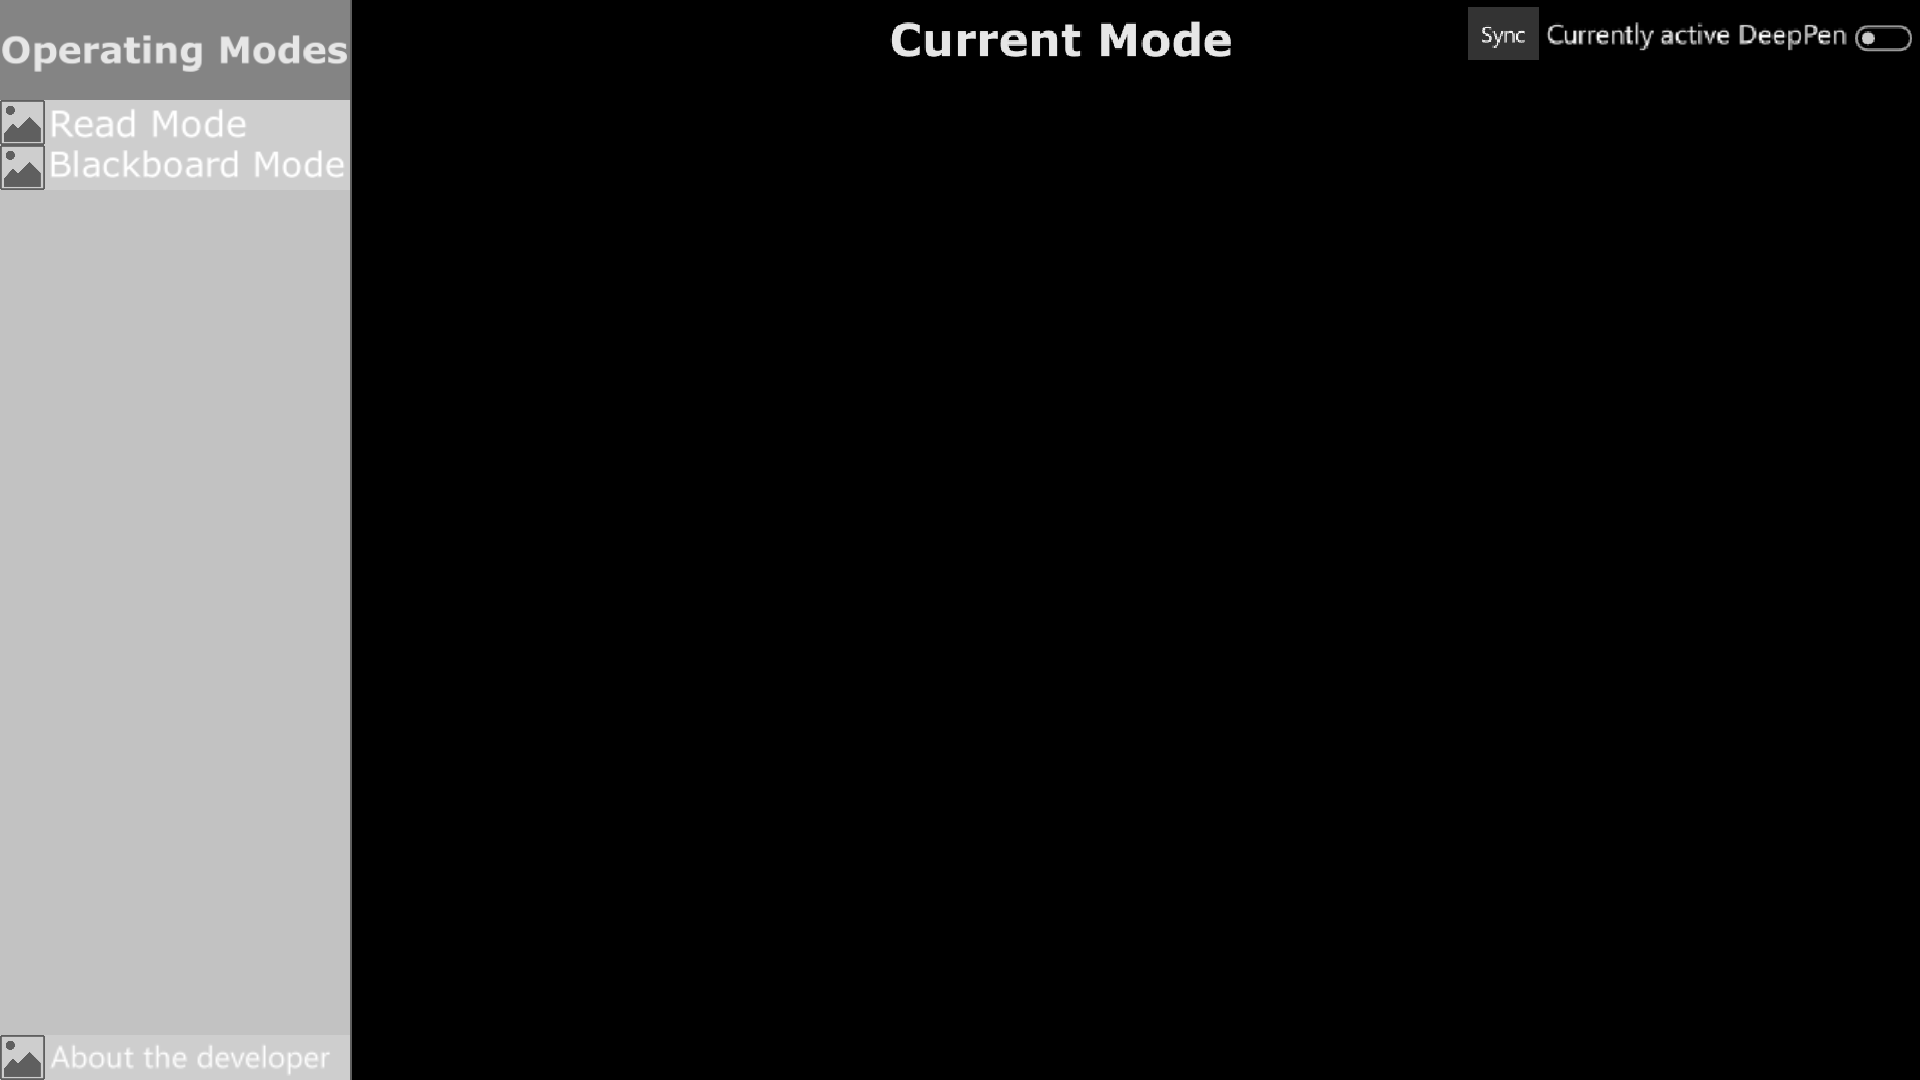
\includegraphics[angle=270,width=0.49\textwidth]{capturas/DisenoUsuario2.png}\\[-0,35cm]
    \caption{Boceto en QT Design Studio}
\end{figure}

\begin{figure}[h]
    \centering
    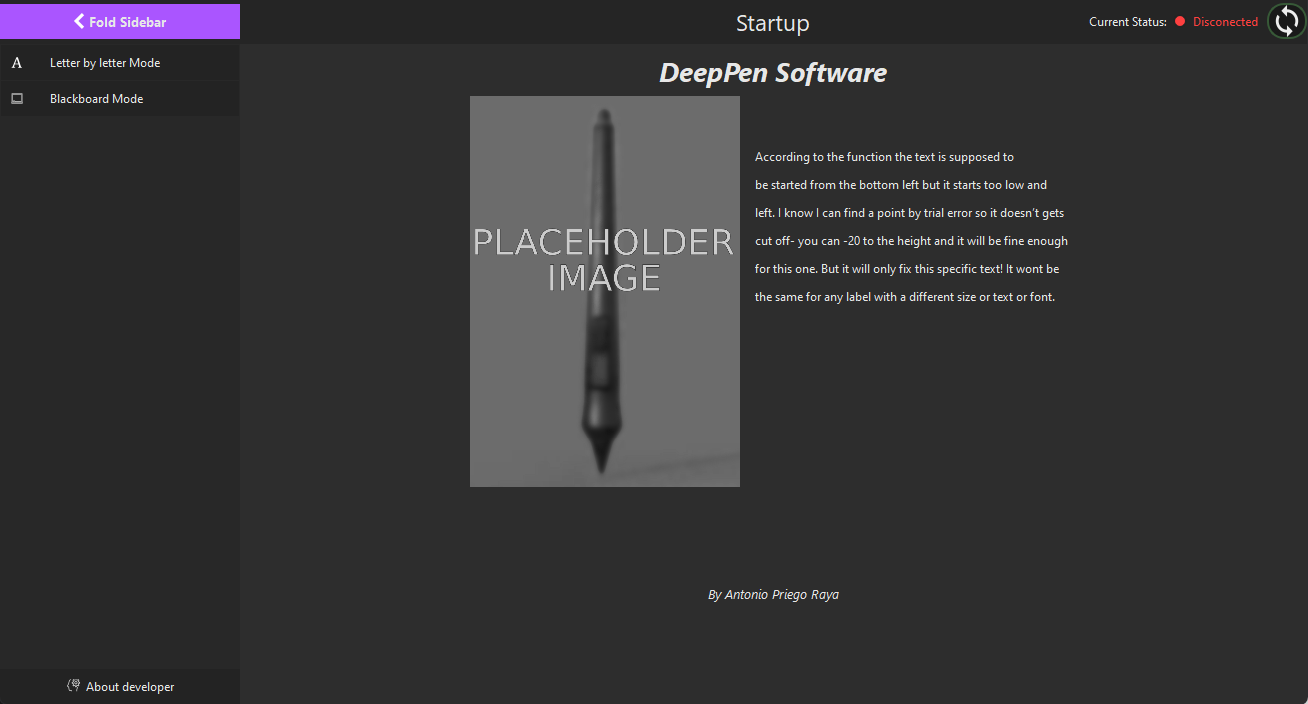
\includegraphics[angle=90,width=1\textwidth]{capturas/Interfaz.png}\\[-0,35cm]
    \caption{Resultado de la implementación de la interfaz de usuario}
\end{figure}

\chapter{Encapsulado}
\section{Modelos 3D\label{modelos}}
\begin{figure}[h]
    \centering
    \subfloat[\href{https://github.com/AntonioPriego/SmartPen/tree/main/SmartPenModel/Components/cilindroAlto}{cilindroAlto}]{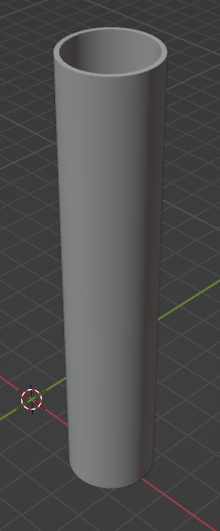
\includegraphics[width=0.185\textwidth]{capturas/cilindroAlto.png}}
    \hfill
    \subfloat[\href{https://github.com/AntonioPriego/SmartPen/tree/main/SmartPenModel/Components/slotBateria}{slotBateria}]{\includegraphics[width=0.405\textwidth]{capturas/slotBatería.png}}
    \hfill
    \subfloat[\href{https://github.com/AntonioPriego/SmartPen/tree/main/SmartPenModel/Components/cilindroBajo}{cilindroBajo}]{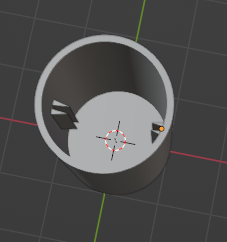
\includegraphics[width=0.4\textwidth]{capturas/cilindroBajo.png}}
    \caption{Componentes útiles del encapsulado}
\end{figure}

  \begin{figure}[h]
    \centering
    \subfloat[\href{https://github.com/AntonioPriego/SmartPen/tree/main/SmartPenModel/Components/clip}{clip}]{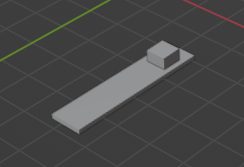
\includegraphics[width=0.27\textwidth]{capturas/clip.png}}
    \hfill
    \subfloat[\href{https://github.com/AntonioPriego/SmartPen/tree/main/SmartPenModel/Components/punta}{punta}]{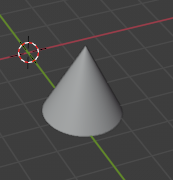
\includegraphics[width=0.18\textwidth]{capturas/punta.png}}
    \hfill
    \subfloat[\href{https://github.com/AntonioPriego/SmartPen/tree/main/SmartPenModel/Components/semiEsfera}{semiEsfera}]{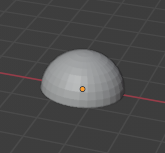
\includegraphics[width=0.21\textwidth]{capturas/semiEsfera.png}}
    \caption{Decoración del encapsulado}
  \end{figure}

\section{Resultado de integrar todo en el encapsulado\label{encapsulado}}
\begin{figure}[h]
    \centering
    \subfloat[SmartPen vista frontal]{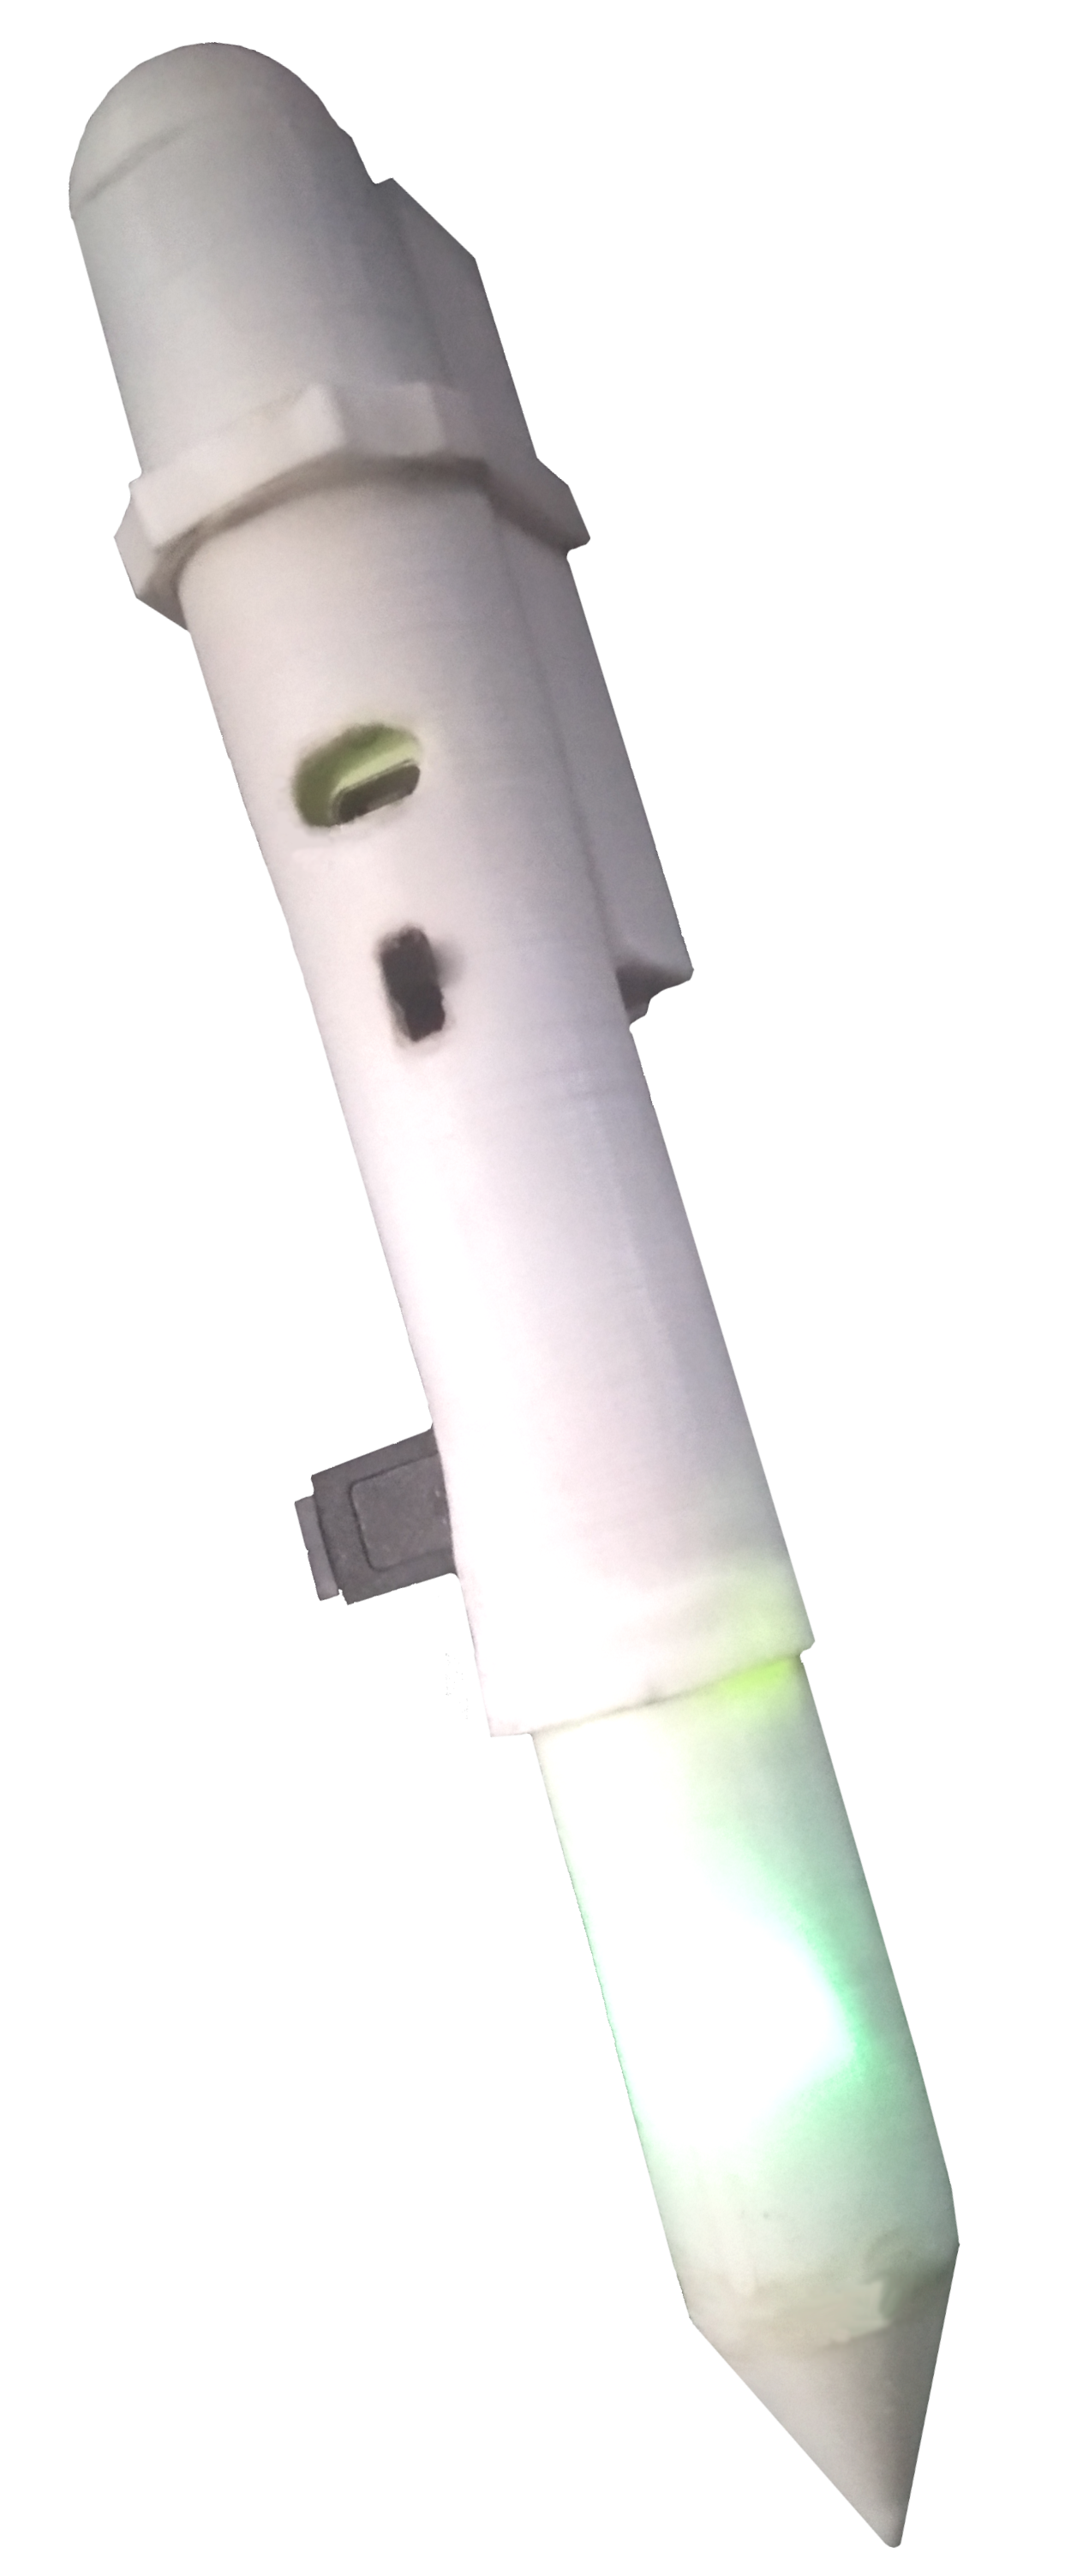
\includegraphics[width=0.48\textwidth]{capturas/SmartPen.png}}
    \hfill
    \subfloat[SmartPen vista trasera]{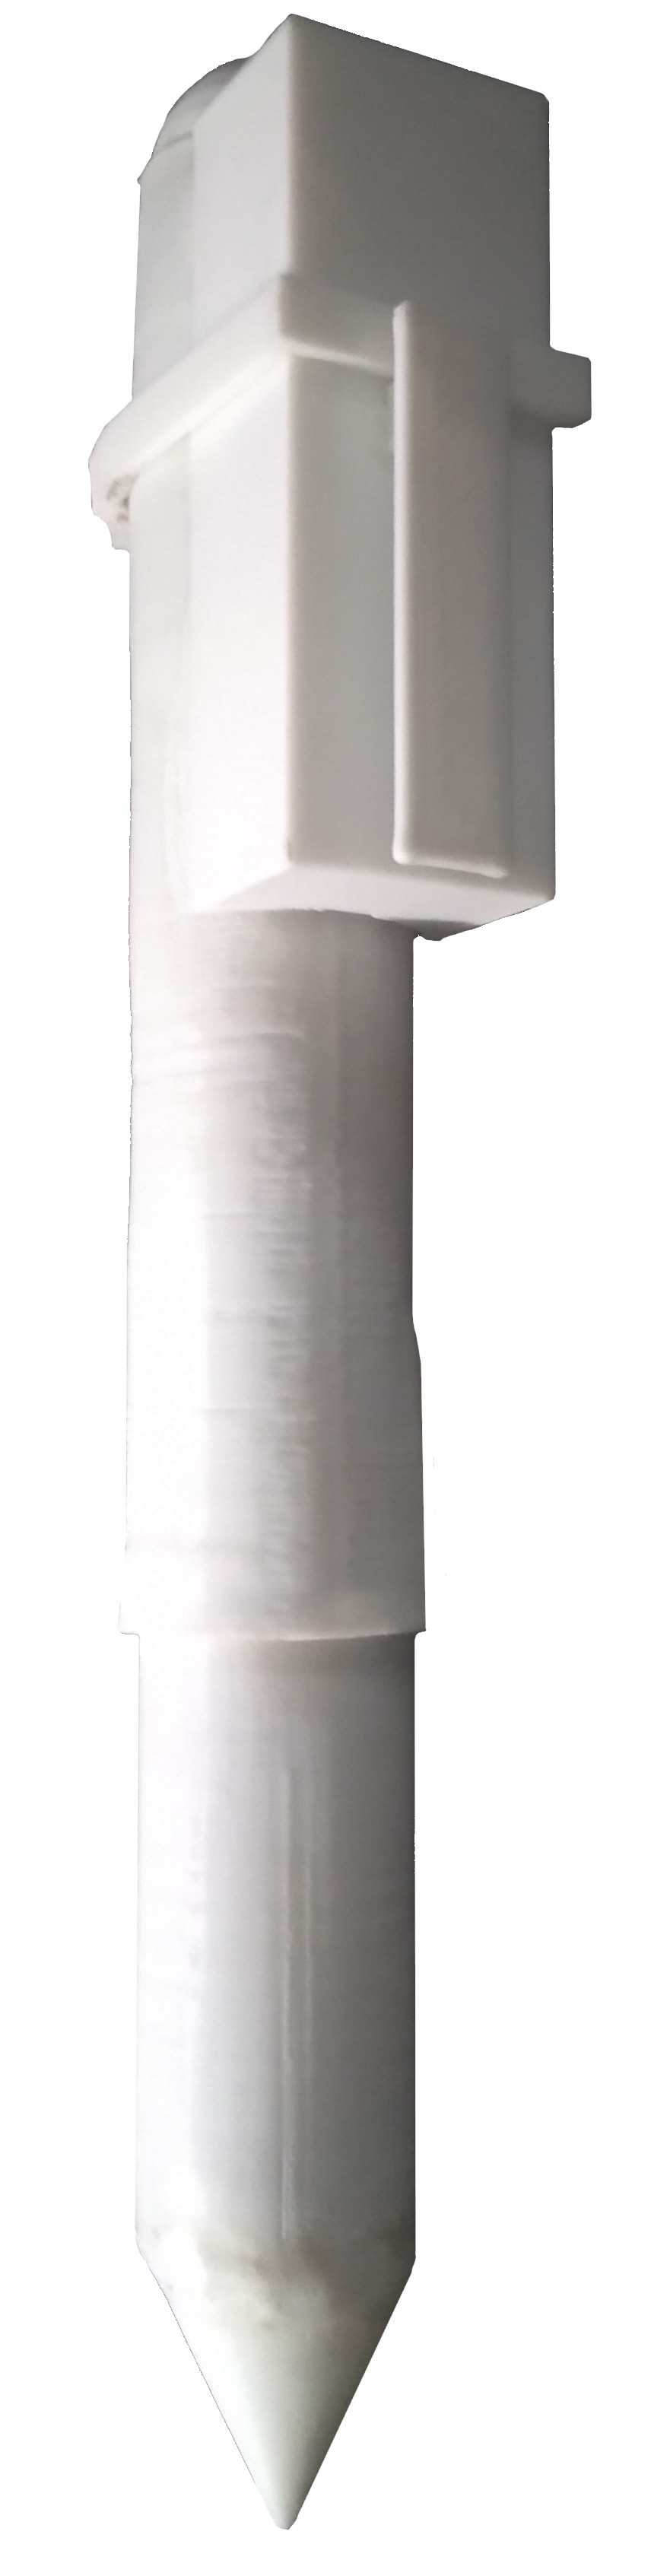
\includegraphics[width=0.29\textwidth]{capturas/SmartPenTrasero.png}}
    \caption{SmartPen}
  \end{figure}

\end{appendices}

	\pagebreak
	\begin{figure}
		\centering
		
\includegraphics[width=0.25\textwidth]{imagenes/GitHubIcon.png}
	\end{figure}
	\Huge \centering Github del proyecto\\ \Large \url{https://github.com/AntonioPriego/SmartPen}\\
	\begin{figure}[h]
		\centering
		
\includegraphics[width=0.25\textwidth]{imagenes/QRGitHub.png}
	\end{figure}
	\cleardoublepage
\end{document}

